\subsection{Data Science and Machine Learning}
\label{sec:DSML}
\begin{tcolorbox}[title=From Data to Wisdom]
Data is not information, information is not knowledge, knowledge is not understanding, understanding is not wisdom. \\[-0.6cm]
\begin{flushright}
-- attributed to Cliff Stoll, \textit{Nothing to Hide: Privacy in the 21st Century}, 2006
\end{flushright}
\end{tcolorbox}
\noindent In October 2012, the \textit{Harvard Business Review} published an article calling data science the ``sexiest job of the 21st century'', and comparing data scientists with the ubiquitous Wall Street ``quants'' of the '80s and '90s: a data scientist is a ''hybrid of data hacker, analyst, communicator, and trusted adviser'' \cite{DSML_HBR} -- data science is hot and everybody wants in! \par Would-be data scientists are usually introduced to the field \text{via} machine learning algorithms and applications. Much could be said about those; the material presented here is not meant to constitute a complete survey of the field (multiple references are provided for the interested reader).  \newl  
In particular, we will take a brief look at: 
\begin{itemize}[noitemsep]
    \item the \textbf{fundamentals} of data science;
    \item \textbf{association rules} mining;
    \item \textbf{supervised learning and classification}, with a focus on \textbf{decision trees};
    \item \textbf{unsupervised learning and clustering}, with a focus on \textbf{$k-$means};
    \item some of the common \textbf{issues and challenges} linked to the data science process;
    \item an introduction to \textbf{artificial} (or augmented) \textbf{intelligence and deep learning}, \textit{via} simple neural networks;
    \item \textbf{text mining and natural language processing}, with a focus on \textbf{sentiment analysis};
    \item the basic principles of \textbf{distributed computing} for Big Data analysis, and 
    \item a few other topics. 
\end{itemize}
\subsubsection{Fundamentals}
\begin{tcolorbox}[title=From Data to Wisdom]
We learn from failure, not from success! \\[-0.6cm]
\begin{flushright}
-- Bram Stoker, \textit{Dracula}
\end{flushright}
\end{tcolorbox}
\noindent Hilary Mason, a noted data scientist, has described data science as 
\begin{quote}
    the \textbf{working intersection} of statistics, engineering, computer science, domain expertise, and ``hacking.'' 
\end{quote}
In her view (which we share), it involves two main thrusts: \textbf{analytics} (which is to say, counting things) and \textbf{inventing new techniques} to draw insights from data \cite{DSML_M}.
\newl A more pragmatic approach is to define data science as ``the collection of processes by which we extract useful and \textbf{actionable insights} from data'' (paraphrased from Ted Kartler).
\paragraph{Types of Learning} 
As humans, we learn (at all stages) by first taking a look around, and then by answering questions, testing hypotheses, creating concepts, making predictions, creating categories and classifying objects, and grouping objects. In a way, the idea behind data science is to try to teach our machines (and thus, ultimately, ourselves) to gleam insight from data, and how to do this properly and efficiently, free of biases and pre-conceived notions -- in other words, \begin{quote} \textbf{can we design algorithms that can learn?}\end{quote} The simplest data science method, thus, is to \textbf{explore the data} (or at a representative sample), providing a summary through basic statistics -- mean, mode, histograms, etc.; making its multi-dimensional structure evident through data data visualisation; and looking for consistency, considering what is in there and what is missing.
\begin{center}
    \rule{0.5\textwidth}{.4pt}
\end{center}  In the data science context, we identify two substantially more sophisticated types of leaning:  \textbf{supervised} and  \textbf{unsupervised}. \textbf{Supervised learning} is akin to ``learning with a teacher.'' Typical tasks include \textit{classification}, \textit{regression}, \textit{rankings}, and \textit{recommendations}. In supervised learning, algorithms use \textbf{labeled training data} to build (or train) a predictive model (i.e. ``students give an answer to each exam question based on what they learned from worked-out examples provided by the teacher/textbook''); each algorithm's performance is evaluated using \textbf{test data} for which the label is known but not used in the prediction  (i.e. ``the teacher provides the correct answers and marks the students' exam questions using the key''.)\par
\textbf{Unsupervised learning} is akin to ``self-learning by grouping similar exercises together as a study guide.'' Typical tasks include \textit{clustering}, \textit{association rules discovery}, \textit{link profiling}, and \textit{anomaly detection}. Unsupervised algorithms use \textbf{unlabeled data} to find natural patterns in the data  (i.e. ``the teacher is not involved in the discovery process''); the drawback is that accuracy \textbf{cannot be evaluated} with the same degree of satisfaction (i.e. ``students might end up with different groupings'').\par In the same vein, data scientists also recognise \textbf{semi-supervised learning} when some data points have labels but most do not, which is often the case when acquiring data is costly (``the teacher provides worked-out examples and a list of unsolved problems to try out; the students try to find similar groups of unsolved problems and compare them with the solved problems to find close matches'') and \textbf{reinforcement learning}, where an agent attempts to collect as much (short-term) reward as possible while minimising (long-term) regret (``embarking on a Ph.D. with an advisor... with highs and lows and \textit{perhaps} a solution at the end of the day?''). Some data science techniques fit into both camps; others can be either supervised or unsupervised, depending on how they are applied.
\begin{center}
    \rule{0.5\textwidth}{.4pt}
\end{center} 
In supervised learning, there are fixed \textbf{targets} against which to train the model (such as age categories, or plant species) -- the categories (and their number) are known prior to the analysis.  In unsupervised learning, we don't know what the target is, or even if there is one -- we are simply looking for \textbf{natural groups} in the data (such as junior students who like literature, have longish hair, and know how to cook \textit{vs.} students who are on a sports team and have siblings \textit{vs.} financial professionals with a penchant for superhero movies, craft beer and Hello Kitty \textit{vs.} ... ). The distinction is \textbf{crucial}. Take some time to make sure you master it. \label{unsl}
\paragraph{Data Science Tasks}
As we have mentioned previously, quantitative methods are only really interesting to clients when they help them ask and answer useful questions. Compare, for instance:
\begin{itemize}[noitemsep] 
\item\textbf{Analytics} -- ``How many clicks did this link get?''
\item \textbf{Data Science} --  ``Based on the previous history of clicks on links of this publisher's site, can I predict how many people from Manitoba will read this specific page in the next three hours?'' or ``Is there a relationship between the history of clicks on links and the number of people from Manitoba who will read this specific page?''
\item \textbf{Quantitative Methods} -- ``We have no similar pages whose history could be consulted to make a prediction, but we have reasons to believe that the number of hits will be strongly correlated with the temperature in Winnipeg. Using the weather forecast over the next week, can we predict how many people will access the specific page during that period? ''
\end{itemize}
Data science models are usually \textbf{predictive} (not \textbf{explanatory}): they show connections, and exploit correlations to make predictions, but they don't reveal why such connections exist. Quantitative methods, on the other hand, usually assume a certain level of causal understanding based on various \textbf{first principles}. That distinction is not always understood properly by clients and consultants alike. 
\begin{center}
    \rule{0.5\textwidth}{.4pt}
\end{center}
\textbf{IMPORTANT NOTE:} this is as good a time as any to remind you that not every situation calls for data science (or even analytics). The recent drive towards data science has a ``snake oil'' feel to it, in our opinion (and in the opinion of a number of qualified commentators \cite{DSML_F}); vendors and pundits have conducted a near-perfect marketing campaign for so-called ``Big Data'' and Data Science in general, but ask 10 stakeholders what these concepts mean and you're likely to get 10 different answers. \par As a result, clients will often expect you to solve their problem using the latest data science gizmos even if they have no bearing on the problem at hand. Understanding the \textbf{limitations} of the methods and focusing on the client's explicit and tacit \textbf{needs} might help you avoid that particular quagmire.  
\begin{center}
    \rule{0.5\textwidth}{.4pt}
\end{center}
Common data science tasks (with representative questions) include \cite{DSML_PF}:
\begin{itemize}[noitemsep]
\item \textbf{classification} and \textbf{class probability estimation} -- 
which undergraduates are likely to succeed at the graduate level?
\item \textbf{value estimation} -- how much is a given client going to spend at a restaurant?
\item \textbf{similarity matching} -- which prospective clients are most similar to a company's establishes best clients?
\item \textbf{clustering} -- do signals from a sensor form natural groups?
\item \textbf{association rules discovery} -- what books are commonly purchased together at an online retailer?
\item \textbf{profiling} and \textbf{behaviour description} -- what is the typical cell phone usage of this customer's segment?
\item \textbf{link prediction} -- J. and K. have 20 friends in common: perhaps they'd be great friends?
\end{itemize}
A classic example is provided by the UCI Machine Learning Repository  Mushroom Dataset \cite{DSML_UCI}. Consider \textit{Amanita muscaria}, a specimen of which is shown in Figure~\ref{fig:DSML_am}.
\begin{figure}[!t]
\centering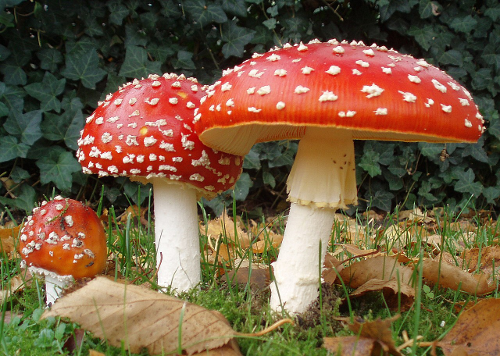
\includegraphics[width=200pt]{images/DSML/Amanita_muscaria.png}\caption[\small \textit{Amanita muscaria}]{\small \textit{Amanita muscaria} (or fly agaric), in the wild. Does it look dangerous to you?}\label{fig:DSML_am}\hrule
\end{figure}\afterpage{\FloatBarrier}
Is it \textbf{\textcolor{Green}{edible}}, or \textbf{\textcolor{Red}{poisonous}}? 
\newl There is a simple way to get an answer -- eat it, wait, and see. If you do not die or get sick upon ingestion, it was \textbf{\textcolor{Green}{edible}}; otherwise it was \textbf{\textcolor{Red}{poisonous}}.\par This test in unappealing for various reasons, however. apart from the obvious risk of death, we might not learn much from the experiment; it is possible that this specific specimen was poisonous due to some mutation or some other factor, and that fly agaric is actually edible in general, or \textit{vice-versa}.\newl A predictive model, which would use features of a vast collection of mushroom species and specimens (including whether they were poisonous or edible) could help us some shed light on the matter: what do poisonous mushrooms have in common? what properties do edible mushrooms share?  (note that this is not the same as understanding \textit{why} a mushroom is poisonous or edible).\newl For instance, let's say that \textit{Amanita muscaria} has the following features: 
\begin{quote}
    \textbf{habitat}: woods; \textbf{gill size}: narrow; \textbf{spores}: white; \textbf{odor}: none.
\end{quote}
We do not know, \textit{a priori}, whether it is \textbf{\textcolor{Red}{poisonous}} or \textbf{\textcolor{Green}{edible}}. Is the available information sufficient to answer the question? On its own, it is not (a mycologist could perhaps deduce the answer from these features alone, but she would be using her experience with fungi to make a prediction, and so would not be looking at features in a vacuum). But we can use past data, with correct \textbf{\textcolor{Green}{edible}} or \textbf{\textcolor{Red}{poisonous}} labels, to build  various supervised \textbf{classification} models to attempt to answer the question. Such a model, a \textbf{decision tree}, is shown in Figure~\ref{fig:DT_mushroom1}.  The model prediction for \textit{Amanita muscaria} follows the \textbf{decision path} shown in Figure~\ref{fig:DT_mushroom2}: 
\begin{enumerate}[noitemsep]
    \item some mushroom \textbf{odors} (musty, spicy, etc.) are associated with poisonous mushrooms, some (almond, anise) with edible mushrooms, but there are  mushrooms with no specific odor in either category -- that feature does not provide enough information to classify \textit{Amanita muscaria} and we need to incorporate additional features into the decision path;
    \item among mushrooms with no specific odor, some \textbf{spore colours} (black, brown, etc.) are associated with edible mushrooms, some (almond, anise) with poisonous mushrooms, but there are  mushrooms with white spores in either category -- the combination `no odor and white spores' does not provide enough information to classify \textit{Amanita muscaria} and we need to incorporate additional features into the decision path;
    \item among mushrooms of no specific odor with white spores, some \textbf{habitats} (grasses, paths, wastes) are associated with edible mushrooms, but there are  mushrooms in either category that are found in the woods -- the combination `no odor, white spores, found in the woods' does not provide enough information to classify \textit{Amanita muscaria} and we need to incorporate additional features into the decision path;
    \item among forest mushrooms of no specific odor with white spores, a broad \textbf{gill size} is associated with edible mushrooms, whereas a narrow gill size is associated with poisonous mushrooms. As \textit{Amanita muscaria} is a a narrow-gilled forest mushroom of no specific odor with white spores, the decision path predicts that it is \textbf{\textcolor{Red}{poisonous}}. 
\end{enumerate}   
\begin{figure}[!t]
\begin{subfigure}[b]{0.57\textwidth}
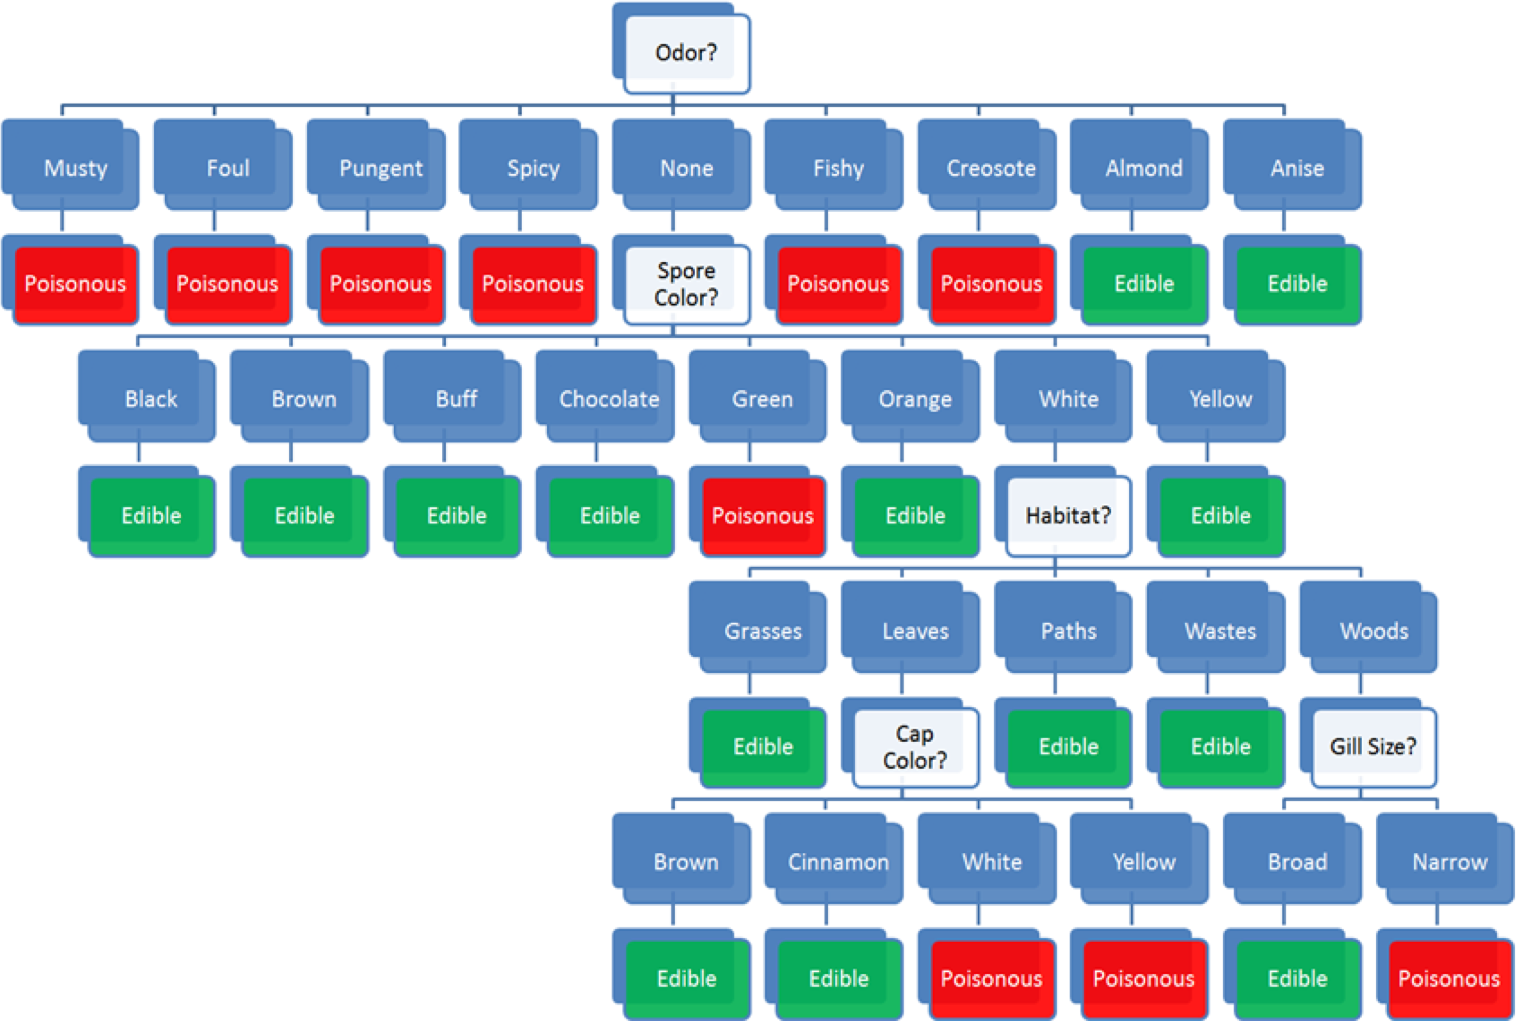
\includegraphics[height=0.3\textheight]{images/DSML/mushroom1.png}\caption{\small Decision tree} \label{fig:DT_mushroom1}
\end{subfigure}\qquad
\begin{subfigure}[b]{0.3\textwidth}
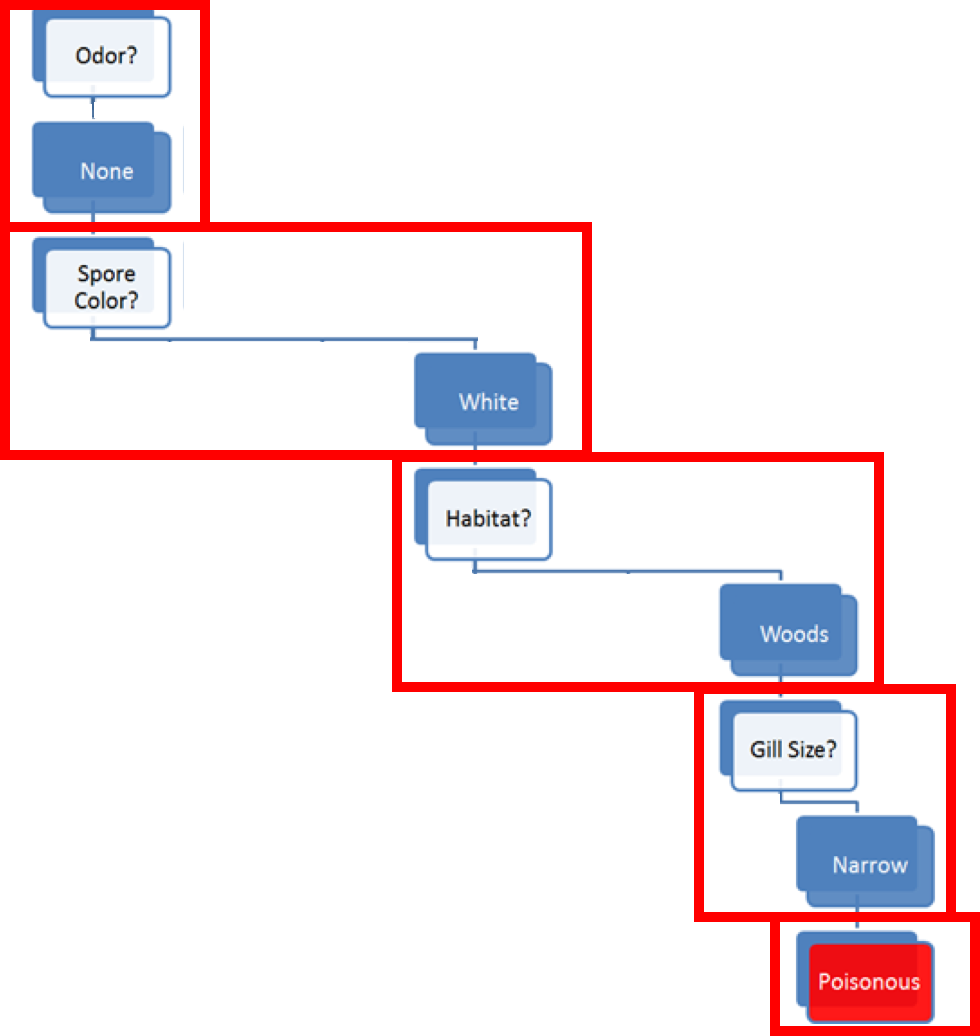
\includegraphics[height=0.3\textheight]{images/DSML/mushroom2.png}\caption{\small Decision path} \label{fig:DT_mushroom2}
\end{subfigure}
\caption[\small Decision tree for the mushroom classification problem]{\small Decision tree for the mushroom classification problem, with decision path for \textit{Amanita muscaria}.}\label{fig:DT_mushroom}\hrule
\end{figure}\afterpage{\FloatBarrier}
The model \textbf{does not explain why} this particular combinations of features is associated with poisonous mushrooms -- the decision path is not \textbf{causal}. Would you or a client have trusted an \textbf{\textcolor{Green}{edible}} prediction? What's the true cost of making a classification mistake? Is the data on which the model is built representative? What do we need to know about the model in order to trust it? 


\subsubsection{Association Rules}
\begin{tcolorbox}[title=Tufte's Rejoinder]
Correlation isn't causation. But it's a big hint. \\[-0.6cm]
\begin{flushright}
-- E. Tufte
\end{flushright}
\end{tcolorbox}
\noindent Association rules discovery is a type of unsupervised learning that finds \textbf{connections} among the attributes and levels (and combinations of attribute and levels) of a dataset's observations.
\newl For instance, we might analyse a dataset on the physical activities and purchasing habits of North Americans and discover that 
\begin{itemize}[noitemsep]
\item \textit{runners who are also triathletes} (the \textbf{premise}) tend to \textit{drive Subarus, drink microbrews, and use smart phones} (the \textbf{conclusion}), or 
\item individuals who have purchased home gym equipment are unlikely to be using it 1 year later, say. 
\end{itemize}
As Tufte reminds us on the previous page, correlation is not causation. Being a triathlete does not cause one to drive a Subaru, but a connection exists -- enough so that in 2018, some Subaru dealerships in Qu\'ebec were offering to pay the registration fee at an IRONMAN 70.3 competition with the purchase of a new vehicle! 
\begin{center}
    \rule{0.5\textwidth}{.4pt}
\end{center}
Association rules discovery is also known as \textbf{market basket analysis} after its original application, in which supermarkets record the contents of shopping carts (the baskets) at check-outs to determine which items are frequently purchased together. Bread and milk might often be purchased together, for instance, but that is unlikely to be interesting given the frequency of market baskets containing milk or bread (in the mathematical sense of "or"). Wieners and mustard, on the other hand, might be purchased together more often than one would expect given how frequently both items are purchased; perhaps they are likely to be purchased as a pair, but not so likely to be purchased individually. 
\newl It is not too difficult to see how this information could potentially be used to help supermarkets turn a profit. Announcing or advertising a sale on hot dogs while simultaneously (and quietly) raising the price of condiments could have the effect of bringing in a higher number of customers into the store, increasing the sale volume for both items while keeping the combined price of the two items constant (banking on the fact that customers are unlikely to shop around to get the best deal on hot dogs AND condiments). 
\newl A (possibly) apocryphal story shows the limitations of association rules: a supermarket found an association rule linking the purchase of beer and diapers and consequently moved its beer display closer to its diapers display, having confused correlation and causation. Purchasing diapers does not cause one to purchase beer (or \textit{vice-versa}); it could simply be that parents of newborns have little time to visit public houses and bars, and whatever drinking they do will be done at home. Rumour has it that the experiment was neither popular nor successful.    
\begin{center}
    \rule{0.5\textwidth}{.4pt}
\end{center}
Other applications and uses exist, such as 
\begin{itemize}[noitemsep]
\item finding \textbf{related concepts} in text documents -- looking for pairs (triplets, etc) of words that represent a joint concept: 
{San Jose, Sharks}, {Michelle, Obama}, etc.;
\item detecting \textbf{plagiarism} -- looking for specific sentences that appear in multiple documents, or for documents that share specific sentences; 
\item identifying \textbf{biomarkers} -- searching for diseases that are frequently associated with a set of biomarkers;
\item making predictions and decisions based on association rules (care must be taken to avoid a number of pitfalls);
\item altering circumstances or environment to take advantage of these correlations (when a causal effect is suspected);
\item using connections to modify the likelihood of certain outcomes; 
\item imputing missing data, and 
\item text autofill and autocorrect.
\end{itemize}
Other uses and examples can be found in \cite{DSML_ES, DSML_BSHWJM, DSML_GRVC}.
\paragraph{Causation and Correlation}
Association rules can automate \textbf{hypothesis discovery}, but one must remain correlation-savvy (which is less prevalent among quantitative specialists than one might hope, in our experience). If attributes $A$ and $B$ are shown to be correlated in a dataset, there are four possibilities:
\begin{itemize}[noitemsep]
    \item $A$ and $B$ are correlated entirely by chance in this particular dataset;
    \item $A$ is a relabeling of $B$ (or \textit{vice-versa});
    \item $A$ causes $B$ (or \textit{vice-versa}), or 
    \item some combination of other attributes $C_1,\ldots,C_n$ (which may not be available in the dataset) cause both $A$ and $B$.
\end{itemize}
E. Siegel provides a number of examples of the confusion in \cite{DSML_ES}: \begin{itemize}[noitemsep]
\item Walmart has found that the sales of strawberry Pop-Tarts increase about seven-fold in the days preceding the arrival of a hurricane;
\item Xerox hourly employees engaged in front-line service and sales-based positions who use Chrome and Firefox browsers perform better on employment assessment metrics and stay on longer, or
\item University of Cambridge researchers fround that liking ``Curly Fries'' on Facebook is predictive of high intelligence.
\end{itemize}
It can be tempting to try to \textbf{explain} these results (again from \cite{DSML_ES}): perhaps 
\begin{itemize}[noitemsep]
\item in preparation before an act of nature, people stock up on comfort or nonperishable foods;
\item the fact that an employee takes the time to install another browser shows that they are an informed consumer and that they care about their productivity, or
\item an intelligent person liked this Facebook page first, and her friends saw it, and liked it too, and since intelligent people have intelligent friends (?) it spread to them and so on.
\end{itemize}
These explanations \textit{might} very well be the right ones, but there is nothing in the data to support them. Association rules discovery \textbf{finds} interesting rules, but it does not explain them. 
\begin{center}
    \rule{0.5\textwidth}{.4pt}
\end{center}
\textbf{IMPORTANT NOTE:} you might not have much control over the matter as a consultant, but do whatever is in your power to avoid the accompanying headlines (or briefing to ministers) to be along the lines of 
\begin{itemize}[noitemsep]
\item ``Pop-Tarts'' help hurricane victims get back on their feet; 
\item Using Chrome of Firefox improves employee performance, or 
\item Eating curly fries makes you more intelligent. 
\end{itemize}
\paragraph{Definitions} A rule $X\to Y$ is a statement of the form ``if $X$ (the \textbf{premise}) then $Y$ (the conclusion)'' built from any logical combinations of a dataset attributes. In practice, a rule \textbf{does not need to be true for all observations} in the dataset -- there could be instances where the premise is satisfied but the conclusion is not. In fact, it is often the case that the ``best'' rules are those which are only accurate 10\% of the time, as opposed to rules which are only accurate is only 5\% of the time, say. As always, \textbf{it depends on the context}.\newl 
To determine a rule's strength, we compute various rule metrics, such as the:
\begin{itemize}[noitemsep]
\item \textbf{support} (coverage) which measures the frequency at which a rule occurs in a dataset -- low coverage values indicate rules that rarely occur;
\item \textbf{confidence} (accuracy) which measures the reliability of the rule: how often does the conclusion occur in the data given that the premises have occurred --  rules with high confidence are ``truer'', in some sense;
\item \textbf{interest} which  measures the difference between its confidence and the relative frequency of its conclusion -- rules with high absolute interest are ... well, more interesting than rules with small absolute interest, and  
\item \textbf{lift}, which measures the increase in the frequency of the conclusion which can be explained by the premises -- in a rule with a high lift ($>1$), the conclusion occurs more frequently than it would if it was independent of the premises.
\end{itemize}
If $N$ is the number of observations in the dataset and $\textrm{Freq}(A)\in [0,N]$ represents the count of the dataset's observations for which property $A$ holds, then we can compute the metrics as follows: 
\begin{align*}
    \textrm{Support}(X\to Y)&=\frac{\textrm{Freq}(X\cap Y)}{N}\in[0,1] \\ 
    \textrm{Confidence}(X\to Y)&=\frac{\textrm{Freq}(X\cap Y)}{\textrm{Freq}(X)}\in[0,1] \\ 
    \textrm{Interest}(X\to Y)&=\textrm{Confidence}(X\to Y) - \frac{\textrm{Freq}(Y)}{N} \in [-1,1] \\ 
\textrm{Lift}(X\to Y) &=\frac{N^2\cdot \textrm{Support}(X\to Y)}{\textrm{Freq}(X)\cdot \textrm{Freq}(Y)} \in (0,N^2)
\end{align*}
The support is the proportion of instances where the premise and the conclusion occur together; the confidence is the proportion of instances where the conclusion occurs when the premise occurs, and so forth.
\begin{center}
    \rule{0.5\textwidth}{.4pt}
\end{center}
A simple example will serve to illustrate these concepts. Consider a (hypothetical) music dataset containing data for $N=15,356$ Chinese music lovers and a \textbf{candidate rule} RM: \begin{quote}``If an individual is born before 1986 ($X$), then they own a copy of Teresa Teng's \textit{The Moon Represents My Heart}, in some format ($Y$)''. 
\end{quote}
Let's assume further that   
\begin{itemize}[noitemsep]
    \item $\textrm{Freq}(X)=3888$ individuals were born before 1986;
\item $\textrm{Freq}(Y)=9092$ individuals own a copy of \textit{The Moon Represents My Heart}, and 
\item $\textrm{Freq}(X\cap Y)=2720$ individuals were born before 1986 and own a copy of \textit{The Moon Represents My Heart}.
\end{itemize}
We can easily compute the 4 metrics for RM: 
\begin{align*}
    \textrm{Support}(\textrm{RM})&=\frac{2720}{15,536}\approx 18\% \\ 
    \textrm{Confidence}(\textrm{RM})&=\frac{2720}{3888}\approx 70\% \\ 
    \textrm{Interest}(\textrm{RM})&=\frac{2720}{3888}-\frac{9092}{15,356}\approx 0.11 \\ 
\textrm{Lift}(\textrm{RM}) &=\frac{15,356^2\cdot 0.18}{3888\cdot 9092} \approx 1.2.
\end{align*}
These values are easy to interpret: RM occurs in 18\% of the instances and it is true in 70\% of the instances where the individual was born prior to 1986. This would seem to make RM a meaningful rule about the dataset -- being older and owning that song are linked properties! But if being younger and not owning that song are not also linked, the statement is weaker than it appears at a first glance. As it happens, RM's lift is 1.2, which can be rewritten as $1.2\approx \frac{0.70}{0.56}$, which means that 56\% of younger individuals also own the song. The ownership rates between the two age categories are different, but perhaps not as significantly as one would deduce using the confidence and support alone, which is reflected by the low interest (0.11). \begin{center}
    \rule{0.5\textwidth}{.4pt}
\end{center} \textbf{IMPORTANT NOTE:} There will be times when an interest of 0.11 in a rule will be considered a smashing success, when a lift of 15 will not be considered that significant, and so forth. It's difficult to give hard and fast rules about absolute thresholds: it always depends on the context, and on comparing metric values with the dataset's other rules. In general, there is value in conducting preliminary exploration of the space of association rules (using domain expertise when appropriate) to determine reasonable threshold ranges for the specific situation; candidate rules are discarded or retained depending on these metric thresholds. 
\paragraph{Rule Generation} When we are given a rule (or rules), it is straightforward to evaluate it using various metrics. The real  challenge of association rules discovery is in \textbf{generating} a set of candidate rules which are likely to be retained, without wasting time generating rules which are likely to be discarded. That is easier said than done.  \par 
An \textbf{item set} (or instance set) is a list of attributes and values. A set of rules can be created by adding `IF ... THEN' blocks to the instances. From the instance set 
\begin{quote}$\{ \textrm{membership} = \textrm{True}, \textrm{age} = \textrm{Youth}, \textrm{purchasing} = \textrm{Typical} \}$ \end{quote}
we can create the rules
\begin{itemize}[noitemsep]
    \item IF $(\textrm{membership} = \textrm{True}$ AND $\textrm{age} = \textrm{Youth}$) THEN $\textrm{purchasing} = \textrm{Typical}$;
    \item IF $\textrm{membership} = \textrm{True}$ THEN ($\textrm{age} = \textrm{Youth}$ AND $\textrm{purchasing} = \textrm{Typical}$);
    \item IF $\varnothing$ THEN ($\textrm{membership} = \textrm{True}$ AND $\textrm{age} = \textrm{Youth}$ AND $\textrm{purchasing} = \textrm{Typical}$); etc.
\end{itemize}
Now, consider an item set $\mathcal{C}$ with $n$ members (that is to say, $n$ attribute/level pairs). In a rule derived from $\mathcal{C}$, each of the $n$ members shows up either in the premise or in the conclusion; there are thus $2^n$ such rules. The rule where each member is part of the premise (that is, the rule without a conclusion) is nonsensical and is not allowed, and so $2^n-1$ rules can be derived from $\mathcal{C}$. The \textbf{number of rules increases exponentially} when the \textbf{number of features increases linearly}. This combinatorial explosion is a problem -- it instantly disqualifies the \textbf{brute force} approach (simply listing all possible item sets in the data and generating all rules from those item sets) for any dataset with a realistic number of attributes. How do we generate \textbf{promising} candidate rules, in general?
\newl The \textbf{apriori} algorithm is an early attempt to bypass that difficulty. It was developed initially for transaction data (but every reasonable dataset can be transformed into a transaction dataset using dummy variables). This algorithm attempts to find \textbf{frequent item sets} from which to build candidate rules, instead of building rules from \textit{all} possible item sets.
\par It starts by identifying frequent \textbf{individual items} in the database and extends those that are retained into larger and larger item sets, assuming that these new sets are still found \textbf{frequently enough} in the data. In the technical jargon, we say that \textit{apriori} uses a \textbf{bottom-up approach} and the \textbf{downward closure property of support}. \par The savings come from the fact that the algorithm prunes candidates with \textbf{infrequent sub-patterns} and removes them from consideration for any future item set: if a 1-item set is not considered to be frequent enough, any 2-item set containing it is also infrequent (see Table~\ref{tab:NHL} for an illustration). \par Of course, this requires a support threshold \textbf{input} (and there is no clear way to select that threshold, although it has to be set sufficiently high to minimise the number of frequent item sets that are being considered). The algorithm terminates when no further successful extensions are found.
\begin{itemize}[noitemsep] \item \textbf{Strengths:} easy to implement, easily parallelized \cite{DSML_MMD}.
\item \textbf{Limitations:} slow, requires frequent data set scans, not ideal for finding rules for infrequent and rare item sets. 
\end{itemize}
Other, more efficient, algorithms have since displaced it (although it does have historical value):
\begin{itemize}[noitemsep]
\item \textbf{Max-Miner} tries to identify frequent item sets without enumerating them -- it performs jumps in space instead of using bottom-up approach; 
\item \textbf{Eclat} is faster and uses depth-first search, but requires extensive memory storage (apriori and eclat are both implemented in the \texttt{R} package \texttt{arules}).
\end{itemize}
\paragraph{Notes}
How \textbf{reliable} are association rules? What is the likelihood that they occur entirely \textbf{by chance}? How \textbf{relevant} are they? Can they be generalised \textbf{outside} the dataset, or to \textbf{new} data streaming in?  These questions are notoriously difficult to solve for association rules discovery, but \textbf{statistically sound association discovery} can help reduce the risk of finding spurious associations to a user-specified significance level \cite{DSML_AR5,DSML_AR6}.
\newl Since frequent rules correspond to instances that occur repeatedly in the dataset, algorithms that generate item sets often try to \textbf{maximise coverage}. When \textbf{rare events} are more meaningful (such as detection of a rare disease or a threat), we need algorithms that can generate rare item sets. \textbf{This is not a trivial problem}. 
\newl Continuous data has to be binned into \textbf{categorical} data to generate rules. As there are many ways to accomplish that task, the same dataset can give rise to completely different rules. This could create some credibility issues with the client.  
\newl Other popular algorithms include: AIS, SETM, aprioriTid, aprioriHybrid, PCY, Multistage, Multihash, etc. Other metrics can be found in the \texttt{arules} documentation \cite{DSML_AR2}.
\begin{table}[!t]
\centering
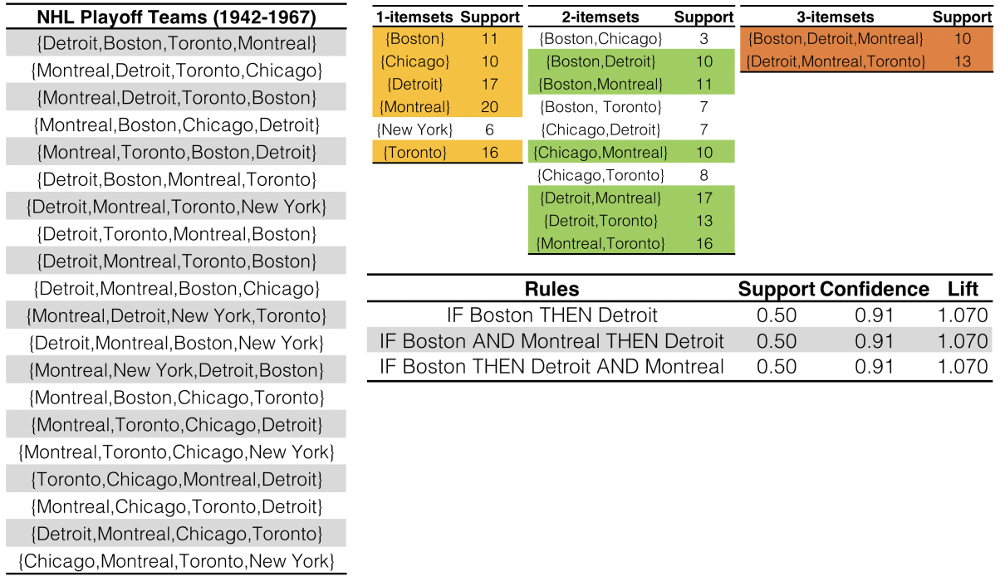
\includegraphics[width=\textwidth]{images/DSML/NHL.png}
\caption[\small Frequent item sets for NHL playoff teams.]{\small Association rules for NHL playoff teams (1942-1967). A list of the 4 teams making the playoffs each year is shown on the left ($N=20$). Frequent item sets are generated using the \textit{apriori} algorithms, with a support threshold of 10. We see that there are $5$ frequent 1-item sets, top row, in yellow (New York made the playoffs $6<10$ times -- no larger frequent item set can contain New York). 6 frequent 2-item sets are found in the subsequent list of ten 2-item sets, top row, in green (note the absence of New York). Only 2 frequent 3-item sets are found, top row, in orange. Candidate rules are generated from the shaded item sets; the rules retained by the thresholds $\textrm{Support}\geq 0.5$, $\textrm{Confidence}\geq 0.7$, and $\textrm{Lift}>1$ are shown in the table on the bottom row -- the main result is that when Boston made the playoffs, it was not surprising to see also Detroit make the playoffs (the presence or absence of Montreal in a rule is a red herring, as \textit{les Habitants} made the playoffs every year in the data.} \label{tab:NHL}\hrule
\end{table}
\begin{center}
    \rule{0.5\textwidth}{.4pt}
\end{center} 
As a more realistic example, consider the \textit{Titanic} dataset. Compiled by Robert Dawson in 1995, it consists of 4 categorical attributes for each of the 2201 people aboard the Titanic when it sank in 1912 (some issues with the dataset have been documented, but we will ignore them for now).  
\newpage\noindent \begin{figure}[!t]
\centering
\begin{subfigure}[b]{0.7\textwidth}
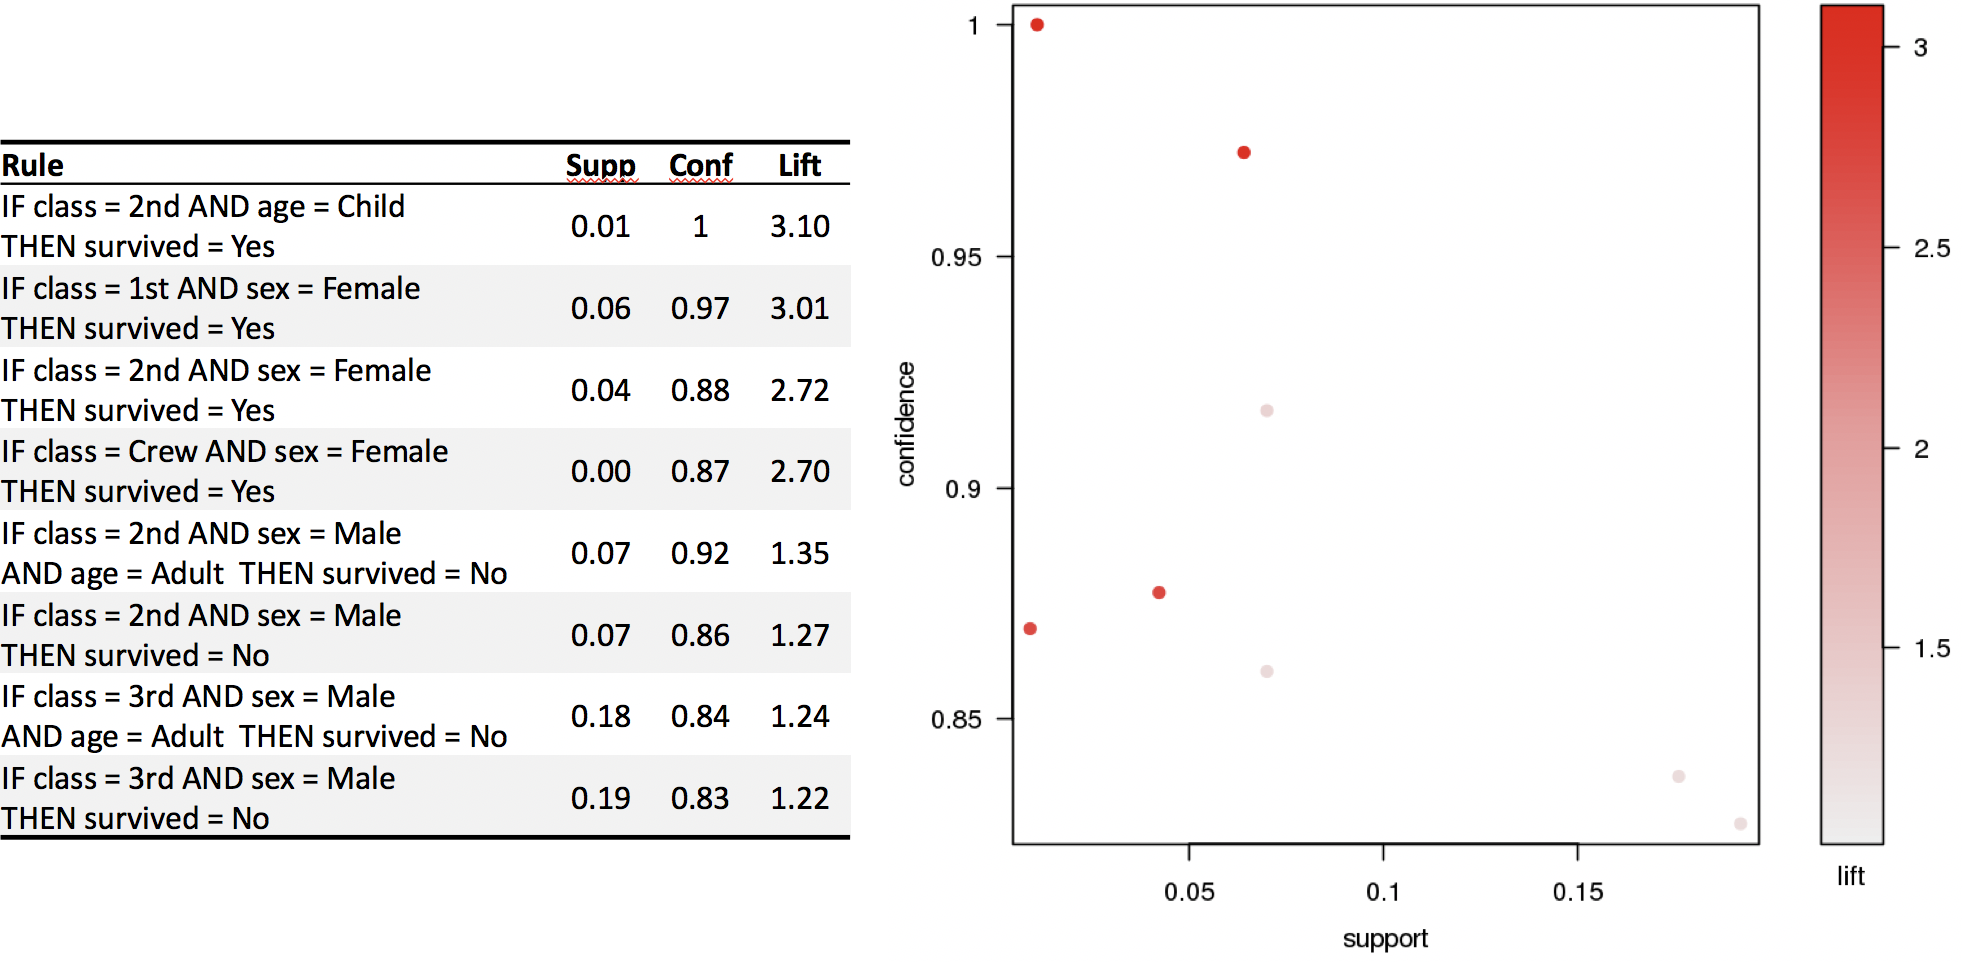
\includegraphics[width=\textwidth]{images/DSML/titanic1.png}\caption{\small Scatterplot} \label{fig:titanic1}
\end{subfigure}\qquad
\begin{subfigure}[b]{0.7\textwidth}
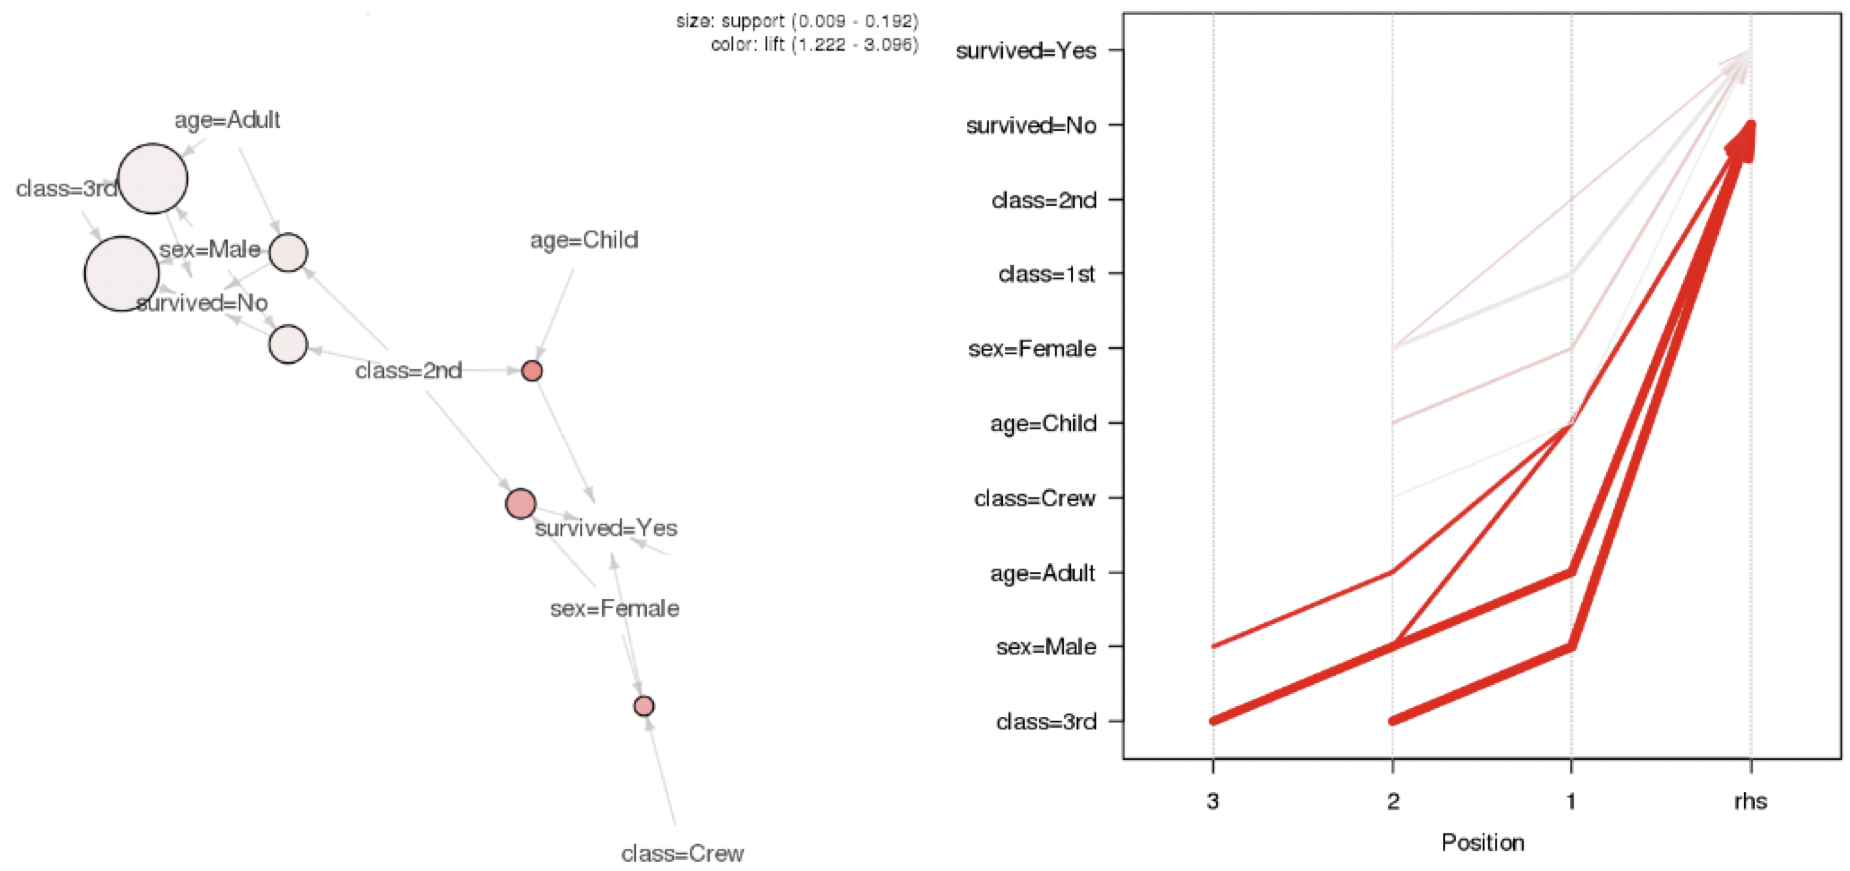
\includegraphics[width=\textwidth]{images/DSML/titanic2.png}\caption{\small Network and Parallel Coordinates} \label{fig:titanic2}
\end{subfigure}
\caption[\small Visualisations of the \textit{Titanic} association rules]{\small Visualisations of the 8 \textit{Titanic} association rules; scatterplot (top row), network diagram (bottom row, on the left), parallel coordinates (bottom row, on the right).}\label{fig:titanic}\hrule
\end{figure}\afterpage{\FloatBarrier}
The attributes/levels are:
\begin{itemize}[noitemsep]
\item \textbf{class} (first class, second class, third class, crewmember)
\item \textbf{age} (adult, child)
\item \textbf{sex} (male, female)
\item \textbf{survival} (yes, no)
\end{itemize}
The natural question of interest for this dataset is 
\begin{quote} how does survival relate to the other attributes? 
\end{quote} This is not, strictly speaking, an unsupervised task (as the interesting rules' structure is fixed to conclusions of the form $\textrm{survival} = \textrm{Yes}$ or $\textrm{survival} = \textrm{No}$); neither will we treat it as a predictive task (since the situation on the Titanic has little bearing on survival for new data). We will use fixed-structure association rules to \textbf{describe} explore the survival on the \textit{Titanic} (compare with \cite{DSML_MR}). 
We use the \texttt{arules} implementation of the \textit{apriori} algorithm in \texttt{R}  to generate and prune candidate rules, eventually leading to \textbf{8 rules} (the results can be visualised in Figure~\ref{fig:titanic}). Who survived? (As a final reminder, \textbf{correlation is still not causation}.)
\subsubsection{Supervised Learning and Classification}
\begin{tcolorbox}[title=An Embarrassment of Riches]
The diversity of problems that can be addressed by classification algorithms is significant, and covers many domains. [...] It is difficult to comprehensively discuss all the methods in a single book. \\[-0.6cm]
\begin{flushright}
-- C.C. Aggarwal, \textit{Data Classification: Algorithms and Applications}
\end{flushright}
\end{tcolorbox}
\noindent \textbf{Classification} is a supervised learning endeavour in which  a sample set of data (the \textbf{training} set) is used to determine rules and patterns that divide the data into predetermined groups, or classes. The training data usually consists of a \textbf{randomly} selected subset of the \textbf{labeled} data. \textbf{Value estimation} (regression) is similar to classification, except that the target variable is numerical. In the \textbf{testing phase}, the model is used to assign a class to observations for which the label is hidden, but ultimately known (the \textbf{testing} set).\newl  The performance of the predictive model is then evaluated by comparing the predicted and the values for the testing set observations (but \textbf{never} using the training set observations). A number of technical issues need to be addressed: which features to select for inclusion in the model and, perhaps more importantly, which algorithm to choose, for example. The mushroom (classification) model from earlier in this section is a good example of a classification model, although no detail were provided using the training data and choice of algorithm. 
\begin{center}
    \rule{0.5\textwidth}{.4pt}
\end{center} 
Classification and value estimation models are among the most frequently used of the data science models, and form the backbone of what is also known as \textbf{predictive analytics}. There are applications and uses in just about every field of human endeavour, such as: 
\begin{itemize}[noitemsep]
\item \textbf{medicine and health science} -- predicting which patient is at risk of suffering a second, and this time fatal, heart attack within 30 days based on health factors (blood pressure, age, sinus problems, etc.);
\item \textbf{social policies} -- predicting the likelihood of required assisting housing in old age based on demographic information/survey answers;
\item \textbf{marketing and business} -- predicting which customers are likely to cancel their membership to a gym based on demographics and usage; 
\item in general, predicting that an object belongs to a particular class, or organising and grouping instances into categories, or 
\item enhancing the detection of relevant objects: 
\begin{itemize}[noitemsep,topsep=2pt]
\item \textbf{avoidance} -- ``this object is an incoming vehicle''; \item \textbf{pursuit} -- ``this borrower is unlikely to default on her mortgage''; \item \textbf{degree} -- ``this dog is 90\% likely to live until it's 7 years old''. 
\end{itemize}
\end{itemize}
Other examples may be found in \cite{DSML_CS1,DSML_CS2,DSML_CS3,DSML_CS4}. 
\newpage\noindent 
Some concrete examples may provide a clearer picture of the types of supervised learning problems that quantitative consultants may be called upon to solve.  
\begin{itemize}[noitemsep]
\item A motor insurance company has a fraud investigation department that studies up to 20\% of all claims made, yet money is still getting lost on fraudulent claims. To help better direct the investigators, management would like to determine, using past data, if it is possible to predict 
\begin{itemize}[noitemsep,topsep=2pt]
\item whether a claim is likely to be fraudulent? 
\item whether a customer is likely to commit fraud in the near future?
\item whether an application for a policy is likely to result in a fraudulent claim?
\item the amount by which a claim will be reduced if it is fraudulent? 
\end{itemize}
What kind and how much data do you think is required? What would constitute a predictive success? How would you help the client understand these risks associated with a predictive modeling approach? 
\item Customers who make a large number of calls to a mobile phone company's customer service number have been identified as churn risks. The company is interested in reducing said churn. Can they predict
\begin{itemize}[noitemsep,topsep=2pt]
\item the overall lifetime value of a customer? 
\item which customers are more likely to churn in the near future? 
\item what retention offer a particular customer will best respond to?
\end{itemize}
How would you use standard statistical techniques to answer these questions?
\end{itemize}
\begin{center}
    \rule{0.5\textwidth}{.4pt}
\end{center}
In the absence of testing data, classification models cannot be used for predictive tasks, but may still be useful for \textbf{descriptive} tasks. When testing data exists, the process is often quite similar, independently of the choice of the algorithm (see the classification pipeline shown in Figure~\ref{fig:class1}). 
\begin{figure}[!t]
\centering
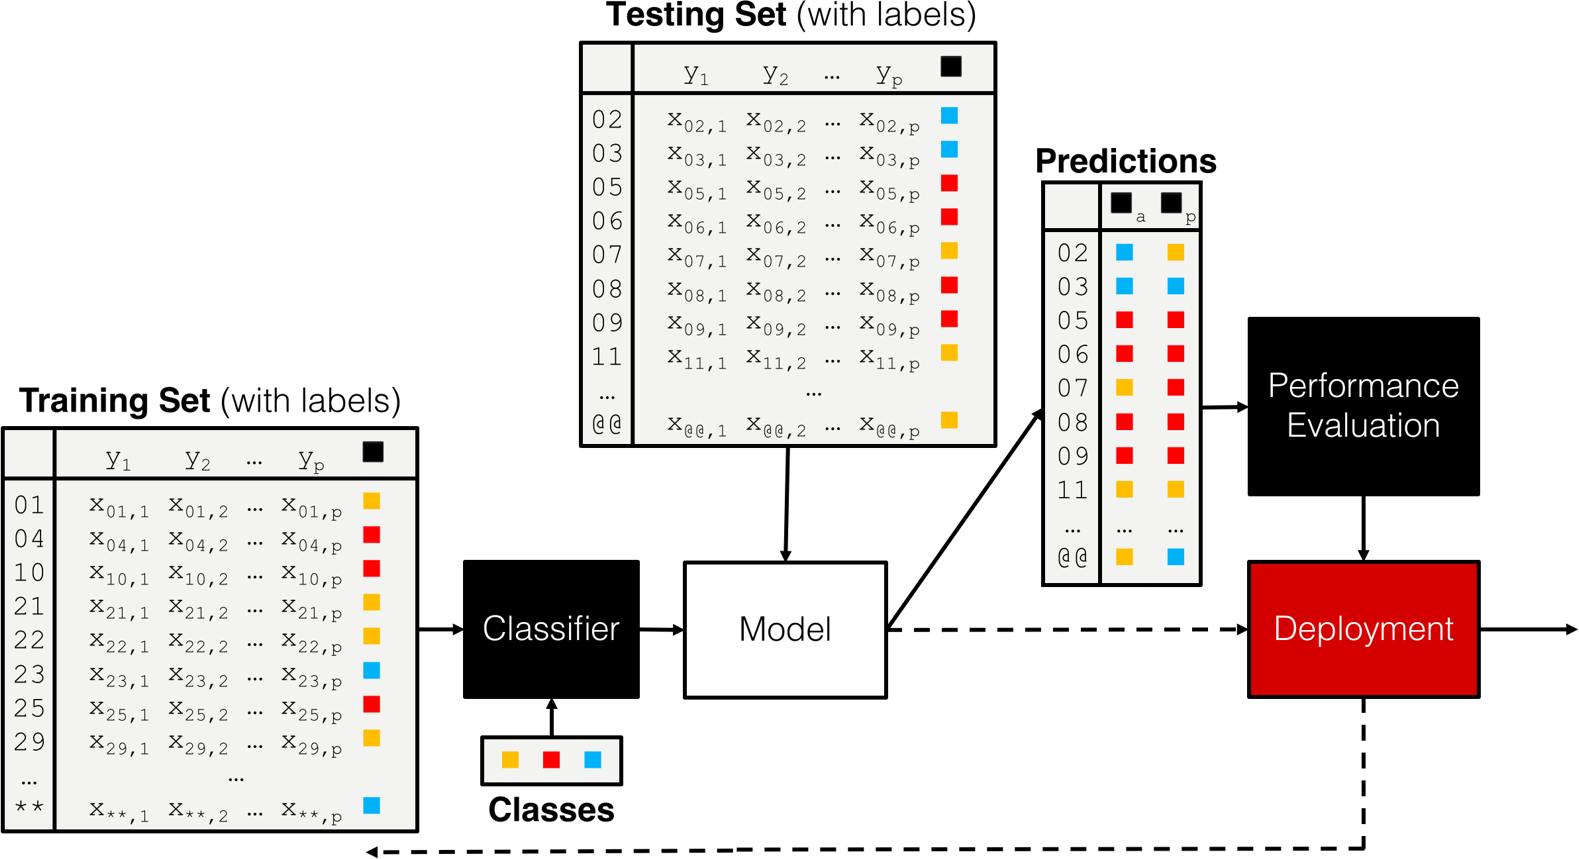
\includegraphics[width=\textwidth]{images/DSML/Classifer_Pipeline.png}
\caption[\small Classification pipeline]{\small A classification pipeline, including training set, testing set, performance evaluation, and (eventual) deployment.}\label{fig:class1}
\end{figure}
\afterpage{\FloatBarrier}
\paragraph{Classification Algorithms}
The number of classification algorithms is truly staggering -- it often seems as though new algorithms and variants are put forward on a monthly basis, depending on the task and on the type of data \cite{DSML_CS10}. Here are common algorithms that data scientists should have at their command (full descriptions available in \cite{DSML_T,DSML_HTF,DSML_PF}): 
\begin{figure}[!t]
\centering
\begin{subfigure}[b]{0.45\textwidth}
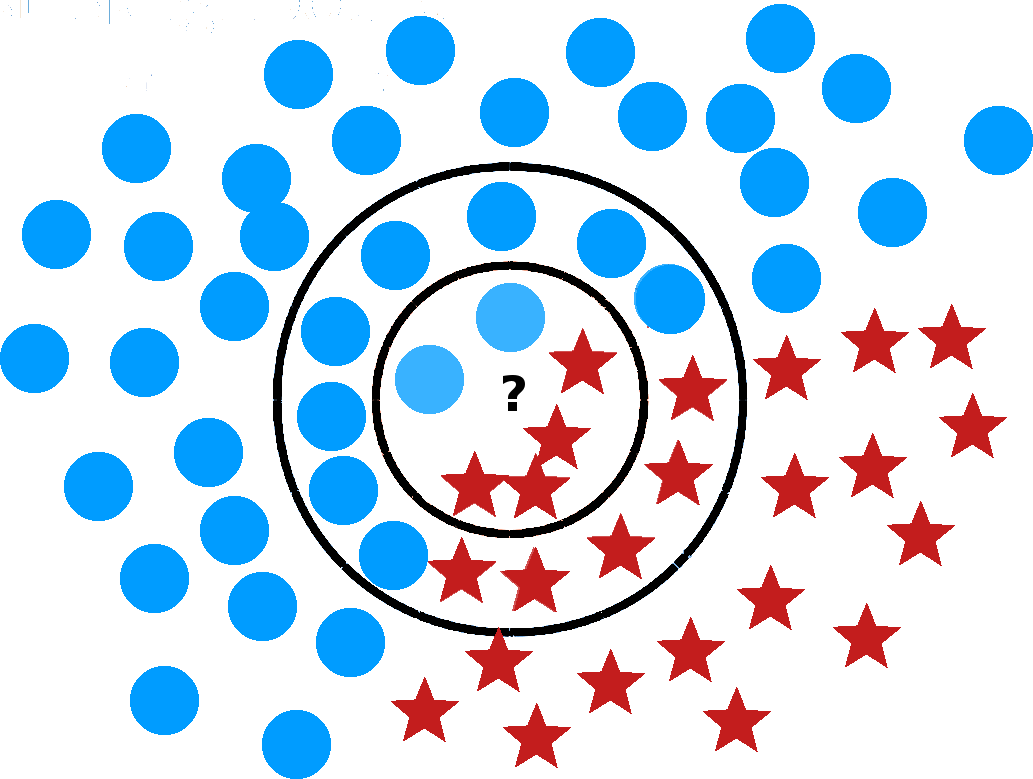
\includegraphics[height=0.25\textheight]{images/DSML/knn.png}
\caption{\small $k$NN}\label{fig:class2a}
\end{subfigure}
\begin{subfigure}[b]{0.45\textwidth}
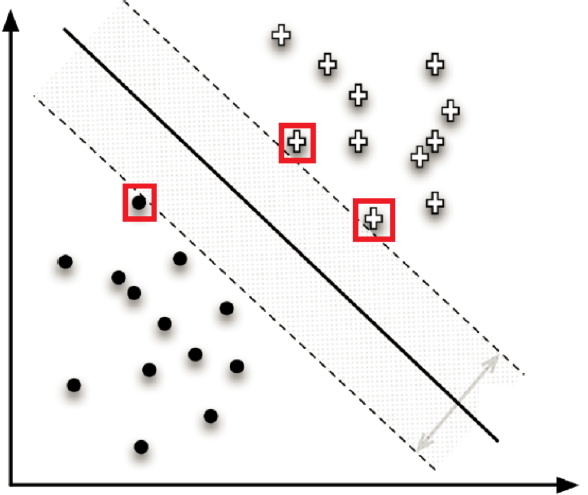
\includegraphics[height=0.25\textheight]{images/DSML/SVM.png}
\caption{\small SVM}\label{fig:class2b}
\end{subfigure}
\caption[\small Illustration of $k$NN and SVM]{\small Illustration of a $k$ nearest neighbour (left) and a support vector machines classifier (right, based on \cite{DSML_PF}). What is the 6NN prediction for the location marked by a question mark? What about the 19NN prediction? }\label{fig:class2}
\end{figure}
\afterpage{\FloatBarrier}
\begin{figure}[!t]
\centering
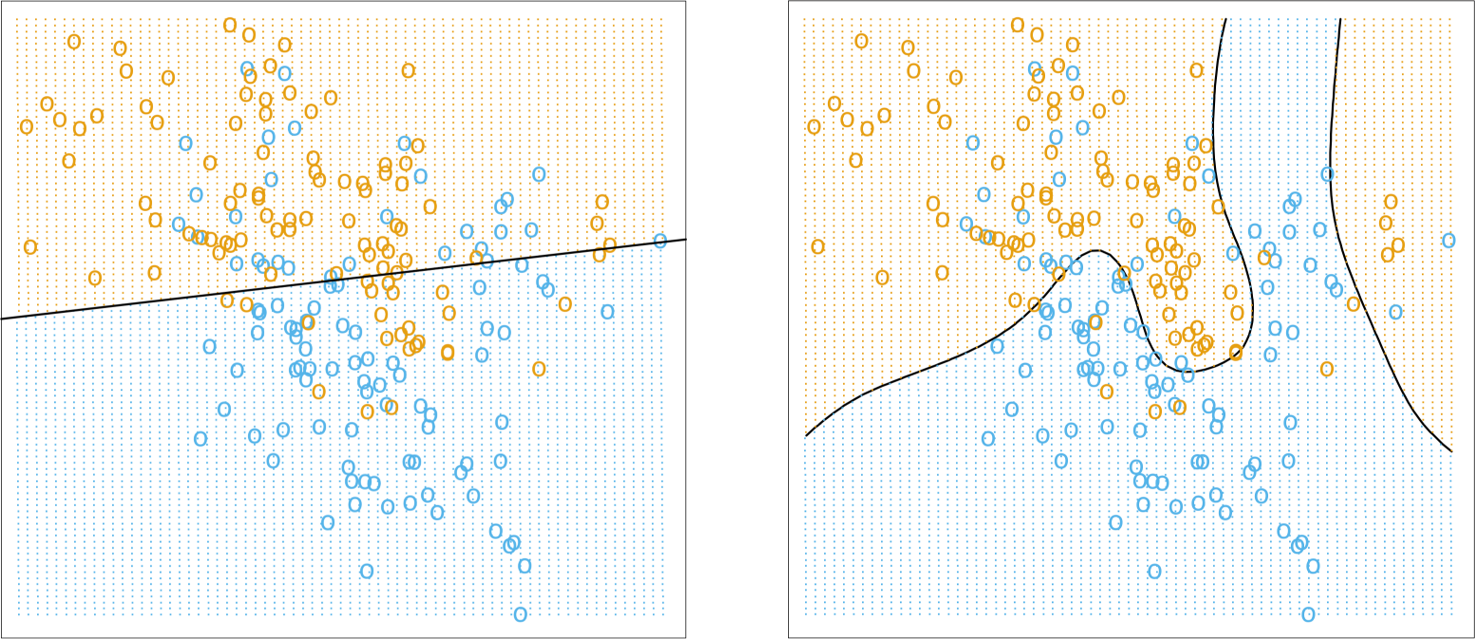
\includegraphics[width=0.8\textwidth]{images/DSML/illustration1.png}
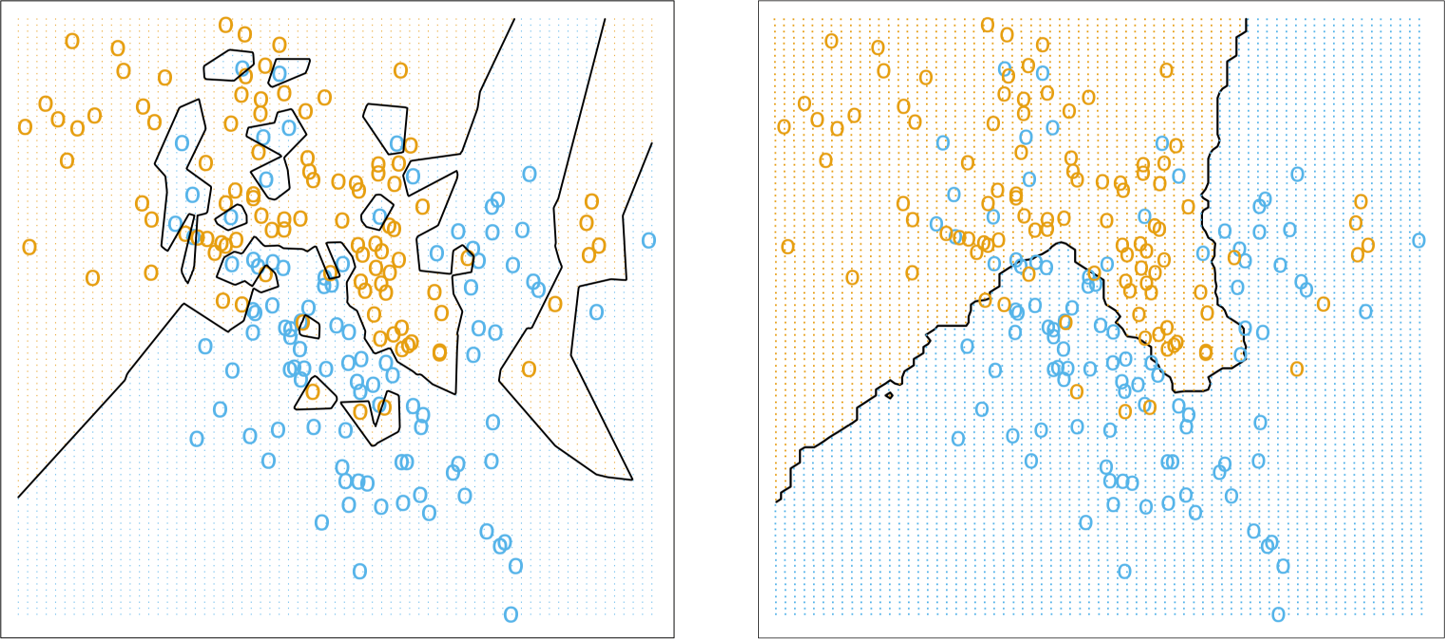
\includegraphics[width=0.8\textwidth]{images/DSML/illustration2.png}
\caption[\small Illustrations of linear regression, optimal Bayes, and $k$NN]{\small Illustrations of various classifiers (linear regression, top left; optimal Bayes (top right); 1NN and 15NN (bottom left and right, respectively) on an artificial dataset (from \cite{DSML_HTF}). Note that linear regression is more stable, simpler to describe, and less accurate than $k$NN and optimal Bayes.}\label{fig:class3}
\end{figure}
\afterpage{\FloatBarrier}
\begin{figure}[!t]
\centering
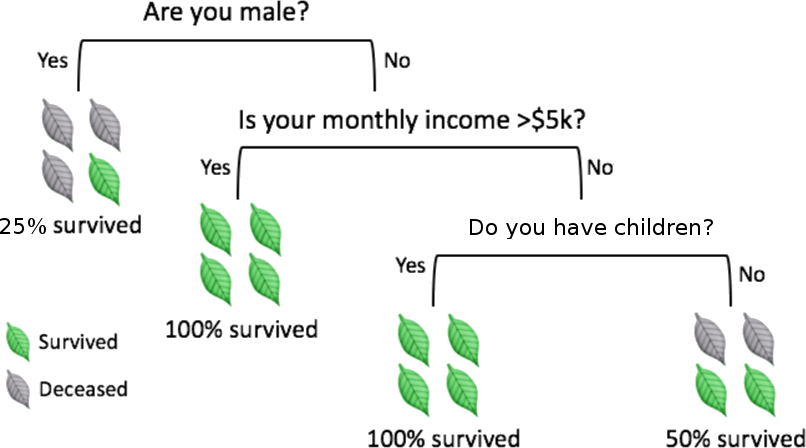
\includegraphics[width=0.8\textwidth]{images/DSML/tree_example.png}
\caption[\small Illustration of a decision tree]{\small Illustration of a decision tree depicting the chances of survival for various disasters (fictional, based on \cite{DSML_NS}).}\label{fig:class4}
\end{figure}
\afterpage{\FloatBarrier}
\begin{itemize}[noitemsep]
\item \textbf{logistic regression} and linear regression are classical models which are often used by statisticians but rarely in a classification setting (the estimated coefficients are often used to determine the features' importance); one of their strengths is that the machinery of standard statistical theory (hypothesis testing, confidence intervals, etc.) is still available to the analyst, but they are easily affected by variance inflation in the presence of predictor multi-colinearity, and the stepwise variable selection process that is typically used is problematic -- regularisation methods would be better suited \cite{DSML_LASSO} (see Figure~\ref{fig:class3}, top left);
\item \textbf{neural networks} have become popular recently due to the advent of deep learning; they might provide the prototypical example of a \textbf{black box} algorithm as they are hard to interpret; another issue is that they require a fair amount of data to train properly -- we will have more to say on the topic in a later section; 
\item \textbf{decision trees} are perhaps the most commons of all data science algorithms, but they tend to overfit the data when they are not pruned correctly (a process which often has to be done manually) -- we will provide a bit more details shortly (see Figure~\ref{fig:class4}); 
\item \textbf{na\"{\i}ve Bayes classifiers} have known quite a lot of success in text mining applications (more specifically as the basis of powerful spam filters), but, embarrassingly, no one is quite sure why they should work as well as they do given that one of their required assumptions (independence of priors) is rarely met in practice (see Figure~\ref{fig:class3}, top right);
\item \textbf{support vector machines} attempt to separate the dataset by ``fitting'' as wide of a ``tube'' as possible through the classes (subjected to a number of penalty constraints); they have also known successes, most notably in the field of digital handwriting recognition, but their decision boundaries (the tubes in question) tend to be non-linear and quite difficult to interpret; nevertheless, they may help mitigate some of the difficulties associated with big data (see Figure~\ref{fig:class2a});
\item \textbf{nearest neighbours classifiers} basically implement a voting procedure and  require very little assumptions about the data, but they are not very stable as adding training points may substantially modify the boundary (see Figures~\ref{fig:class2a} and \ref{fig:class3}, bottom row)).
\end{itemize}
\paragraph{Decision Trees}
Decision trees are perhaps the most \textbf{intuitive} of these methods: classification is achieved by following a path up the tree, from its \textbf{root}, through its \textbf{branches}, and ending at its \textbf{leaves} (alghough typically the tree is depicted with its root at the top and its leaves at the bottom). \par To make a \textbf{prediction} for a new instance, it suffices to follow the path down the tree, reading the prediction directly once a leaf is reached. It sounds simple enough in theory, but in practice, creating the tree and traversing it might be \textbf{time-consuming} if there are too many variables in the dataset (due to the criterion that is used to determine how the branches split). 
\par Prediction accuracy can be a concern in trees whose growth is \textbf{unchecked}. In practice, the criterion of \textbf{purity} at the leaf-level (that is to say, all instances in a leaf belong to the same leaf) is linked to bad prediction rates for new instances. Other criteria are often used to prune trees, which may lead to impure leaves.
\begin{center}
    \rule{0.5\textwidth}{.4pt}
\end{center} 
How do we grow such trees? For predictive purposes, we need a training set and a testing set upon which to evaluate the tree's performance. Ross Quinlan's \textbf{Iterative Dichotomizer 3} (a precursor to his widely-used C4.5) follows a simple path: 
\begin{enumerate}[noitemsep]
\item split the training data (\textbf{parent}) set into (\textbf{children}) subsets, using the different levels of a particular attribute;
\item compute the \textbf{information gain} for each subset;
\item select the \textbf{most advantageous} split, and 
\item repeat for each node until some \textbf{leaf criterion} is met. 
\end{enumerate}
\textbf{Entropy} is a measure of disorder in a set $S$. Let $p_i$ be the proportion of observations in $S$ belonging to category $i$, for $i=1,\ldots, n$. The entropy of $S$ is given by $$E(S)=-\sum_{i=1}^n p_i\log p_i.$$
If the \textbf{parent set} $S$ consisting of $m$ records is split into $k$ children sets $C_1,\ldots, C_k$ containing $q_1, \ldots, q_k$ records, respectively, then the \textbf{information gained} from the split is  
$$I(S:C_1,\ldots,C_k)=E(S)-\frac{1}{m}\sum_{j=1}^kq_jE(C_j).$$
The second term on the right-hand side of the information gain equation is a weighted average of the entropy of the children sets. If the split leads to little disorder in the children, then $\textrm{IG}(S;C_1,\ldots,C_k)$ is high; if the split leads to similar disorder in both children and parent, then $\textrm{IG}(S;C_1,\ldots,C_k)$ is low.\par Consider, for instance, two splits shown for a parent set with 30 observations separated into 2 classes: $\circ$ and $\star$ (as in Figure~\ref{fig:class5}).   
\begin{figure}[!t]
\centering
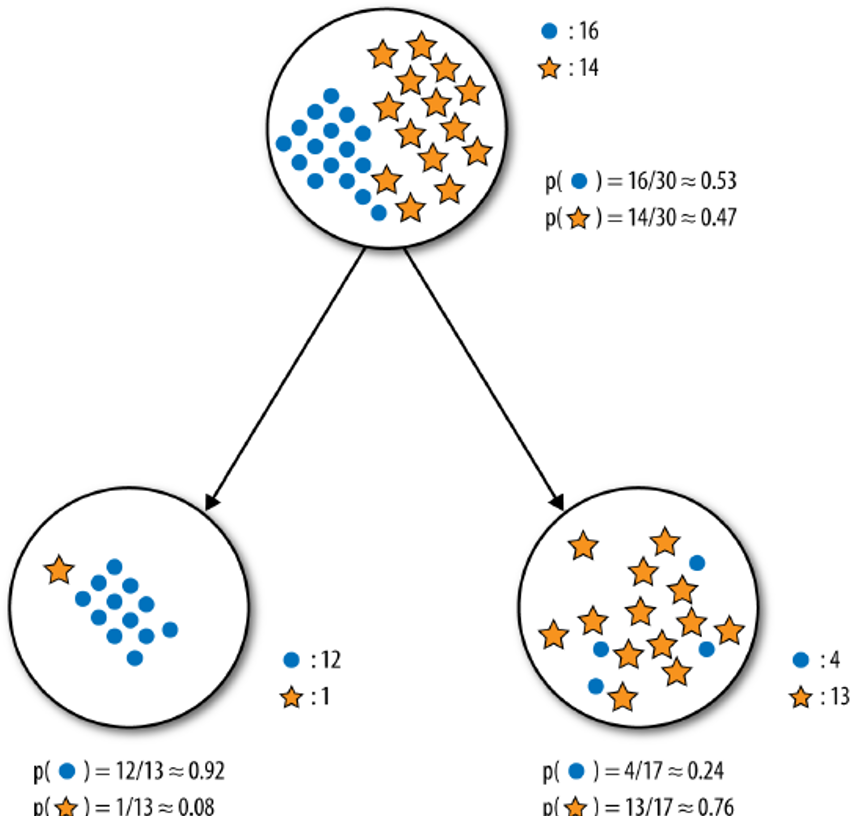
\includegraphics[height=0.3\textheight]{images/DSML/parentchildren1.png}
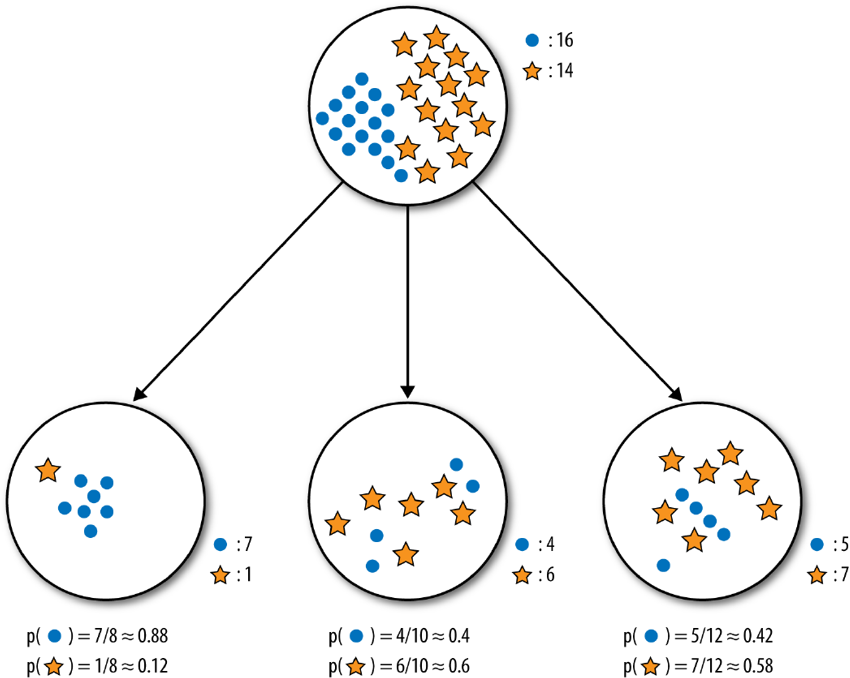
\includegraphics[height=0.3\textheight]{images/DSML/parentchildren2.png}
\caption[\small Picking the optimal information gain split]{\small Picking the optimal information gain split (from \cite{DSML_PF}).}\hrule\label{fig:class5}
\end{figure}
\afterpage{\FloatBarrier}
Visually, it appears as though the binary split does a better job of separating the classes. Numerically, the entropy of the parent set $S$ is $$E(S)=-p_{\circ}\log p_{\circ} - p_{\star}\log p_{\star}=-\frac{16}{30}\log \frac{16}{30} - \frac{14}{30}\log \frac{14}{30} \approx 0.99.$$ For the binary split (on the left), leading to the children set $L$ (left) and $R$ (right), the respective entropies are 
$$E(L)=-\frac{12}{13}\log \frac{12}{13} - \frac{1}{13}\log \frac{1}{13} \approx 0.39 $$ and 
$$E(R)=-\frac{4}{17}\log \frac{4}{17} - \frac{13}{17}\log \frac{13}{17} \approx 0.79,$$
so that the information gained by that split is 
$$\textrm{IG}(S;C_L,C_R)\approx 0.99-\frac{1}{30}\left[13\cdot 0.39+17\cdot 0.79\right]=0.37.$$ On its own, this value is not substantially meaningful -- it is when compared with the information gained from other splits that it becomes useful. 
A similar computation for the the ternary split leads to $\textrm{IG}(S;C_1,C_2,C_3)\approx 0.13$, which is indeed smaller than the information gained by the binary split -- given those two choices, ID3 would select the first split as being \textbf{most advantageous}. \newpage\noindent
Decision trees have numerous strengths: they 
\begin{itemize}[noitemsep]
\item are easy to interpret, providing, as they do, a \textbf{white box model} -- predictions can always be explained by following the appropriate paths;
\item can handle numerical and categorical data \textbf{simultaneously}, without first having to ``binarise'' the data;
\item can be used with \textbf{incomplete} datasets, if needed (being some of the algorithms with that property, although there is still some value in imputing missing observations);
\item allow for \textbf{built-in feature selection} in that less relevant features do not typically tend to be used as splitting features; 
\item make \textbf{no assumption} about independence of observations, underlying distributions, multi-colinearity, etc., and can thus be used without the need to verify assumptions; 
\item lend themselves to \textbf{statistical validation} (in the form of cross-validation), and 
\item are in line with \textbf{human decision-making approaches}, especially when such decisions are taken deliberately.
\end{itemize}
On the other hand, they are 
\begin{itemize}[noitemsep]
\item \textbf{not usually as accurate} as other more complex algorithms, nor \textbf{as robust}, as small changes in the training data can lead to a completely different tree, with a completely different set of predictions (this can be problematic when presenting the results to a client whose understanding of these matters is slight);
\item particularly \textbf{vulnerable to overfitting} in the absence of pruning -- and pruning procedures are typically fairly convoluted (some models, such as conditional inference trees, automate this process, using statistical tests to determine when a tree's ``full'' growth has been achieved), and
\item \textbf{biased} towards categorical features with high number of levels, which may give such variables undue importance in the classification process.
%Optimal decision tree learning is NP-complete
\end{itemize}
Information gain tends to grow small trees in its puruit of pure leaves, but is not the only splitting metric in use -- common alternatives include \textbf{Gini impurity} and \textbf{variance reduction}. As mentioned previously, ID3 is a precursor of C4.5, perhaps the most popular decision tree algorithm on the market. There are other tree algorithms, such as C5.0, CHAID, MARS, conditional inference trees, CART, etc., each grown using algorithms with their own strengths and weaknesses. \newl Decision trees can also be combined together using \textbf{boosting algorithms} (such as \textit{AdaBoost}) or \textbf{random forests}, providing a type of voting procedure also known as \textbf{ensemble learning} -- an individual tree might make middling predictions, but a large number of them are likely to make good predictions, on average. 
\newl There are still a few other points to ponder on the topic of decision trees;
\begin{itemize}[noitemsep]
\item since classification is linked to probability estimation, approaches that extend the basic ideas of regression models could prove fruitful;
\item rare occurrences are often more interesting and more difficult to predict and identify than regular instances -- historical data at Fukushima's nuclear reactor prior to the 2011 meltdown could not have been used to learn about meltdowns, for obvious reasons (classical performance evaluation metrics can easily be fooled; if out of two classes one of the instances is only represented in 0.01\% of the instances, predicting the non-rare class will yield correct predictions roughly 99.99\% of the time, missing the point of the exercise altogether;
\item with big datasets, algorithms must also consider efficiency -- thankfully, decision trees are easily parallelisable. 
\end{itemize}
\begin{center}
    \rule{0.5\textwidth}{.4pt}
\end{center} 
\textbf{IMPORTANT NOTE:} as a consequence of the (so-called) \textbf{No-Free-Lunch Theorem}, no single classifier can be the best performer for every problem. The model selection process must take into consideration the nature of the available data, the relative frequencies of the classification sub-groups and the stated goals of the classification. Other considerations may include how easily the model lends itself to interpretation and statistical analysis; how much data preparation it requires; whether it can accommodate various data types and missing observations; whether it performs well with large datasets, and whether it is robust against small data departures from theoretical assumptions. The client might not be aware that past success is not a guarantee of future success -- it is your responsibility to ensure that you try out various models.  
\begin{center}
    \rule{0.5\textwidth}{.4pt}
\end{center} \paragraph{Performance Evaluation}
When a classifier attempts to determine what kind of music a new customer would prefer, there is next to no cost in making a mistake; if, on the other hand, the classifier attempts to determine the presence or absence of cancerous cells in lung tissue, mistakes are somewhat more unforgivable. Several metrics can be used to assess a classifier's performance, depending on the context. \par \textbf{Binary classifiers} (such as the abstract example shown in Table~\ref{tab:binary_class}) are simpler and have been studied far longer than multi-level classifiers; consequently, a larger body of evaluation metrics is available for these classifiers. 
\begin{table}[!t] \begin{center}
    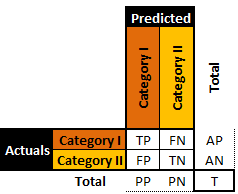
\includegraphics[width=0.45\textwidth]{images/DSML/binary_classifier}
  \end{center}
  \caption{\small A general binary classifier.}\hrule
  \label{tab:binary_class}
\end{table}
In the medical literature, $\textrm{TP}$, $\textrm{TN}$, $\textrm{FP}$ and $\textrm{FN}$ stand for \textit{True Positives}, \textit{True Negatives}, \textit{False Positives}, and \textit{False Negatives}, respectively. A perfect classifier would be one for which both $\textrm{\textrm{FP}},\textrm{FN}=0$. In practice, that rarely ever h\textrm{AP}pens (if at all).\newpage\noindent \begin{table}[!t]
  \begin{center}
    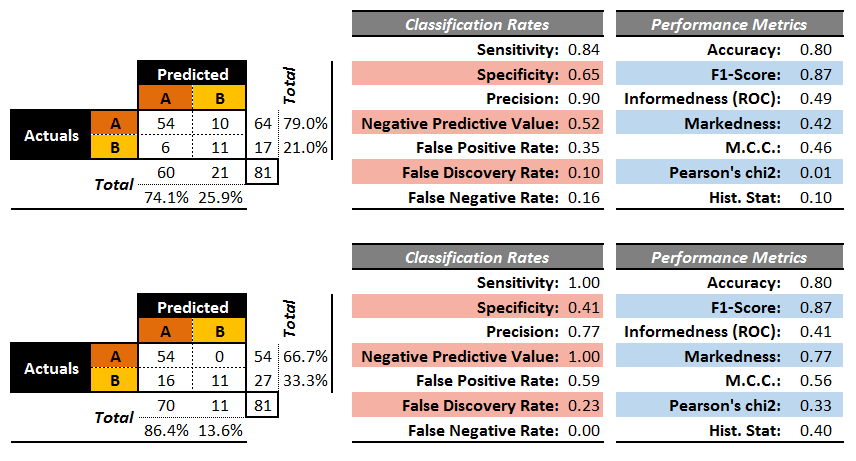
\includegraphics[width=\textwidth]{images/DSML/Classification_Performance_Metrics}
  \end{center}
  \caption{\small Performance metrics for two (artificial) binary classifiers.}\hrule
  \label{tab:bin_perf_metrics}
\end{table}
Traditional performance metrics include: 
\begin{itemize}[noitemsep] \item {Sensitivity:} $\textrm{TP}/\textrm{AP}$ \item {Specificity:} $\textrm{TN}/\textrm{AN}$ \item {Precision:} $\textrm{TP}/\textrm{PP}$ \item {Negative Predictive Value:}   $\textrm{TN}/\textrm{PN}$ \item {False Positive Rate:} $\textrm{FP}/\textrm{AN}$ \item {False Discovery Rate:} $1-\textrm{TP}/\textrm{PP}$\item {False Negative Rate:} $\textrm{FN}/\textrm{AP}$ \item {Accuracy:} $(\textrm{TP}+\textrm{TN})/\textrm{T}$ \item {$F_1-$Score:} $2\textrm{TP}/(2\textrm{TP}+\textrm{FP}+\textrm{FN})$\item  {MCC:}  $(\textrm{TP}\cdot \textrm{TN}-\textrm{FP}\cdot \textrm{FN})(\textrm{AP}\cdot \textrm{AN}\cdot \textrm{PP} \cdot \textrm{PN})^{-1/2}$\item {Informedness/ROC:} $\textrm{TP}/\textrm{AP}+\textrm{TN}/\textrm{AN}-1$ \item {Markedness:} $\textrm{TP}/\textrm{PP}+\textrm{TN}/\textrm{PN}-1$
\end{itemize}  
The \textbf{confusion matrices} of two artificial binary classifers are shown in Table~\ref{tab:bin_perf_metrics}. Both classifiers have an accuracy of $80\%$, but the classifiers are not of the same quality: while the second classifier sometimes makes a wrong prediction for $A$, it never makes one for $B$, whereas the first classifier makes wrong predictions for both $A$ and $B$. On the other hand, the second classifier mistakenly predicts occurrence $A$ as $B$ 16 times while the first one only does so 6 times. \par So which one is best? The performance metrics alone do not suffice to answer the question: a lot depends on the price associated with making a mistake. There's a good reason to use the Mathews Correlation Coefficient: of all the performance metrics, only it and the accuracy easily generalize to multi-level classifiers.  
\newpage\noindent \textbf{Accuracy} is the proportion of correct predictions amid all the observations; its value ranges from 0\% to 100\%. The higher the accuracy, the better the match, and yet, a predictive model with high accuracy may nevertheless be useless thanks to the \textit{Accuracy Paradox} (this is especially problematic when one of the categories contains substantially fewer members than the others). The 
\textbf{Matthews Correlation Coefficient} (MCC), on the other hand,  is a statistic which is of use even when the classes are of very different sizes. As a correlation coefficient  between the actual and predicted classifications, its range varies from $−1$ to $1$. If $\textrm{MCC}=1$, the predicted and actual responses are identical, while if $\textrm{MCC}=0$, the classifier performs no better than a random prediction (``flip of a coin''). It is also possible to introduce two non-traditional performance metrics (which are nevertheless well-known statistical quantities) to describe how accurately a classifier preserves the classification distribution (rather than how it behaves on an observation-by-observation basis):
\begin{itemize}[noitemsep]
\item Pearson's $\chi^2$: $\frac{1}{\textrm{T}}\left((\textrm{PP}-\textrm{AP})^2/\textrm{PP} + (\textrm{PN}-\textrm{AN})^2/\textrm{PN}\right)$ 
\item Hist: $\frac{1}{\textrm{T}}\left(\left|\textrm{PP}-\textrm{AP}\right|+\left|\textrm{PN}-\textrm{AN}\right|\right)$
\end{itemize}
For a given number of levels, the smaller these quantities, the more similar the actual and predicted distributions (see Tables~\ref{tab:ternary} for examples of confusion matrices for multi-level classifiers). \par For numerical targets $y$
\begin{table}[t]
  \centering
  \begin{subtable}[c]{0.4\textwidth}
    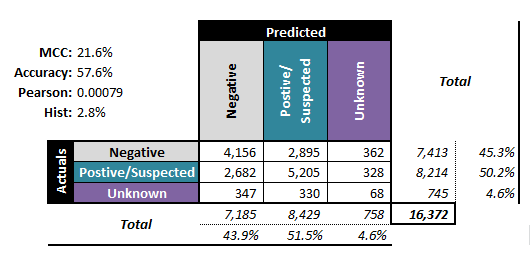
\includegraphics[width=1\textwidth]{images/DSML/confusion_bonus_50run_noinfo_rep}
  \caption{\small Ternary classifier.}
  \end{subtable}
    \begin{subtable}[c]{0.45\textwidth}
    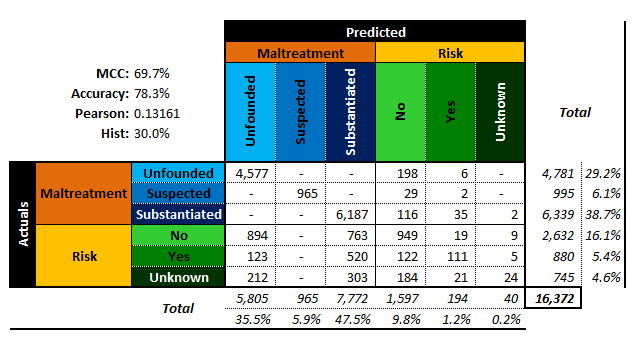
\includegraphics[width=1\textwidth]{images/DSML/confusion_classification_50run_info}
  \caption{\small Senary classifier.}
  \end{subtable}
  \caption{\small Performance metrics for (artificial) multi-level classifiers.}\hrule
  \label{tab:ternary}
\end{table}
 with predictions $\hat{y}$, the confusion matrix is not applicable, but a number of classical performance evaluation metrics are used: the 
\begin{itemize}[noitemsep]
\item mean squared and mean absolute errors $$\textrm{MSE}=\textrm{mean}\left\{(y_i-\hat{y}_i)^2\right\}, \quad \textrm{MAE}=\textrm{mean}\{|y_i-\hat{y}_i|\};$$ 
\item normalised mean squared and mean absolute errors $$\textrm{NMSE}=\frac{\textrm{mean}\left\{(y_i-\hat{y}_i)^2\right\}}{\textrm{mean}\left\{(y_i-\overline{y})^2\right\}},\quad \textrm{NMAE}=\frac{\textrm{mean}\left\{|y_i-\hat{y}_i|\right\}}{\textrm{mean}\left\{|y_i-\overline{y}|\right\}};$$
\item mean average percentage error $$\textrm{MAPE}=\textrm{mean}\left\{\frac{|y_i-\hat{y}_i|}{y_i}\right\};$$
\item correlation $\rho_{y,\hat{y}}$.
\end{itemize}
An isolated performance metric does not provide enough of a rationale for model validation, unless it has first been normalised. There is much more to be said on the topic of model selection, but that is outside the scope of this document.  
\newpage\noindent As a basic illustration
\begin{figure}[!t]
\centering
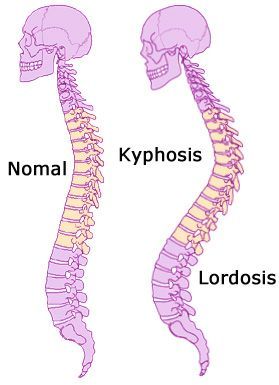
\includegraphics[width=0.3\textwidth]{images/DSML/kyphosis.png}
\caption[\small Kyphosis (medical condition)]{\small Kyphosis (medical condition). Surgery may cure the condition in children, but the procedure is not without risk. Are there factors that can determine if it is likely to be succesful prior to conducting it?}\hrule\label{fig:class6}
\end{figure}
\afterpage{\FloatBarrier}
of these concepts, consider the following example. \textbf{Kyphosis} is a medical condition related to an excessive convex curvature of the spine. Corrective spinal surgery is at times performed on children. A dataset of 81 observations and 4 attributes has been collected  (we have no information on how the data was collected and how representative it is likely to be, but those details can be gathered from \cite{DSML_HC}).  The attributes are:
\begin{itemize}[noitemsep]
\item \textbf{kyphosis} (absent or present after presentation)
\item \textbf{age} (at time of operation, in months)
\item \textbf{number} (of vertebrae involved)
\item \textbf{start} (topmost vertebra operated on)
\end{itemize}
The question of interest for this natural dataset is 
\begin{quote} how do the three explanatory attributes impact the operation's success?
\end{quote} 
We use the \texttt{rpart} implementation of CART in \texttt{R} to generate some decision trees (strictly speaking, this is not a predictive supervised task as we treat the entire dataset as a training set for the time being -- there are no hold-out testing observations). The results are shown in Figure~\ref{fig:class7}. Interestingly, it would appear that the \texttt{number} variable does not play a role in determining the success of the operation (for the observations in the dataset). 
\begin{figure}[!t]
\centering
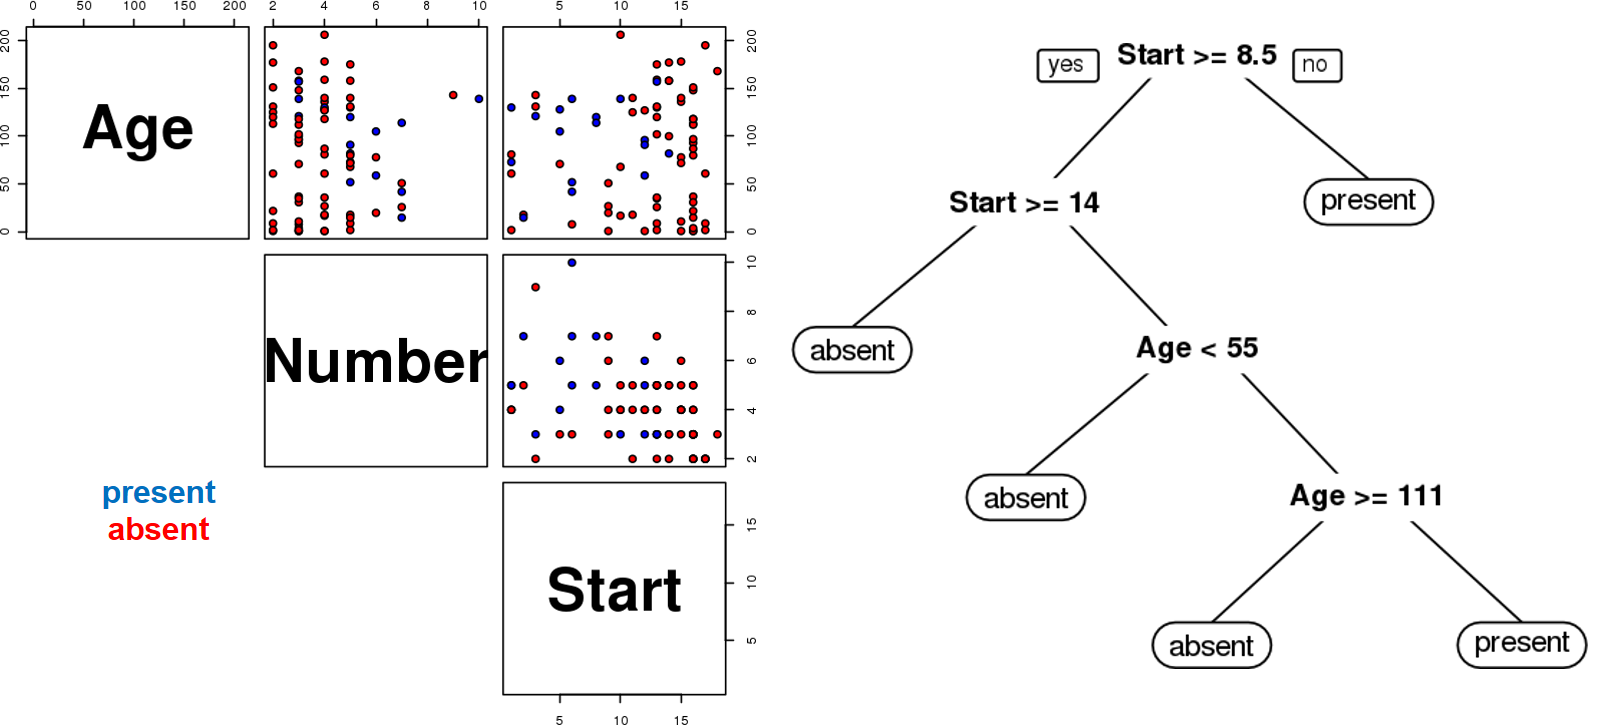
\includegraphics[width=0.9\textwidth]{images/DSML/kyphosis1.png}
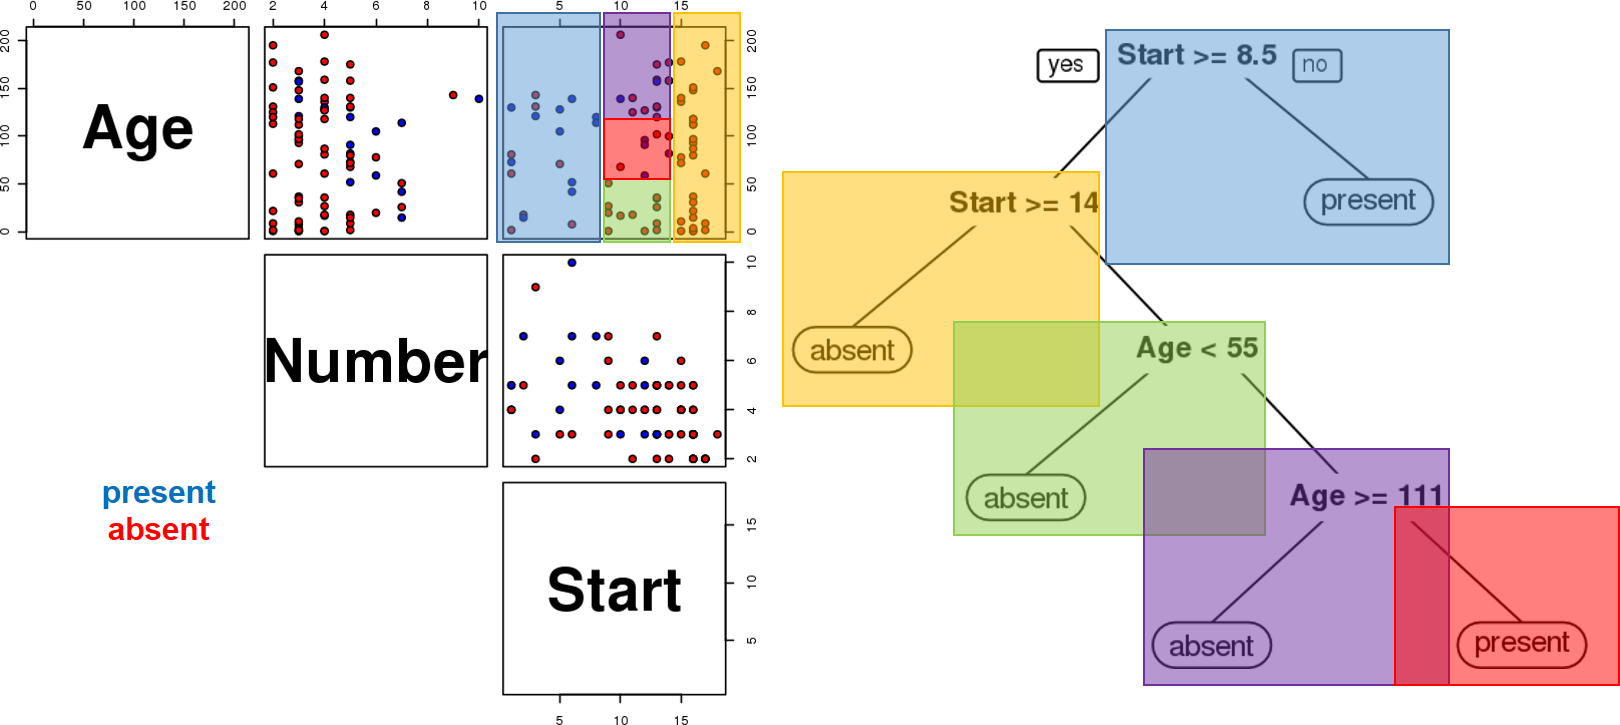
\includegraphics[width=0.9\textwidth]{images/DSML/kyphosis2.png}
\caption[\small Kyphosis decision tree -- visualisation]{\small Kyphosis decision tree -- visualisation. Only two features are used to construct the tree. We also note that the leaves are not pure -- there are blue and red instances in 3 of the 5 classification regions.}\label{fig:class7}
\end{figure}
\afterpage{\FloatBarrier}
\par The visualisation of the decision tree certainly indicates that its leaves are not pure; more details can be found in a slightly different visualisation (see Figure~\ref{fig:class8a}). A bit more (off-page) work suggests that the tree is somewhat overgrown and that it could benefit from being pruned after the first branching point (see Figure~\ref{fig:class8b}). At any rate, it is mostly meaningless to discuss the performance of the tree if we are not using a holdout testing sample (not to say anything about the hope of generalising to a larger population). To that end, we trained a model on 50 randomly selected observations and evaluated the performance on the remaining 31 observations (the structure of the tree is not really important at this stage). The results are shown in Table~\ref{fig:class9}. Is this a good model? 
\begin{figure}[H]
\centering
\begin{subfigure}[m]{0.45\textwidth}
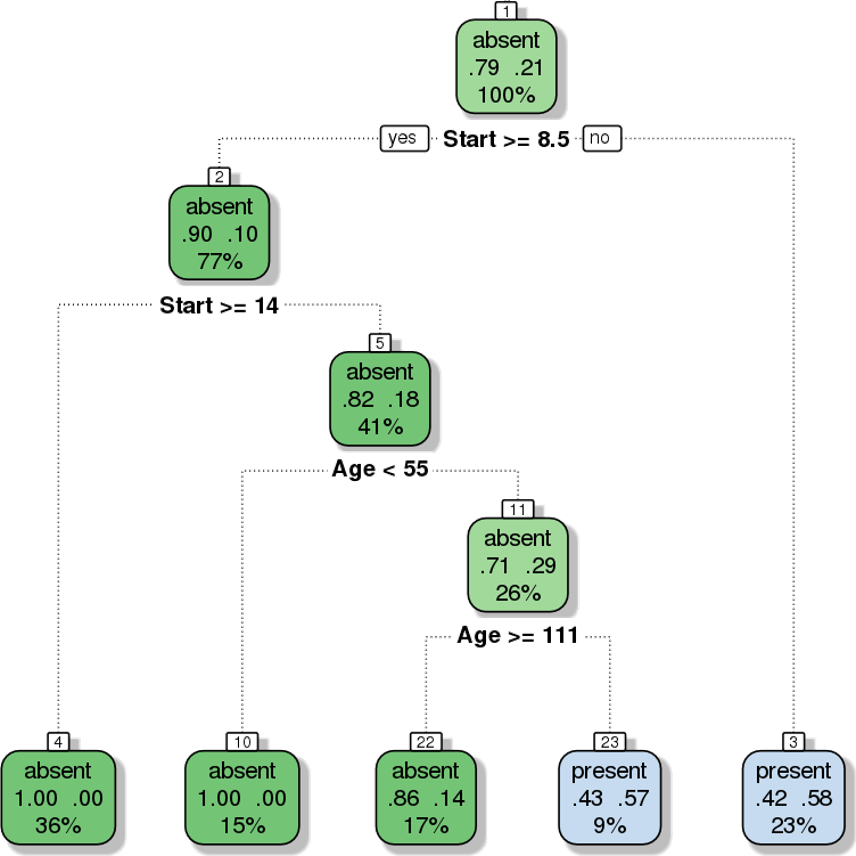
\includegraphics[width=0.25\textheight]{images/DSML/kyphosistree.png}
\caption{\small Decision tree}\label{fig:class8a}
\end{subfigure}
\begin{subfigure}[m]{0.45\textwidth}
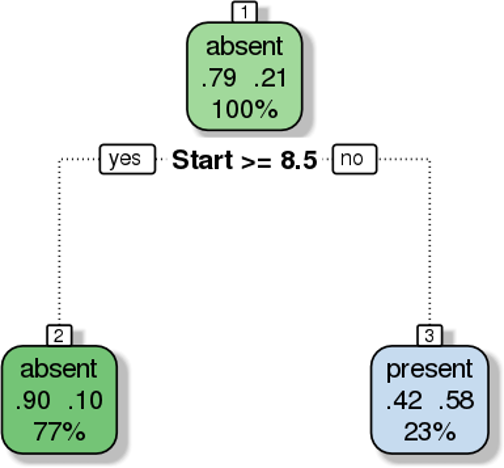
\includegraphics[width=0.25\textheight]{images/DSML/prunedkyphosistree.png}
\caption{\small Pruned decision tree}\label{fig:class8b}
\end{subfigure}
\caption[\small Pruning a decision tree]{\small Pruning a decision tree -- the original tree is more accurate, but substantially more complex than the pruned tree.}\label{fig:class8}
\end{figure}
\afterpage{\FloatBarrier}
 \begin{table}[!t]
\centering
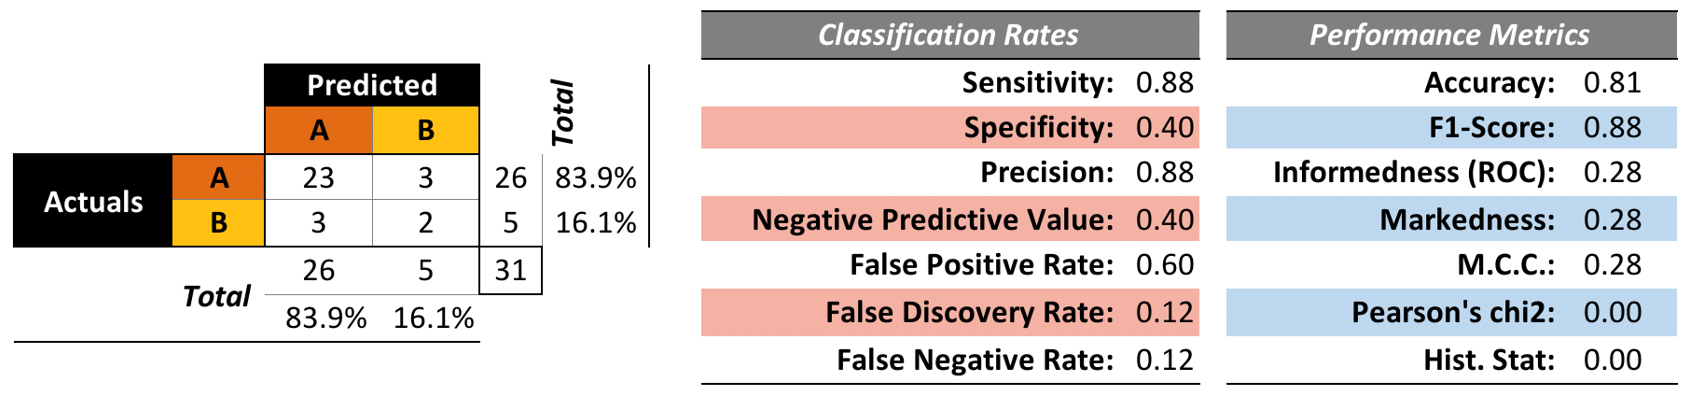
\includegraphics[width=\textwidth]{images/DSML/kyphosis4.png}
\caption[\small Kyphosis decision tree -- performance evaluation]{\small Kyphosis decision tree -- performance evaluation. The accuracy and $F1$ score are good, but the false discovery rate and false negative rate are not so great. This tree is good at predicting successful surgeries, but not fantatstic at predicting failed surgeries. Is it useful?}\hrule \label{fig:class9}
\end{table}
\afterpage{\FloatBarrier}
\subsubsection{Unsupervised Learning and Clustering}
\begin{tcolorbox}[title=A Never-Ending Story]
Clustering is in the eye of the beholder, and as such, researchers have proposed many induction principles and models whose corresponding optimisation problem can only be approximately solved by an even larger number of algorithms. \\[-0.6cm]
\begin{flushright}
-- V. Estivill-Castro, \textit{Why So Many Clustering Algorithms?}
\end{flushright}
\end{tcolorbox}
\noindent Quantitatively speaking, many statements can be made of a dataset: at the univariate level, we can compute frequency counts for the variables, identify measures of centrality (mean, mode, median) and dispersal (range, standard deviation), among others. At the multivariate level, various options are available, including $n-$way tabulations, correlation analysis, and data visualisation, for instance. 

While these might provide insights on simple data, sets for which there is a large number of variables and mixed types (categorical and numerical) might not yield to such an approach. Instead, insight might come in the form of \textbf{aggregation} or \textbf{clustering} of similar observations. A successful clustering scheme tightly joins together any number of similarity profiles (tight in this context refers to small variability within the cluster). A typical application is one found in search engines, who attempt to group similar objects in one cluster and dissimilar objects far from each other -- the listed results for the search are the nearest similar objects clustered around the search item. Implicit in this example (and in all applications) is the crucial factor of \textbf{closeness}: what does it mean for one observation to be near another one? Various \textbf{metrics} can be used, and not all of them lead to the same results. 

Clustering is a form of unsupervised learning since the cluster labels are not determined ahead of the analysis. Among its advantages is the fact that clusters can be determined even when there are no natural ways to break down a dataset into constituent parts. One the one hand, if there is no natural way to break up the data into clusters, the results may be entirely arbitrary and fail to represent any underlying reality of the dataset. On the other hand, it could turn out that there were no recognized ways to naturally break up the data into clusters, and the clustering algorithm may discover such a grouping -- clustering is sometimes called \textbf{automated classification} as a result. Figure~\ref{fig:clust2} illustrates the main notion of clustering over a an artificial dataset. \newpage\noindent
In \textbf{clustering}, the data is divided into \textbf{naturally occurring groups}. Within each group, the data points are similar; from group to group, they are dissimilar (see Figure~\ref{fig:clust1}). 
\begin{figure}[!t]
\centering
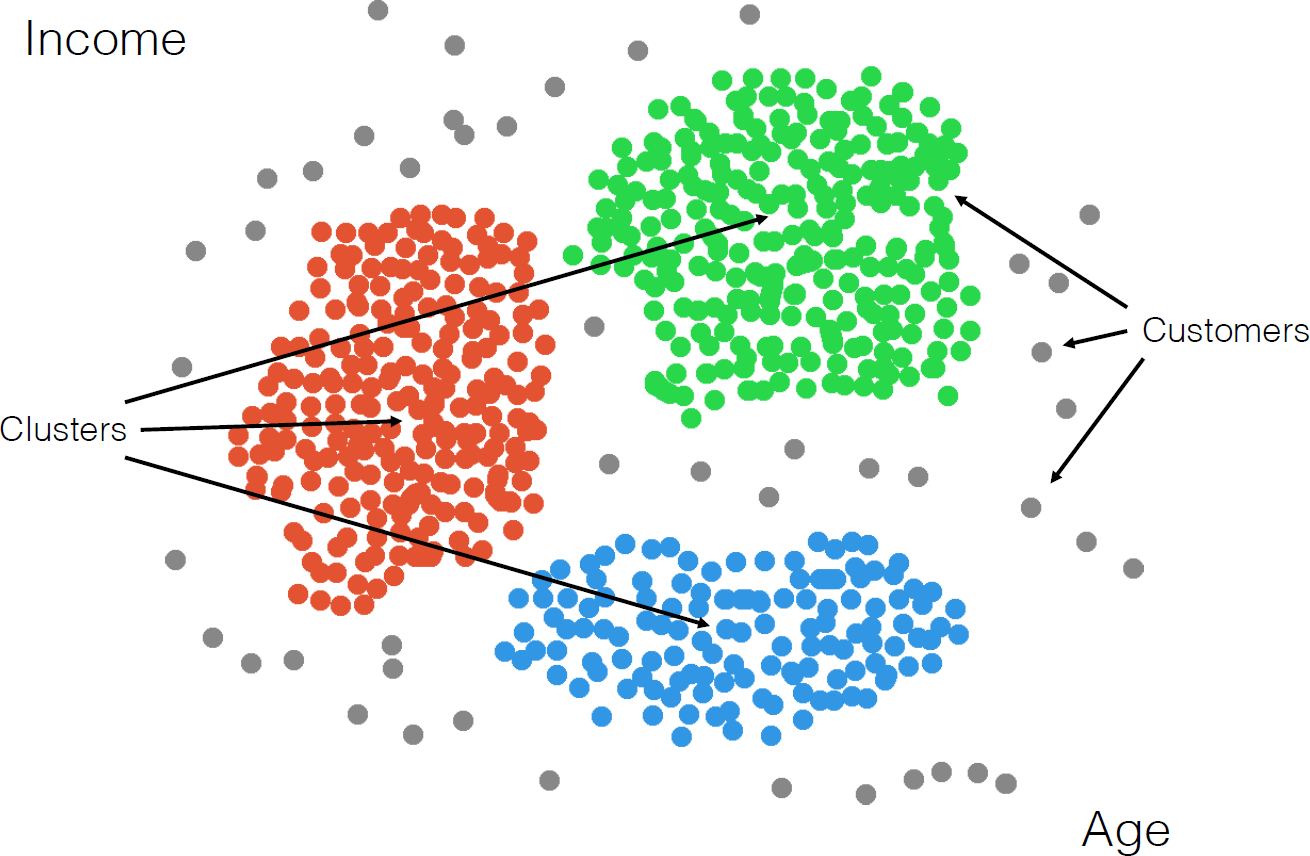
\includegraphics[width=\textwidth]{images/DSML/clustering2.png}
\caption[\small Clusters and outliers in an artificial dataset]{\small Clusters and outliers in an artificial dataset.}\label{fig:clust2}
\end{figure}
\afterpage{\FloatBarrier}
\begin{figure}[!t]
\centering
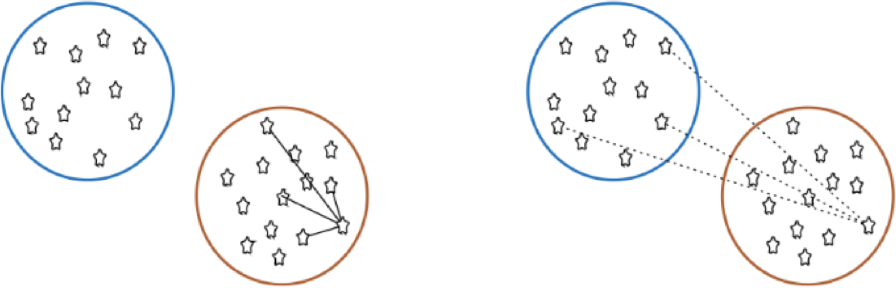
\includegraphics[width=0.75\textwidth]{images/DSML/clustering1.png}
\caption[\small Cluster distances.]{\small Average distance to points in own clusters (left, smaller is better) and to points in other clusters (right, larger is better).}\hrule\label{fig:clust1}
\end{figure}
\afterpage{\FloatBarrier}
Clustering as a learning mechanism is relatively \textbf{intuitive} for human beings as our brains unconsciously search for patterns. In general, people can handle \textbf{messy} data with the same relative ease as they handle clean data, but computers have a harder time doing so -- part of the difficulty is that there is no \textbf{agreed-upon definition of what constitutes a cluster}, and so we cannot easily code their recognition into algorithms. To paraphrase Justice Potter Stewart, 
\begin{quote}I may not be able to define what a cluster is, but I know one when I see one.
\end{quote}
\newpage\noindent Clustering algorithms can be \textbf{complex} and \textbf{non-intuitive}, based on varying notions of similarities between observations, and yet,  the temptation to provide a simple \textit{a posteriori} explanation for clustering results remains \textbf{strong} -- we really, really want to reason with the data. Were you able to look at Figure~\ref{fig:clust2} without assigning labels or trying to understand what type of customers were likely to be young and have medium incume? older and wealthier?  Clustering algorithms are also (typically) \textbf{non-deterministic} -- the same routine, applied twice (or more) to the same dataset, can discover completely different clusters (the order in which the data is presented can play a role, so can starting configurations)! 
\newl
\textbf{IMPORTANT NOTE:} this (potential) non-replicability is not just problematic for validation, it can also leads to client dissatisfaction. If the consultant is tasked with finding customer clusters for marketing purposes and the clusters change every time the client asks for a report, there will be a very confused client unless you have explained the stochastic nature of the clusters before hand. 
\begin{center}
    \rule{0.5\textwidth}{.4pt}
\end{center}
All clustering algorithms rely on the notion of \textbf{similarity} $w$ between observations; in many instances, similarity is obtained \textit{via} a \textbf{distance} (or metric) $d$. Typically, $w\to 1$ as $d\to 0$ and $w\to 0$ as $d\to\infty$, but there are similarity measures which are not derived from a distance metric. One additional source of clustering challenge is that there is no such thing as \textbf{the} distance  or \textbf{the} similarity measure between observations, and that observations which are similar using a specific measure may not be similar at all using another. Commonly-used metrics include: Euclidean, Manhattan, Cosine, Canberra, Haming, Jaccard, Pearson, and so forth (see Figure~\ref{fig:clust3}). In general, however, no matter which similarity measure is selected, the data must first be \textbf{transformed} (scaled, centered, etc.), which introduces another layer of difficulty as there is not a canonical way to do this. 
\begin{figure}[!t]
\centering
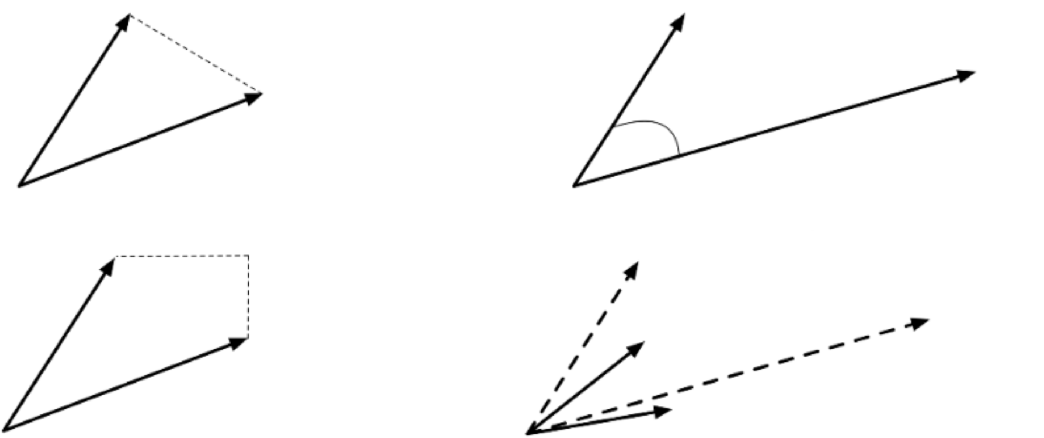
\includegraphics[width=\textwidth]{images/DSML/clustering3.png}
\caption[\small Distance metrics between observations.]{\small Distance metrics between observations: Euclidean (as the crow flies, top left); cosine (direction from a vantage point, top right); Manhattan (taxi-cab, bottom left). Observations should be transformed (scaled, translated) before distance computations (bottom right).)}\hrule\label{fig:clust3}
\end{figure}
\afterpage{\FloatBarrier}
\newpage\noindent
Clustering and other unsupervised learning tasks are frequently used, but often as preliminary steps in supervised learning problems -- there are stand-alone applications as well: 
\begin{itemize}[noitemsep]
\item \textbf{text analysis} -- grouping similar documents according to their topics, based on the patterns of common and unusual terms;
\item \textbf{product recommendations} -- grouping online purchasers based on the products they have viewed, purchased, liked, or disliked, or grouping products based on customer reviews;
\item \textbf{marketing} -- grouping client profiles based on their demographics and preferences;
\item \textbf{social network analysis} -- recognising communities within large groups of people;
\item \textbf{medical imaging} -- differentiating between different tissue types in a 3D voxel;
\item \textbf{genetics} -- inferring structures in populations;
\item dividing a larger group (or area, or category) into smaller groups, with members of the smaller groups having similarities of some kind, as analytical tasks may then be solved separately for each of the smaller groups, which may lead to increased accuracy once the separate results are aggregated, or 
\item creating (new) taxonomies on the fly, as new items are added to a group of items, which could allow for easier product navigation on a website like Netflix, for instance.
\end{itemize}
Other examples may be found in \cite{DSML_CL1,DSML_CL5,DSML_CL6,DSML_CL7,DSML_CL8,DSML_CL9,DSML_CL10,DSML_CL101,DSML_CL11,DSML_CL12,DSML_CL13,DSML_CL14,DSML_CL15}. 
\begin{center}
    \rule{0.5\textwidth}{.4pt}
\end{center} 
The clustering process is often the same, notwithstanding the choice of scaling strategy, similarity measure, and algorithm and parameters (see the pipeline shown in Figure~\ref{fig:clust4}). 
\begin{figure}[!t]
\centering
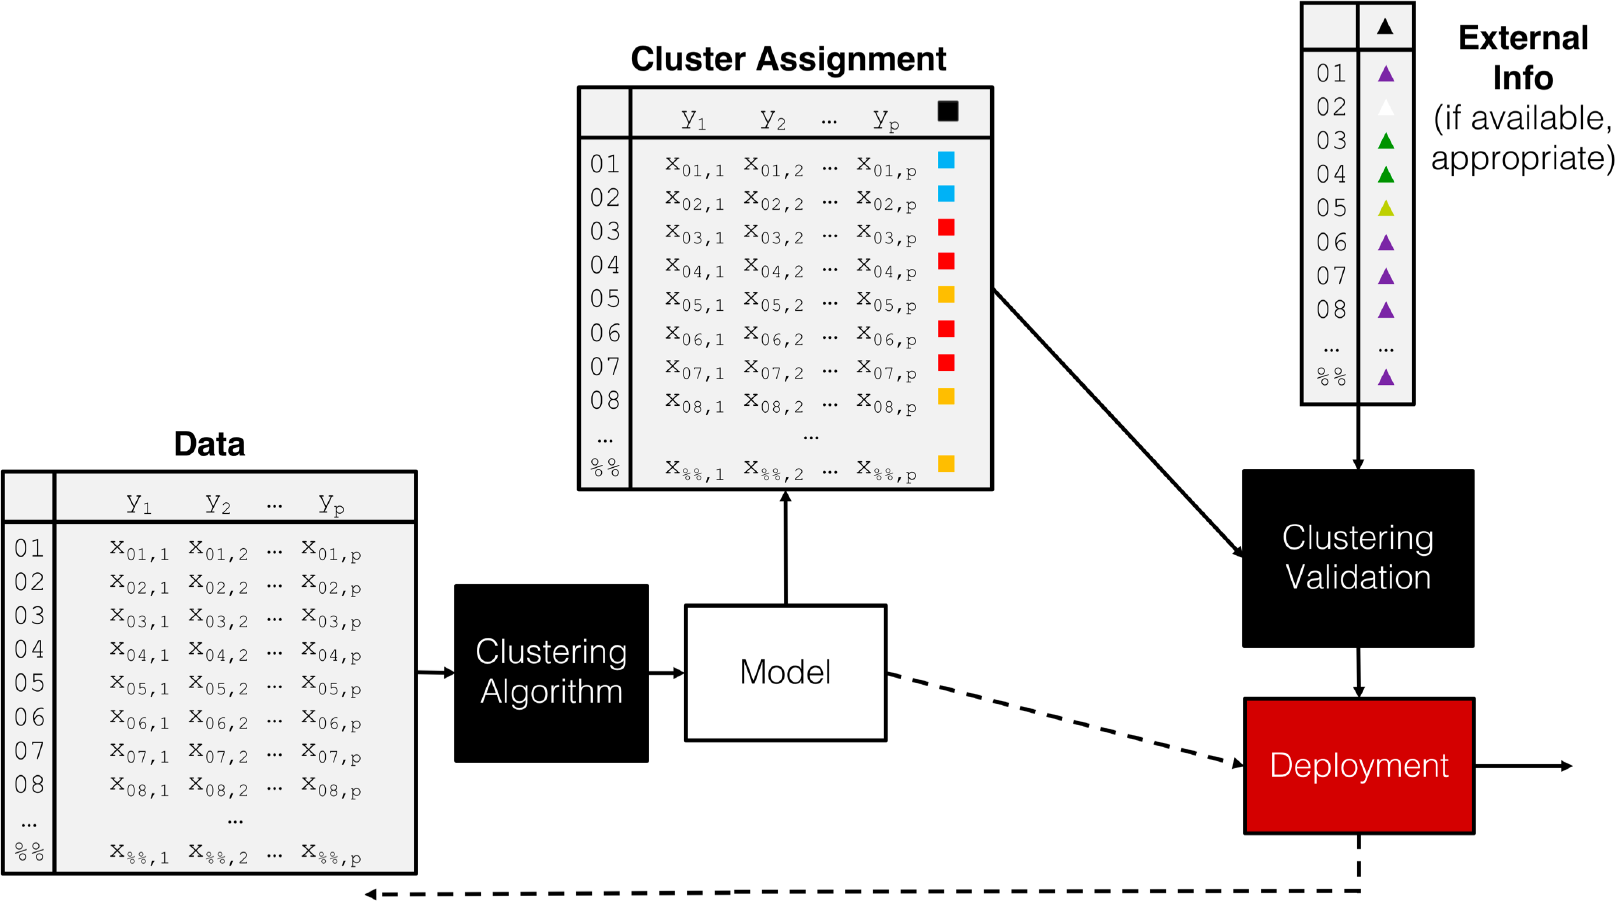
\includegraphics[width=\textwidth]{images/DSML/Clustering_Pipeline.png}
\caption[\small Clustering pipeline]{\small A clustering pipeline, including validation and (eventual) deployment}\hrule\label{fig:clust4}
\end{figure}
\afterpage{\FloatBarrier}
\begin{figure}[H]
\centering
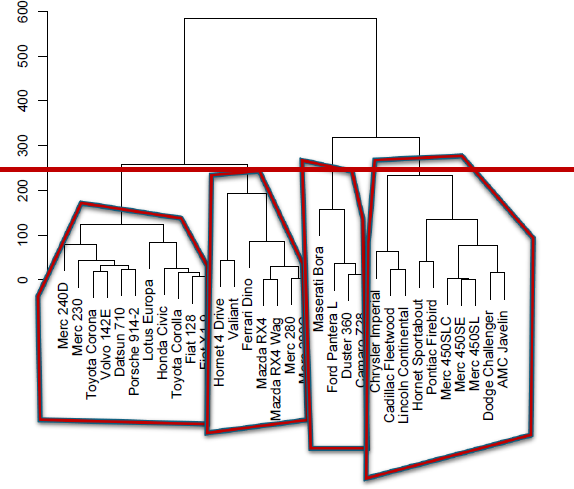
\includegraphics[width=0.3\textwidth]{images/DSML/cluster_dendrogram.png}\quad 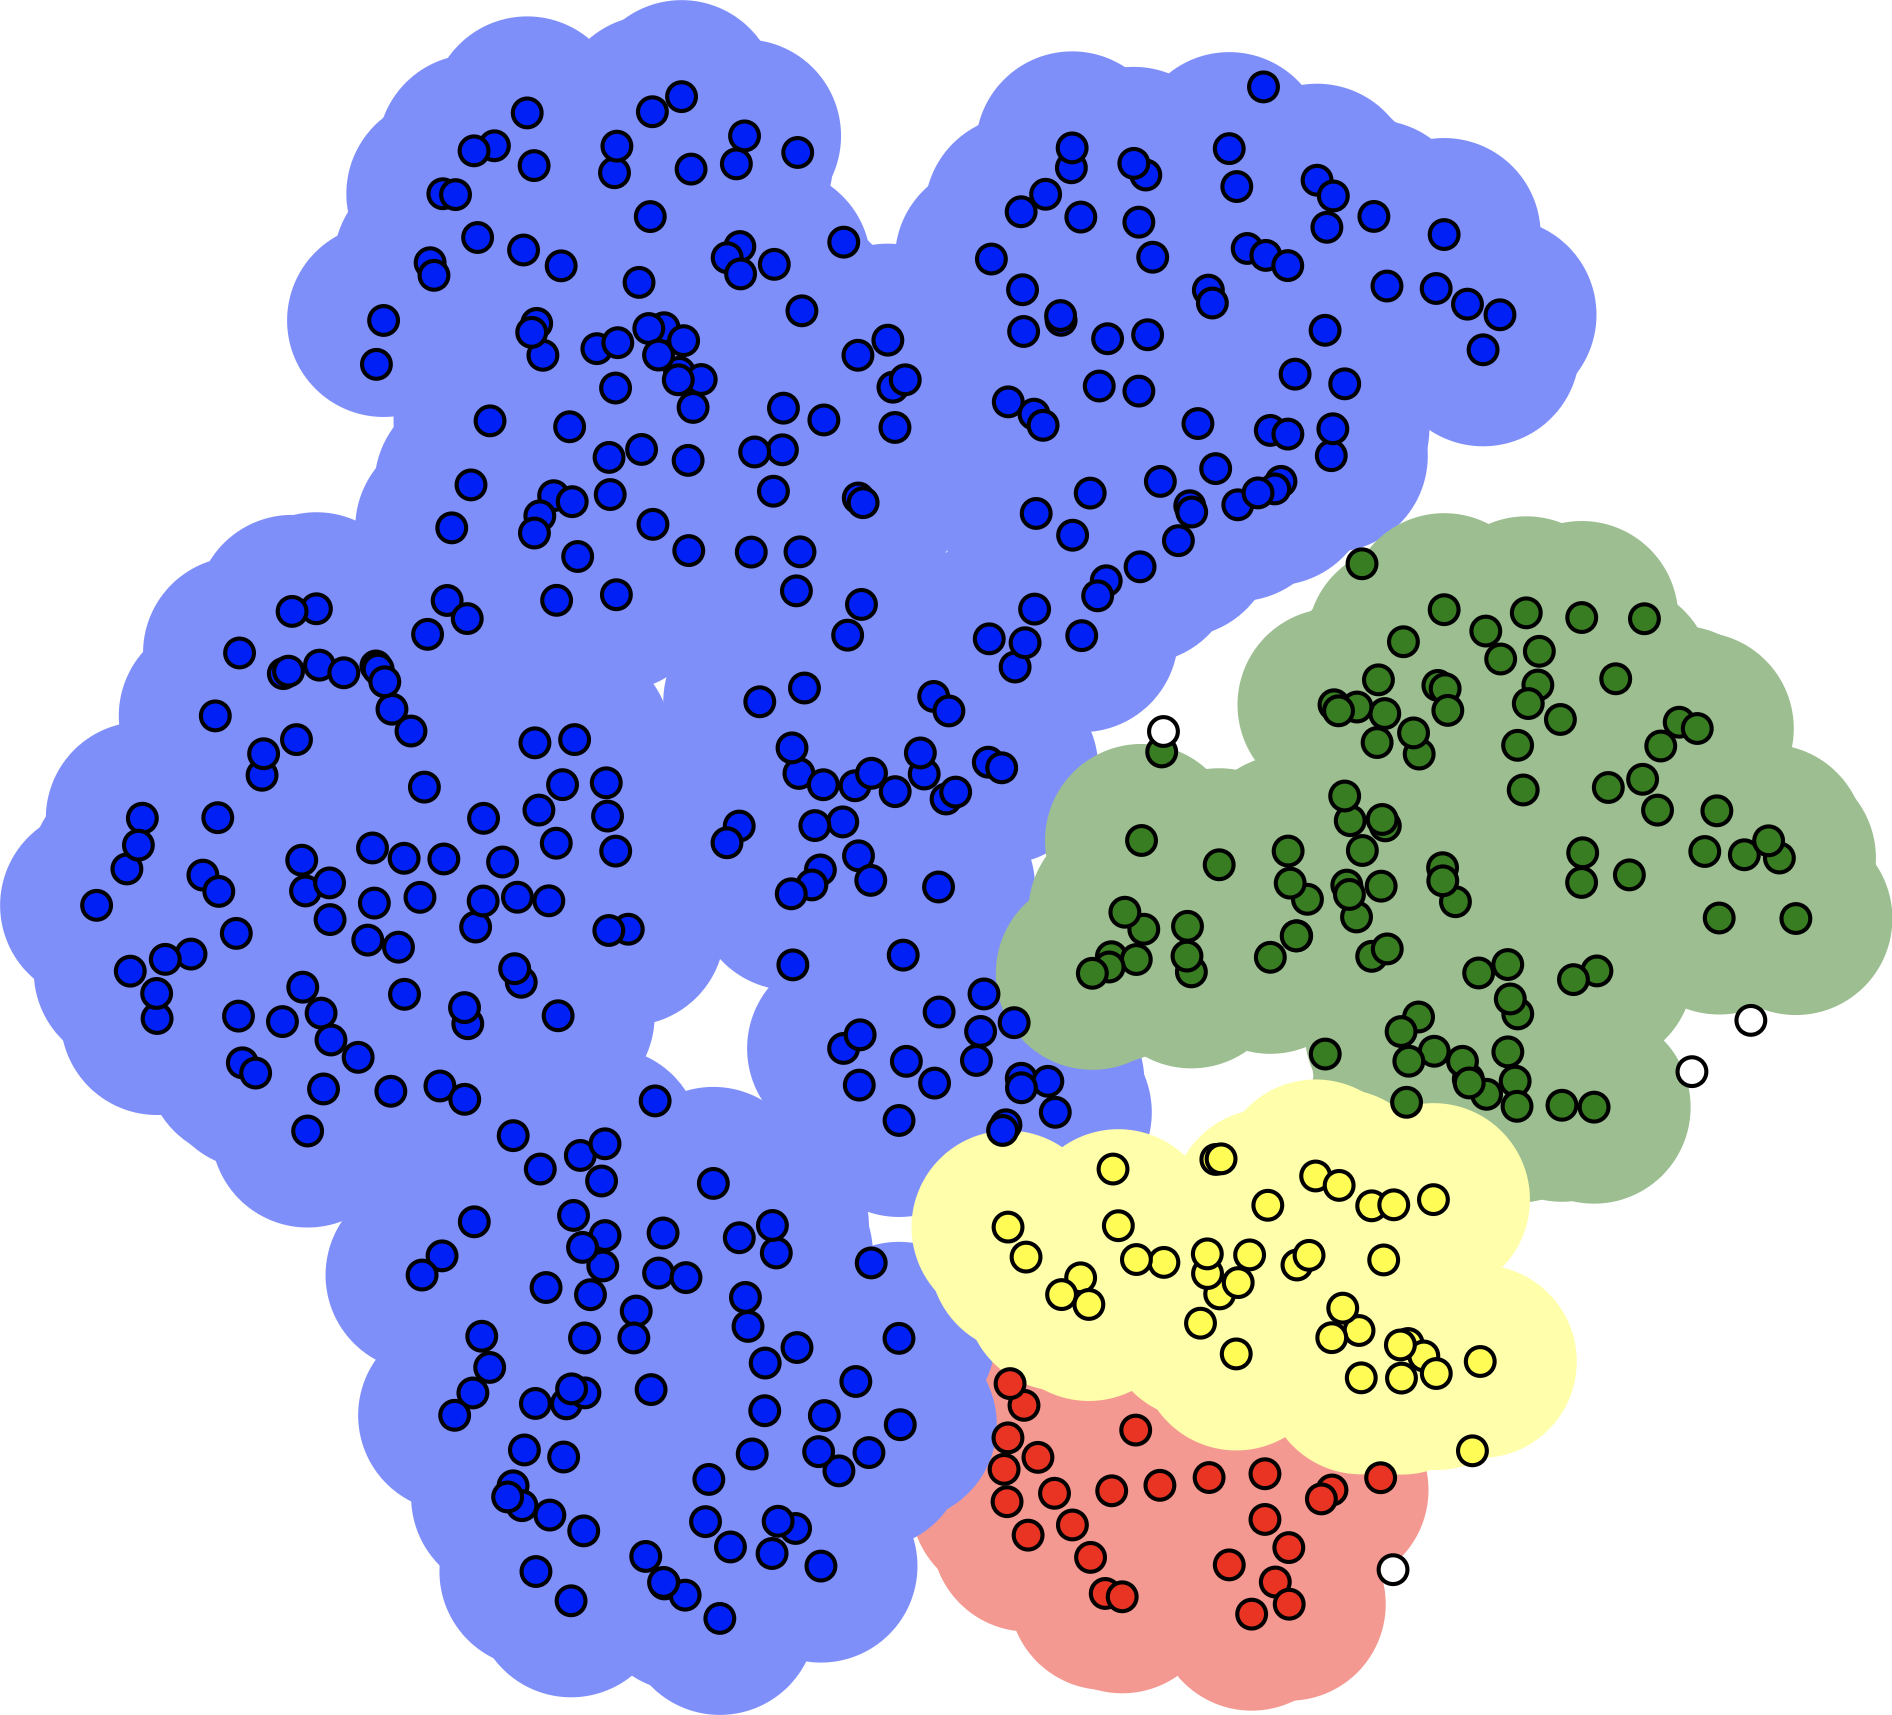
\includegraphics[width=0.3\textwidth]{images/DSML/dbscan.png}\quad 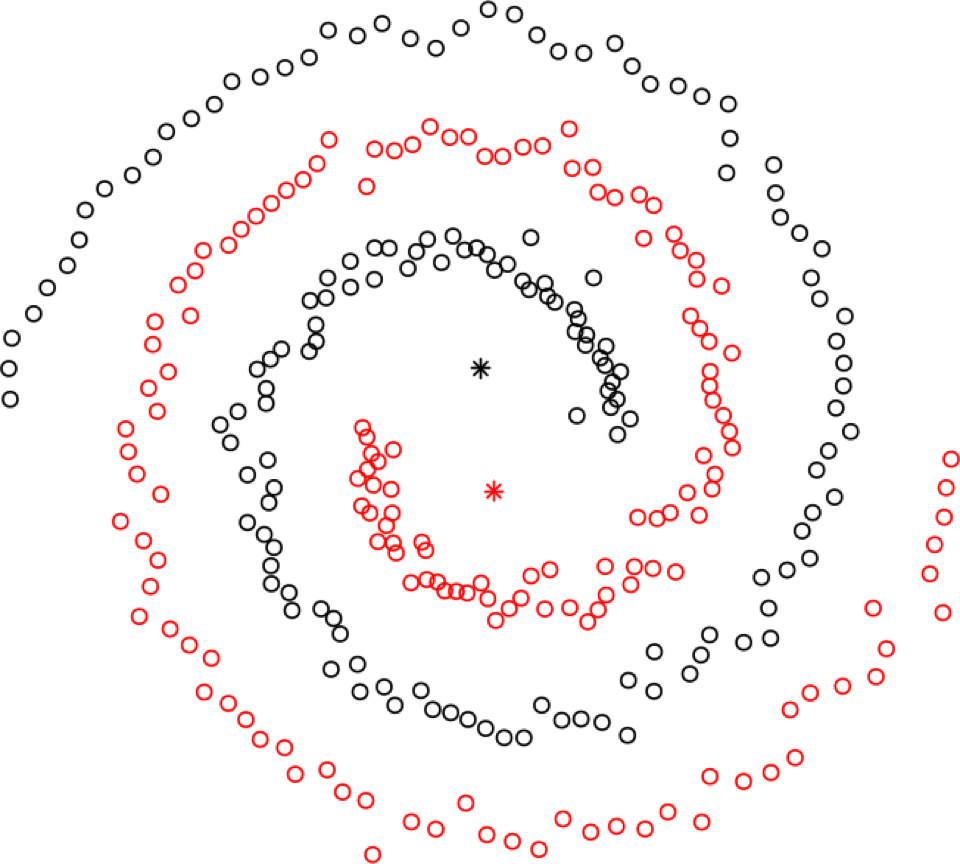
\includegraphics[width=0.3\textwidth]{images/DSML/spectral.png}
\caption[\small Illustration of hierarchical clustering, DBSCAN, and spectral clustering]{\small Illustration of hierarchical clustering (left), DBSCAN (middle, based on \cite{DSML_CL20}), and spectral clustering (right).}\hrule\label{fig:clustden}
\end{figure}
\afterpage{\FloatBarrier}
\paragraph{Clustering Algorithms} As is the case with classification, the number of clustering algorithms is quite high; the Wikipedia page lists 40+ such algorithms as of August 2018 \cite{DSML_CL16}. The choice of algorithms (and associated parameters) is as much an art as it is a science, although domain expertise can come in handy \cite{DSML_CL1}. Here are common algorithms that data scientists should have at their command (full descriptions available in \cite{DSML_T,DSML_PF,DSML_CL1}):
\begin{itemize}[noitemsep]
\item \textbf{$k-$means}, close on the heels of decision trees for the title of ``most-used data science algorithm'', is a partition clustering method, which tends to produce equal-sized clusters; when clients ask for their data to be clustered, they typically envision $k-$means with the Euclidean metric; variants exists such as $k-$mode (for categorical data), $k-$medians (for data with outliers), $k-$means$||$ and $k-$means$++$ for large data sets; the number of clusters $k$ (and the similarity measure/distance metric) must be provided by the user; works fairly well for ``blob''-like data; 
\item \textbf{hierarchical clustering} is one of the few deterministic algorithms on the market; there are divisive (DIANA) and agglomerative (AGNES) versions; there are no parameters to input, but the users must select a \textbf{linkage} strategy (roughly speaking, a metric that computes the distance between clusters) and a level at which to read off the clusters (see Figure~\ref{fig:clustden});  
\item \textbf{density-based spatial clustering} which is typically graph-based and attempts to identify closely-packed regions of the dataset; obvious advantages of DBSCAN (and variants OPTICS and DENCLUE) is robustness to outliers and not needing to be told how many clusters to search in the data; the main disadvantage is that the input parameters (neighbourhood radius and minimum number of points to be considered dense) are not easy to derive;  
\item \textbf{affinity propagation} is another clustering algorithm which selectes the optimal number of clusters directly from the data, but it does so by trying out and evaluating various scenarios and evaluating which may end up being time-consuming; 
\item \textbf{spectral clustering} can be used to recognise non-globular clusters; these are found by computing eigenvalues of an associated laplacian matrix -- consequently, spectral clustering is fast. 
\end{itemize}
Other methods include \textbf{latent Dirichlet allocation} (which is used in topics modeling), \textbf{expectation-maximisation} (particularly useful to find gaussian clusters), \textbf{BIRCH} (a local method which does not require the entire dataset to be scanned) and \textbf{fuzzy clustering} (a soft clustering scheme in which the observations have a degree of belonging to each cluster). 
\begin{figure}[!t]
\centering
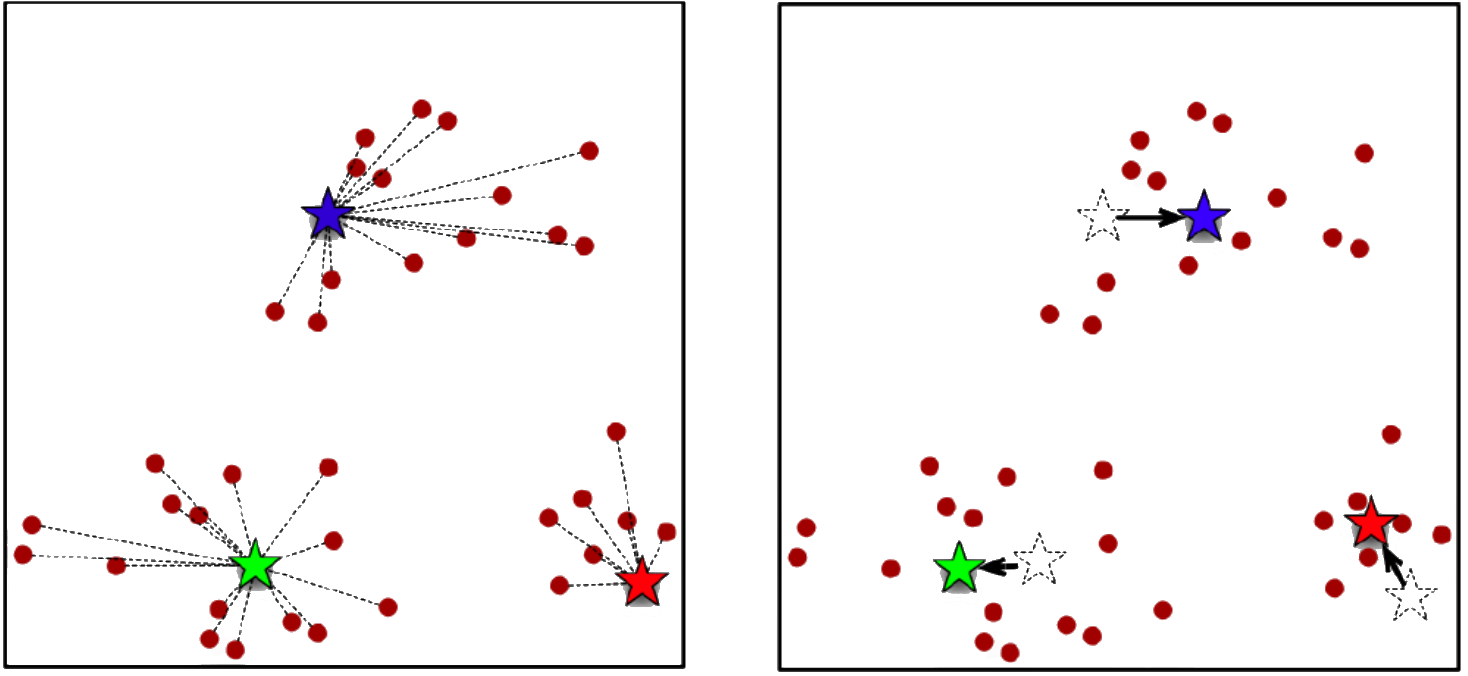
\includegraphics[width=\textwidth]{images/DSML/clustering5.png}
\caption[\small $k-$means cluster allocation and updated centres.]{\small $k-$means cluster allocation (left) and updated centres (right).}\hrule\label{fig:clust5}
\end{figure}
\afterpage{\FloatBarrier}
\paragraph{$k-$ Means} As mentioned previously, $k-$means is a very natural way to group observations together (formally, $k-$means is linked to \textbf{Voronoi tilings}): clustering is achieved by 
\begin{enumerate}[noitemsep]
\item selecting a \textbf{distance metric} $d$ (based on the data type and domain expertise);
\item selecting a \textbf{number of clusters} $k$;
\item randomly choosing $k$ data instances as initial \textbf{cluster centres};
\item calculating the \textbf{distance} from each observation to each centre;
\item placing each instance in the cluster whose centre it is \textbf{nearest} to;
\item computing/updating the \textbf{centroid} for each cluster (see Figure~\ref{fig:clust5});
\item repeating steps 4-6 until the clusters are \textbf{stable}.
\end{enumerate}
For $k-$means, cluster centroids is obtained by averaging all points in the cluster. For $k-$medians and $k-$mode, the centrality measure is replaced by the obvious candidate. \newl 
This simple algorithm has numerous strengths: 
\begin{itemize}[noitemsep]
\item it is elegant and \textbf{easy to implement} (without actually having to compute pairwise distances), and so is extremely common as a result;
\item in many contexts, it is a \textbf{natural way} to look at grouping observations, and 
\item it helps provide a first-pass \textbf{basic understanding of the data structure}. 
\end{itemize}
On the other hand,
\begin{itemize}[noitemsep]
\item it can only assign an instance to \textbf{one} cluster, which can lead to overfitting -- a more robust solution would be to compute the probability of belonging to each cluster, perhaps based on the distance to the centroid; 
\item it requires the ``true'' underlying clusters to be \textbf{gaussian-} or blob-shaped, and it will fail to to produce useful clusters if that assumption is not met in practice, 
\item it does not allow for \textbf{overlapping} or \textbf{hierarchical} groupings. 
\end{itemize}
\newpage\noindent Let \begin{figure}[!t]
\centering
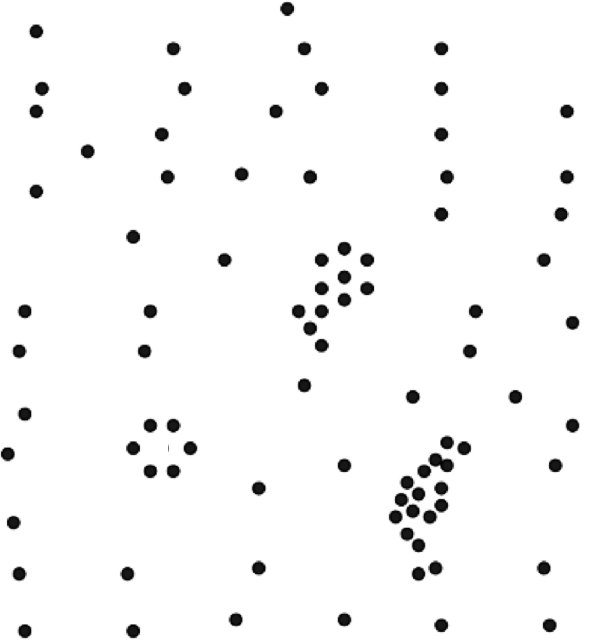
\includegraphics[width=0.20\textwidth]{images/DSML/clustering6.png} \qquad\qquad 
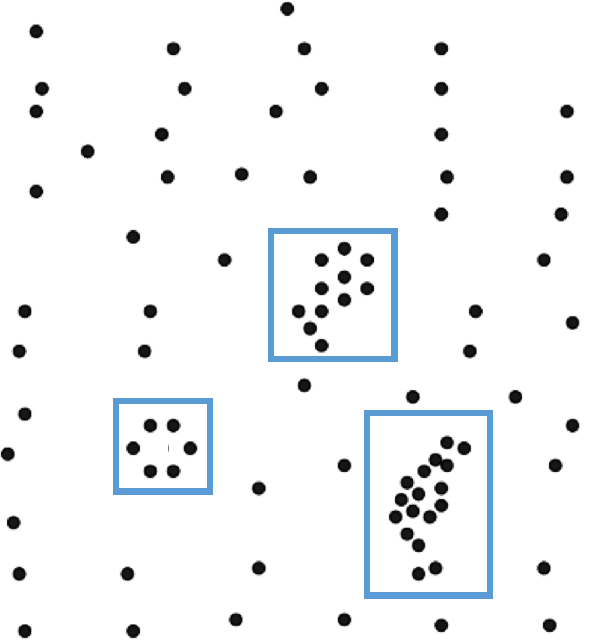
\includegraphics[width=0.2\textwidth]{images/DSML/clustering7.png} \qquad\qquad
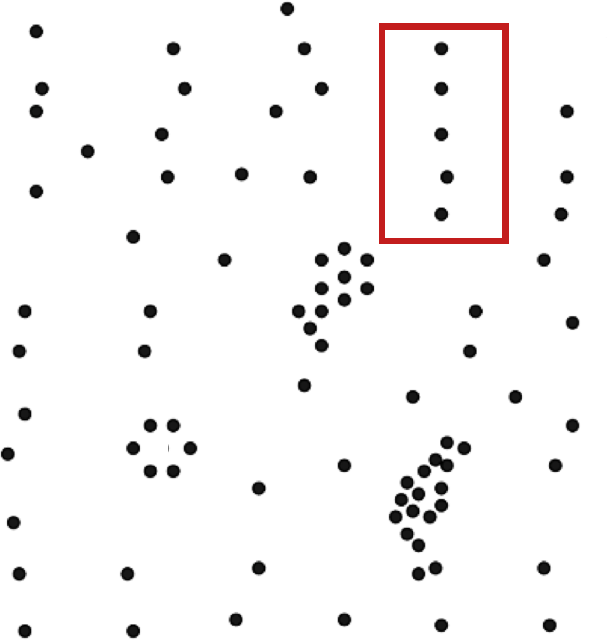
\includegraphics[width=0.2\textwidth]{images/DSML/clustering8.png} \caption[\small Cluster suggestions in an artificial dataset]{\small Artificial dataset; suggested clusters (blue), rejected suggestion (red).}\hrule\label{fig:clust678}
\end{figure}
\afterpage{\FloatBarrier}
 us dwell some more on some of the issues relating to clustering \textbf{in general} (as opposed to specific to $k-$means):
\begin{itemize}[noitemsep]
\item an implicit gamble is made, that of nearness of observations (in some metric) being linked with similarity, and large distances with dissimilarity -- there are plenty of situations where this is an appropriate assumption to make (temperature readings on a map, for instance), but also many situations where it is less likely to be the case (physical proximity at a grocery's checkout counter, say... it is harder to find an example in this case due to our pattern-seeking habits, but the point remains solid);  
\item the \textbf{lack of a clear-cut definition} of what a cluster actually is makes it difficult to validate clustering results, although some guidelines exist (see Figure~\ref{fig:clust678});
\item the fact that various algorithms are \textbf{non-deterministic} is also problematic, and suggests that a clustering scheme should never be obtained using only one algorithmic pass; the outcome could be different depending on the \textbf{location} of random starting positions and the distance/similarity metric in use; essential patterns may emerge if the algorithms are implemented multiple times, with different starting positions and re-ordered data -- for more information on the topic, see \textbf{cluster ensembles} in \cite{DSML_CL1};
\item for those algorithms that require the \textbf{number of clusters} as an input, it is difficult to determine what the optimal number should be (see Figure~\ref{fig:clust9}); this number obviously depends on the choice of algorithm/metric, the underlying data, and the use that will be made of the resulting clusters -- a dataset could have 3 natural groups when seen through the lens of $k-$means, but only 2 for a specific choice of parameter values in DBSCAN, say; a potential solution is to produce clustering schemes (from the same family of algorithms) with an increasing number of clusters and to plot the average distance of a cluster member to its cluster representative (centroid) against the number of clusters, and to look for ``kinks'' in the plot -- such points provide cluster numbers at which an increase does not provide an in-step increase in clustering ``resolution'', so to speak; 
\item even when a cluster scheme has been accepted as valid, a \textbf{cluster description} might be difficult to come by -- recall the examples provided when describing natural groups for unsupervised learning on \pageref{unsl} -- should clusters be described using representative instances or average values or some combination of its' members most salient features?;
\item most methods will find clusters in the data even if there are none -- although DBSCAN is exempt from this \textbf{ghost clustering} (see Figure~\ref{fig:clust1011}), and 
\item beware the temptation of \textbf{\textit{a postiori} rationalisation} -- once clusters have been found, it is tempting to try to ``explain'' them, but that is a job for domain experts, at best, and a waste of time and resources, at worst. 
\end{itemize}
\begin{figure}[!t]
\centering
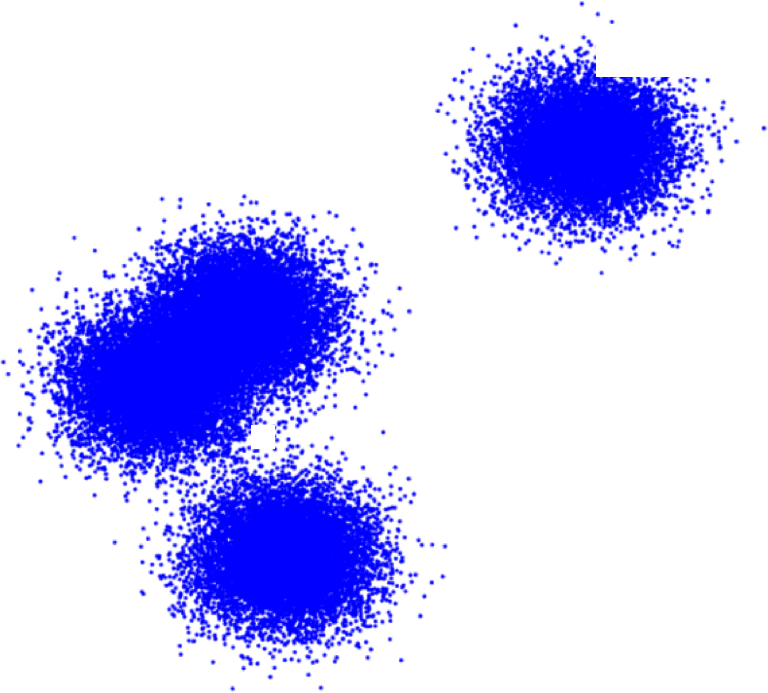
\includegraphics[width=0.5\textwidth]{images/DSML/clustering9.png}  \caption[\small Ambiguous number of clusters]{\small The number of clusters in a dataset is ambiguous: are there 2, 3, 4 or more clusters here?}\label{fig:clust9}
\end{figure}
\afterpage{\FloatBarrier}
\begin{figure}[!t]
\centering
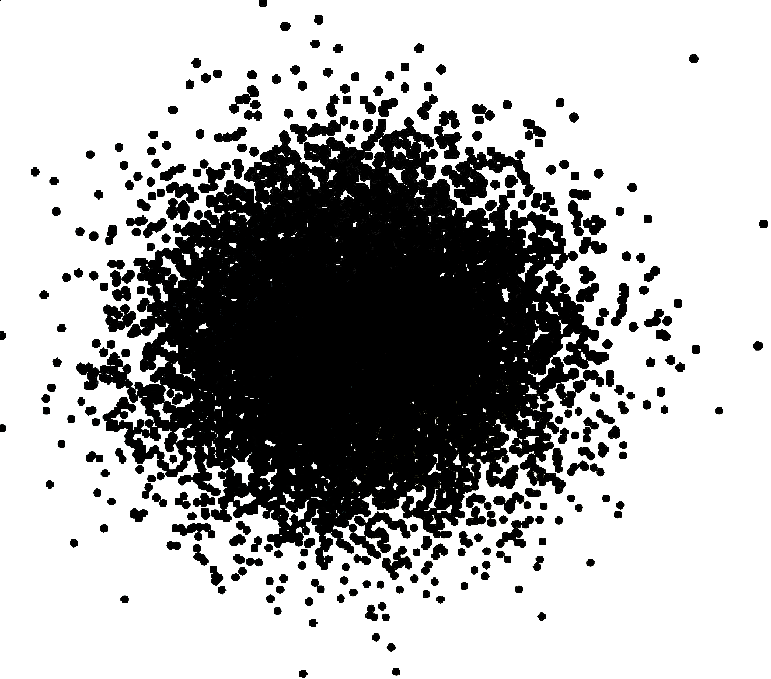
\includegraphics[width=0.45\textwidth]{images/DSML/clustering10.png}\quad 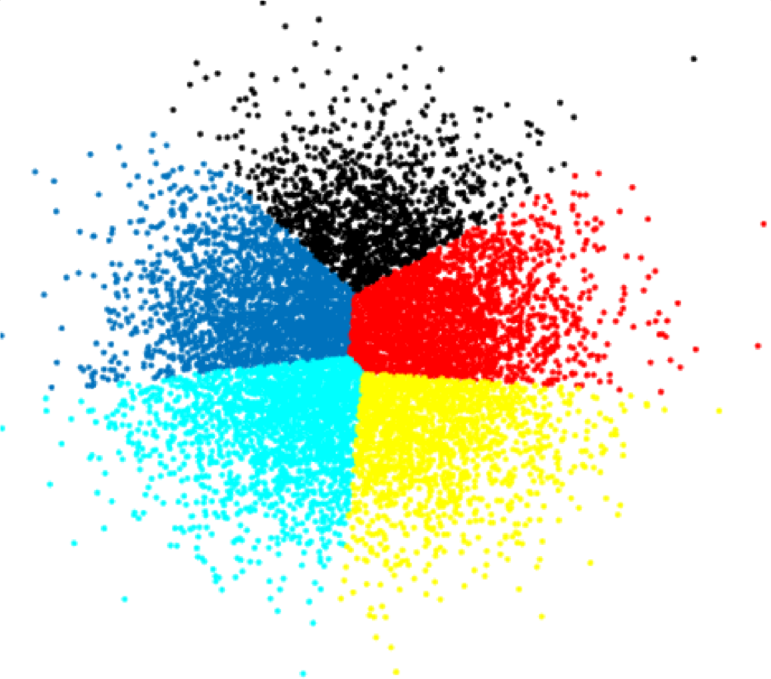
\includegraphics[width=0.45\textwidth]{images/DSML/clustering11.png}  \caption[\small An illustration of ghost clustering with $k-$means]{\small An illustration of ghost clustering with $k-$means, for $k=5$.}\hrule\label{fig:clust1011}
\end{figure}
\afterpage{\FloatBarrier}
\paragraph{Clustering Validation} 
What does it mean for a clustering scheme to be \textbf{better} than another? What does it mean for a clustering scheme to be \textbf{valid}? What does it mean for a single cluster to be \textbf{good}? \textbf{How many} clusters are there in the data, really? These are not easy questions to answer. In general, asking if a clustering scheme is the right one or a good one is meaningless -- much better to ask if it is \textbf{optimal} or \textbf{sub-optimal}.\newl 
An \textbf{optimal} clustering scheme is one which 
\begin{itemize}[noitemsep]
\item maximises separation between clusters;
\item maximises similarity within groups;
\item agrees with a human eye test, and 
\item is useful at achieving its goals.
\end{itemize}
There are three main families of \textbf{clustering validation}:
\begin{itemize}[noitemsep]
\item external, which uses additional information (but the labels in question might have very little to do with the similarity of the observations);
\item internal, which uses only the clustering results (shape and size of clusters, etc), and
\item relative, which compares across a number of clustering attempts.
\end{itemize}
Consider a clustering scheme $\mathcal{C}=\{\mathcal{C}_1,\ldots,\mathcal{C}_N\}$, with $\mathcal{C}_m$'s centroid denoted by $c_m$, and the average distance of $\mathcal{C}_m$'s members to $c_m$ denoted by $s_m$.  
The \textbf{Davies-Bouldin Index} is defined as $$\textrm{DB}_{\mathcal{C}}=\frac{1}{N}=\sum_{i=1}^N \max_{j\neq i}\left\{\frac{s_i+s_j}{d(c_i,c_j)}\right\},$$ where $d$ is the appropriate distance metric. Since $\textrm{DB}_{\mathcal{C}}$ is only defined using the clustering results, it is an internal validation method. Heuristically, if the clusters are not greatly separated, we might expect $d(c_i,c_j)$ to be (relatively) small, and so $\textrm{DB}_{\mathcal{C}}$ to be (relatively) large. In the same vein, if the clusters are not homogeneous, we might expect $s_i+s_j$ to be (relatively) large, and so $\textrm{DB}_{\mathcal{C}}$ to be (relatively) large. In short, when the clustering scheme is not optimal, $\textrm{DB}_{\mathcal{C}}$ should be ``large''. This suggests another way to determine the optimal number of clusters -- simply attempt to minimise $\textrm{DB}_{\mathcal{C}}$. Other methods have been suggested, let us briefly mention the \textbf{Sum of Squared Errors}, \textbf{Dunn's Index} and the \textbf{Silhouette Metric}. 
\begin{center}
    \rule{0.5\textwidth}{.4pt}
\end{center} 
\begin{figure}[!t]
\centering
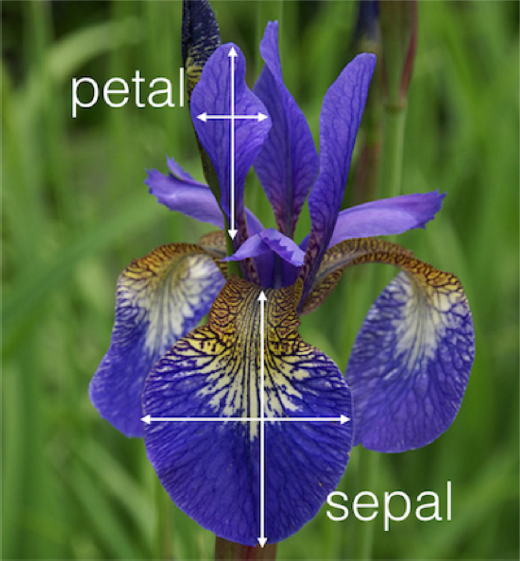
\includegraphics[height=0.3\textheight]{images/DSML/clustering12.png}\quad 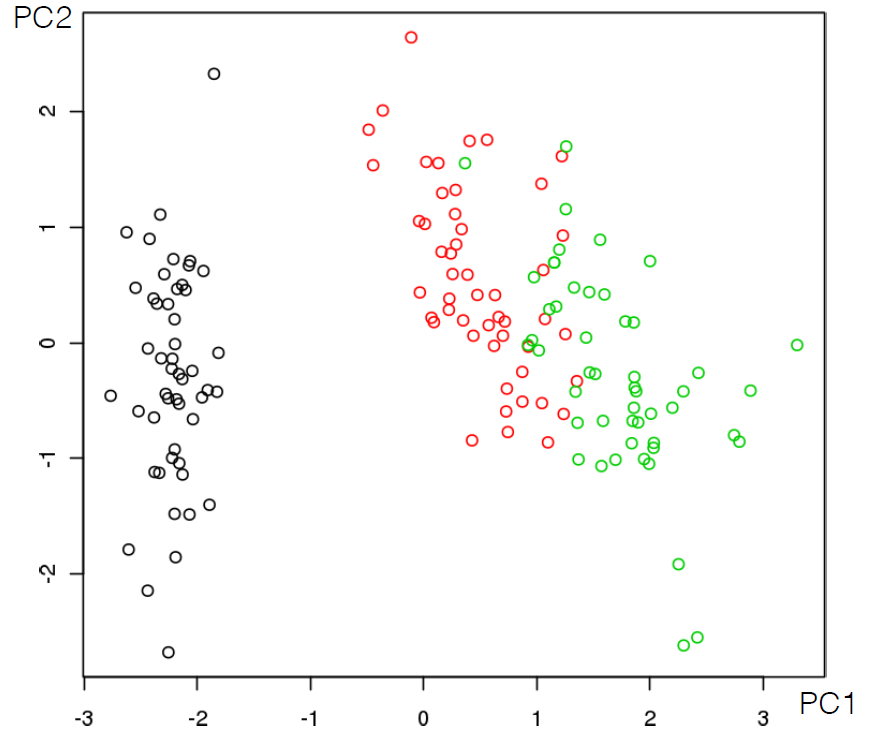
\includegraphics[height=0.3\textheight]{images/DSML/clustering13.png} 
\caption[\small Illustration of iris measurements and dataset visualisation.]{\small Illustration of iris measurements (left) and classification along 3 species, projected on 2 first principal components.}\hrule\label{fig:clust1213}
\end{figure}
\afterpage{\FloatBarrier}
Iris is a genus of plants with showy flowers. Fisher's iris dataset contains 150 observations of 5 attributes for specimens collected by Anderson, mostly from a Gasp\'e peninsula's pasture in the 1930s \cite{DSML_CL21}. The attributes are \textbf{petal width}, \textbf{petal length}, \textbf{sepal width}, \textbf{sepal length}, and \textbf{species} (virginica, versicolor, setosa). A ``description'' of these features is provided by the picture in Figure~\ref{fig:clust1213} (left). This dataset has become synonymous with data analysis (to the point that the standard joke is that ``it's not necessary to be a gardener to become a data analyst, but it helps''), being used to showcase just about every algorithm under the sun. This is, sadly, also what we are going to do. \newl A principal component projection of the dataset, with species indicated by colours, is shown in Figure~\ref{fig:clust1213} (right). From an unsupervised learning point of view, one question of interest is whether the observations form natural groupings, and, if so, whether these groupings correspond to the (known) species. \newl We use the $k-$means algorithm with Euclidean distance to resolve the problem. Since we do not know how many clusters there should be in the data (the fact that there are 3 species does not mean that there should be 3 clusters), we run 40 replicates for $k=2, \ldots, 15$ and compute a (modified) Davies-Bouldin index and Sums of Squared Errors for each of the clustering schemes. The results for a single replicate are shown for $k=2,3,4,15$ in Figure~\ref{fig:clust14151617}; validation indicates that there seems to be either $3$ of $5$ natural $k-$means clusters in the data (see Figure~\ref{fig:clust1819}). A single replicate with $k=5$ is shown in Figure~\ref{fig:clust20}. Is it surprising that $k=3$ was one of the candidates? Would you consider the final clustering scheme to be meaningful? 
\begin{figure}[t]
\centering
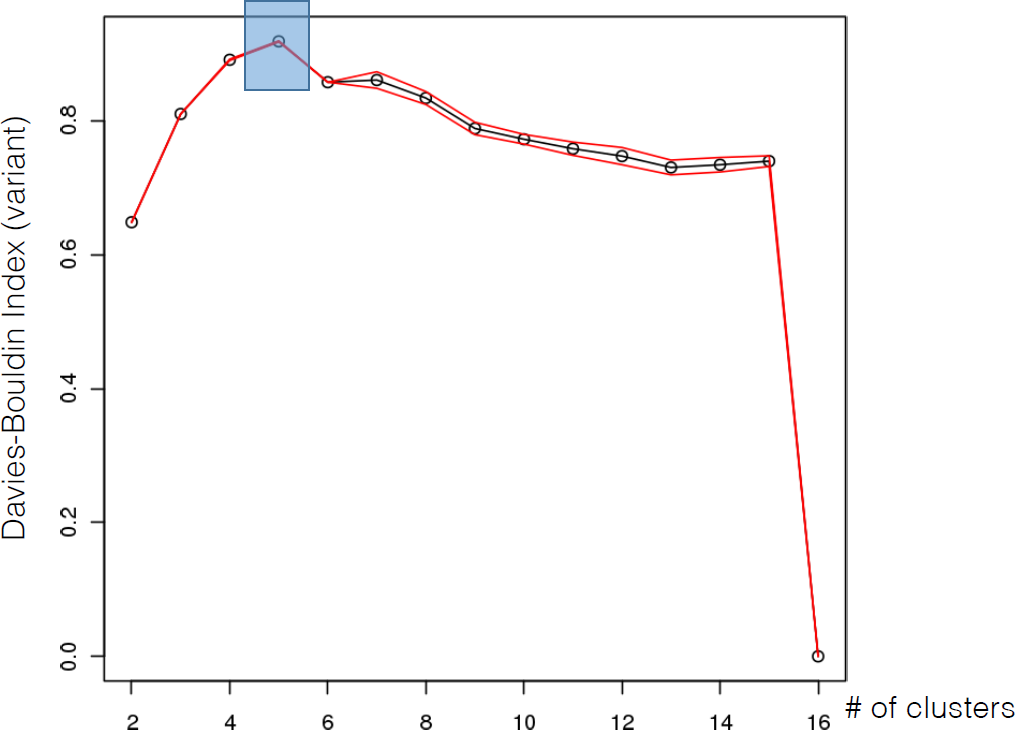
\includegraphics[width=0.40\textwidth]{images/DSML/clustering18.png}
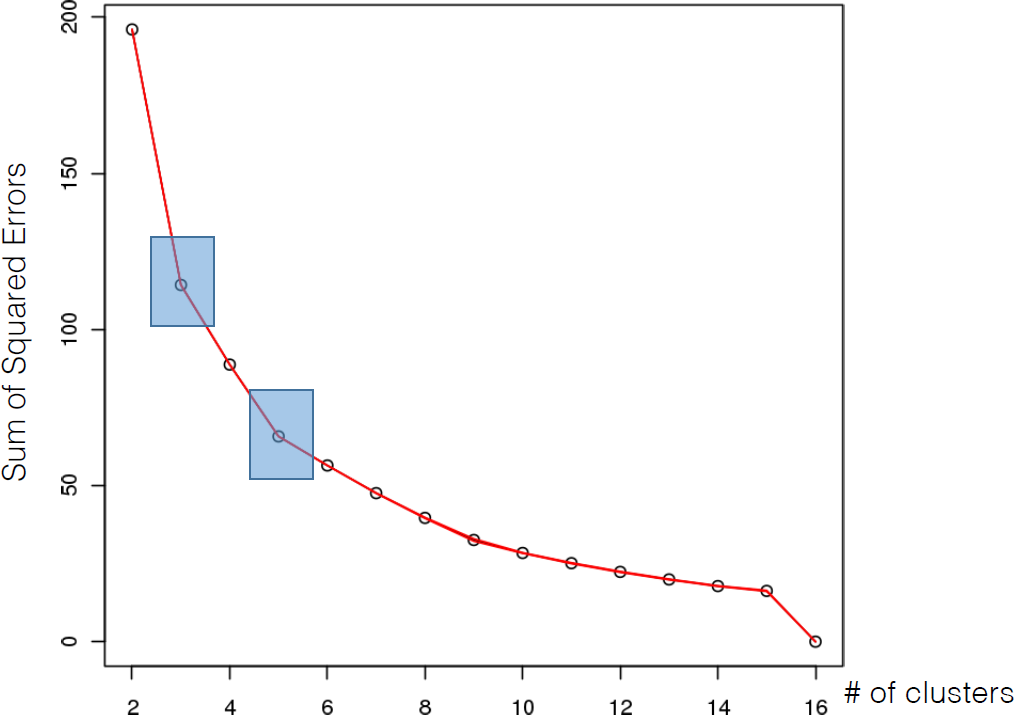
\includegraphics[width=0.40\textwidth]{images/DSML/clustering19.png} \caption[\small Optimal clustering results for the iris dataset: DBI, SSE]{\small Optimal clustering results for the iris dataset: 5 clusters using (modified) Davies-Bouldin index and Sum of Squared Errors.}\label{fig:clust1819}
\end{figure}
\afterpage{\FloatBarrier}
\begin{figure}[!t]
\centering
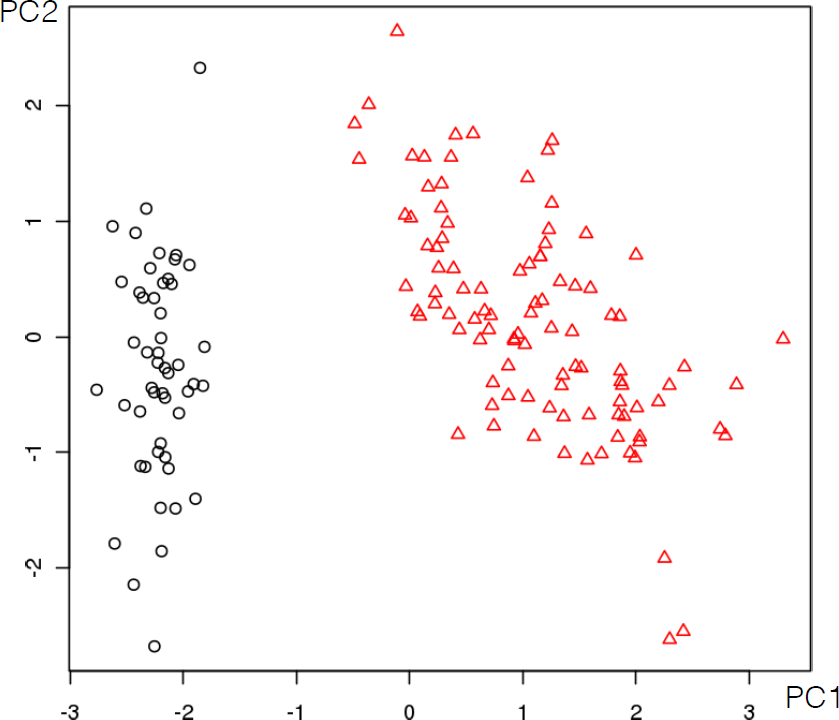
\includegraphics[width=0.45\textwidth]{images/DSML/clustering14.png}\quad 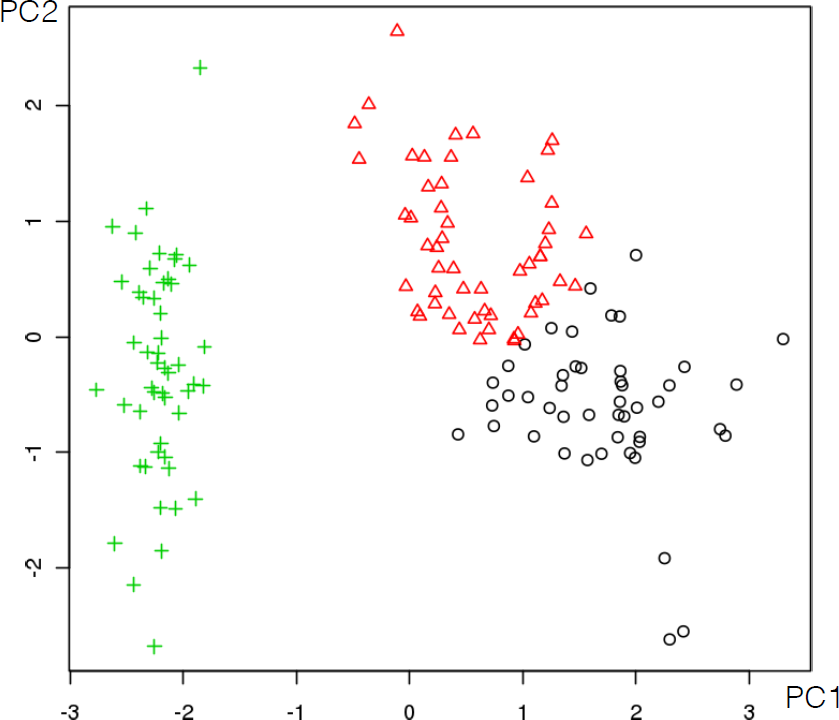
\includegraphics[width=0.45\textwidth]{images/DSML/clustering15.png} \\ 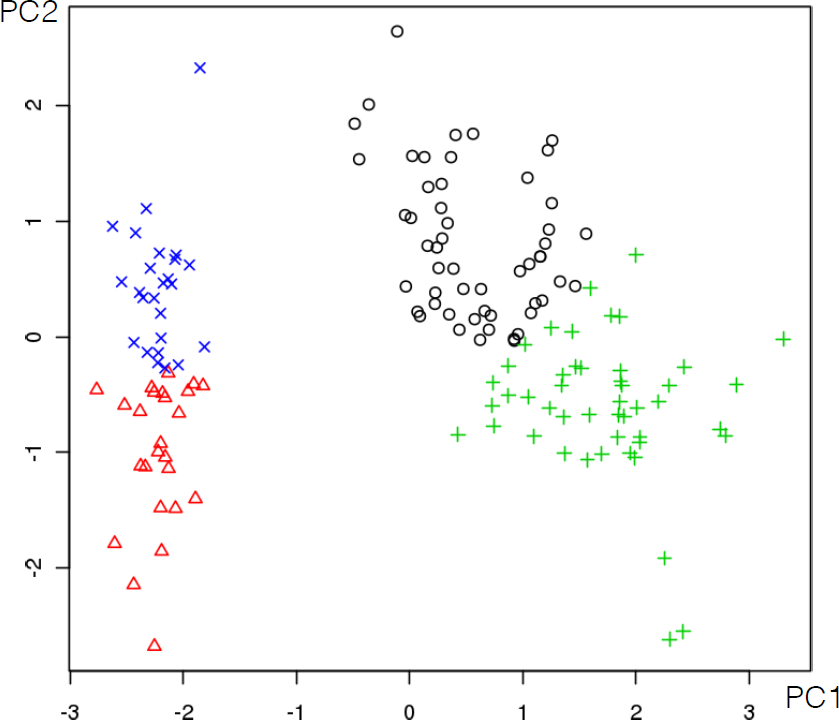
\includegraphics[width=0.45\textwidth]{images/DSML/clustering16.png} \quad 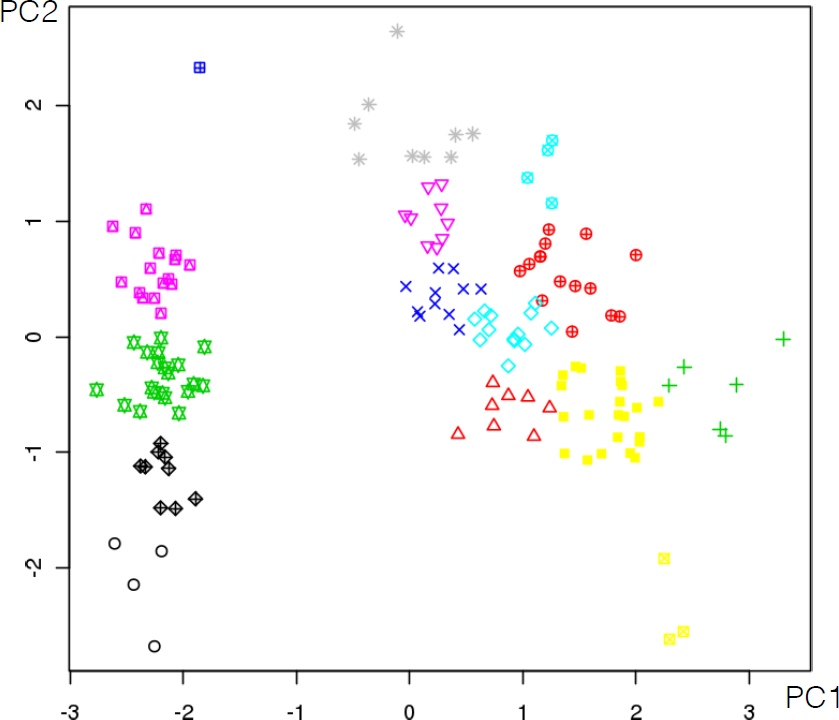
\includegraphics[width=0.45\textwidth]{images/DSML/clustering17.png}
\caption[\small Clustering results on the iris dataset]{\small Clustering results on the iris dataset with $k-$means, for $k=2,3,4,15$ (from top left to bottom right, by row). }\label{fig:clust14151617}
\end{figure}
\afterpage{\FloatBarrier}

\begin{figure}[!t]
\centering
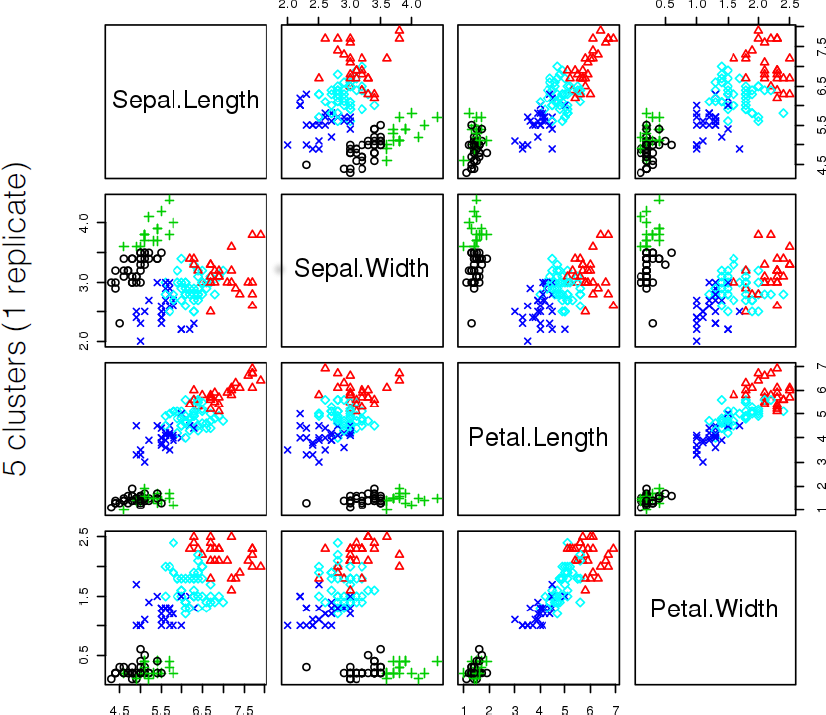
\includegraphics[width=0.8\textwidth]{images/DSML/clustering20.png} \caption[\small Optimal clustering results for the iris dataset: visualisation]{\small Optimal clustering results for the iris dataset: visualisation.}\hrule\label{fig:clust20}
\end{figure}
\afterpage{\FloatBarrier}
\newpage\noindent
\subsubsection{Issues and Challenges}
\begin{tcolorbox}[title=The Stench of Bad Data]
We all say we like data, but we don't. We like getting insight out of data. That's not quite the same as liking data itself. In fact, I dare say that I don't quite care for data, and it sounds like I'm not alone. \\[-0.6cm]
\begin{flushright}
-- Q.E. McCallum, \textit{Bad Data Handbook}
\end{flushright}
\end{tcolorbox}
\noindent The data science landscape is littered with issues and challenges. Here are a few of them. 
\paragraph{Bad Data}
We have touched upon data collection and data cleaning in Sections~\ref{sec:DC} and \ref{sec:DP} and mentioned some of the most common data issues, namely that the available data is not always \textbf{representative} of the situation that the client would like to see modeled, and that it might not be sound. There are other potential issues, such as \cite{DSML_BDH}:
\begin{itemize}[noitemsep]
\item the data might formatted for human consumption, not machine readability;
\item the data might contain lies and mistakes;
\item the data might not reflect reality;
\item there might be additional sources of bias and errors (not only imputation bias, but replacing extreme values with average values, proxy  reporting, etc.);
\item seeking perfection in the data can hamper the efforts of clients and consultants alike; there are different quality requirements for academic data, professional data, government data, military data, service data, commercial data, etc. -- remember the engineering dictum: ``close enough is good enough'' (in terms of completeness, coherence, correctness, and accountability).
\end{itemize}
These accompany the \textbf{data analysis pitfalls}: 
\begin{itemize}[noitemsep]
\item analysing data \textbf{without understanding it}, or the context;
\item using \textbf{one and only one tool} (by choice or by fiat) -- neither the cloud nor Big Data will solve all of the client's problems!;
\item analysing data for the sake of analysis;
\item having \textbf{unrealistic expectations} of data analysis -- consultants must bear some of the blame for this... don't oversell!
\end{itemize}
\paragraph{Overfitting}
In a traditional statistical model, $p-$values (or other statistics) can help validate how good a model is. For predictive data science models, such statistics cannot usually be computed. We recognise a ``good'' model based on how well it performs on unseen data. In practice, then, we hope for rules and models generated by data science techniques on a training set to be \textbf{generalisable to new data} (or validation/ testing sets). \newl Problems arise when knowledge that is gained from supervised learning does not generalize properly to the data. Ironically, this may occur if the rules or models fit the training set too well -- the results are too specific to the training set (see Figure~\ref{fig:uoj}) for an illustration of \textbf{overfitting} and \textbf{underfitting}).
\begin{figure}[!t]
\centering
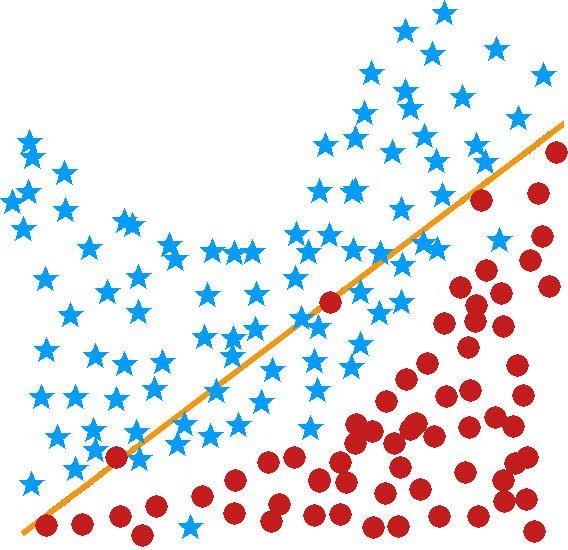
\includegraphics[width=0.3\textwidth]{images/DSML/underfit.png} \quad 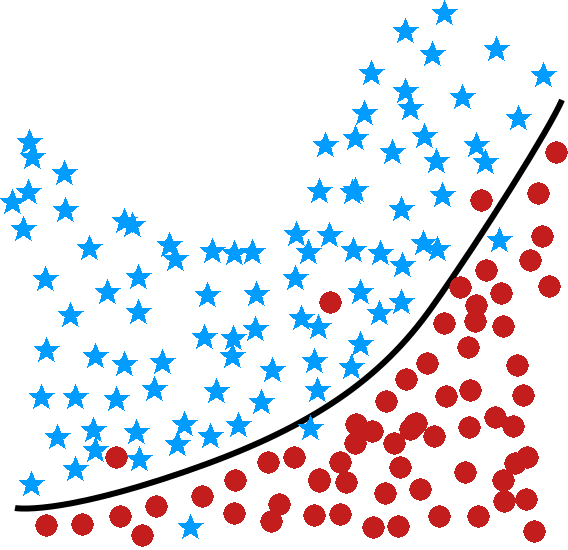
\includegraphics[width=0.3\textwidth]{images/DSML/justright.png} \quad 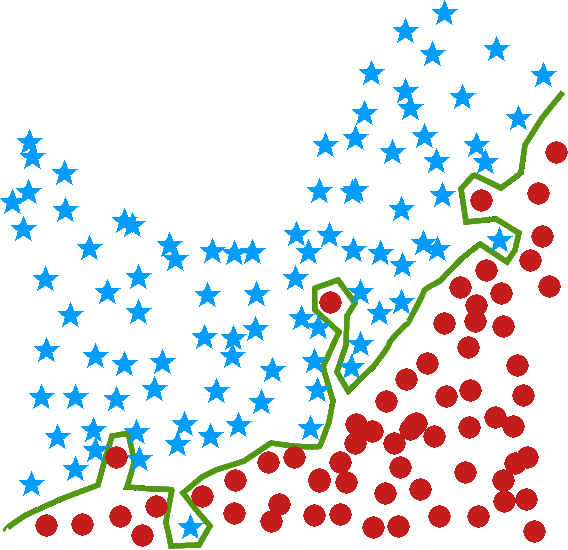
\includegraphics[width=0.3\textwidth]{images/DSML/overfit.png}
 \caption[\small An illustration of underfitting and overfitting]{\small An illustration of underfitting (left) and overfitting (right); a reasonable fit is shown in the middle.}\label{fig:uoj}
\end{figure}
\afterpage{\FloatBarrier}
\newpage\noindent A simple example may elucidate further. Consider the following set of rules regarding hair colour among humans: 
\begin{itemize}[noitemsep]
\item \textbf{vague rule} -- some people have black hair, some have brown hair, some blond, and some red (this underfit rule is probably too general to be useful);
\item \textbf{reasonable rule} -- in populations of European descent, approximately 45\% have black hair, 45\% brown hair, 7\% blond and 3\% red;
\item \textbf{overly specific rule} -- in every group of 100 individuals of European descent, we predict that there will be 46.3\% with black hair, 47.2\% with brown hair, 6.5\% with blond hair, and 0\% with red hair (this overfit rule is presumably based on some training set data without redheads). 
\end{itemize}
With the overfit rule, we would predict that there are no redheads in populations of European descent, which is blatantly false. This result is simply specific to the particular training subset that was used -- it was not representative of the entire dataset (assuming that the dataset itself was representative of the population of interest). \newl More formally, underfitting and overfitting can be viewed as resulting from the level of model complexity (see Figure~\ref{fig:uomc}).  
\begin{figure}[!t]
\centering
\includegraphics[width=0.7\textwidth]{images/DSML/overunder.png} \caption[\small Underfitting and overfitting as a function of model complexity]{\small Underfitting and overfitting as a function of model complexity; error prediction on training sample (blue) and testing sample (red). High error prediction rates for simple models are a manifestation of underfitting; large difference between error prediction rates on training and testing samples for complex models are a manifestation of overfitting. Ideally, model complexity would be chosen to reach the situation's ``sweet spot'', but fishing for the ideal scenario might diminish explanatory power (based on \cite{DSML_HTF}).}\label{fig:uomc}
\end{figure}
\afterpage{\FloatBarrier}
Overfitting can be overcome in several ways:
\begin{itemize}[noitemsep]
\item \textbf{using multiple training sets}, with overlap being allowed -- this has the effect of reducing the odds of finding spurious patterns based on quirks of the training data;  
\item \textbf{using larger training sets} may also remove signal which is too specific to a small training set -- a 70\% - 30\% split is  often suggested.
\end{itemize}
Depending on the size of the data, there are different guidelines: when faced with 
\begin{itemize}[noitemsep]
\item \textbf{small datasets} (less than a few hundred observations, say, but that depends on numerous factors such as computer power and number of tasks), use 100-200 repetitions of a \textbf{bootstrap procedure};
\item \textbf{average-sized datasets} (less than a few thousand observations), use a few repetitions of 10-fold cross-validation (see Figure~\ref{fig:cv1});
\item \textbf{large datasets}, use a few repetitions of a holdout split (70\%-30\%, say).
\end{itemize}
\textbf{IMPORTANT NOTE:} remember to always, always (always!) evaluate the models on unseen data.
\begin{figure}[!t]
\centering
\includegraphics[width=\textwidth]{images/DSML/8-4fcv.png} \caption[\small Illustration of cross-fold validation]{\small Schematic illustration of cross-fold validation, for 8 replicates and 4 folds; $8\times 4=32$ models from a given family are built on various training sets (consisting of $3/4$ of the available data -- the training folds). Model family performance is evaluated on the respective holdout folds; the distribution of the performance metric values (in practice, some combination of the mean/median and standard deviation) can be used to compare various model families  (based on \cite{DSML_PF,DSML_T}).}\hrule\label{fig:cv1}
\end{figure}
\afterpage{\FloatBarrier}
\paragraph{Appropriateness and Transferability}
Data science models will be used heavily in the coming years (in fact, it has already started). We have discussed pros and cons of some of the applications on ethical and other non-technical grounds, but there are also \textbf{technical challenges}. In general, data science methods may \textbf{not} be appropriate if: 
\begin{itemize}[noitemsep]
\item you absolutely must use an existing (legacy) datasets instead of an ideal dataset (the dreaded ``it's the best data we have!'' response);
\item the dataset has attributes that usefully predict a value of interest, but these attributes are not available at the time when a prediction is required (e.g. the total time spent on a website may be predictive of a visitor's future purchases, but the prediction must be made before the total time spent on the website is known);
\item you will attempt to predict class membership using an unsupervised learning algorithm (e.g. clustering loan default data might lead to a cluster contains many defaulters. If new instances get added to this cluster, should they automatically be viewed as loan defaulters?) 
\end{itemize}
Every model makes certain assumptions about what is and is not \textbf{relevant} to its workings, but there is a tendency to only gather data which is \textbf{assumed} to be relevant to a particular situation. If data is used in other contexts, or to make predictions depending on attributes for which no data is available, then there might be no way to validate the results (e.g. can we use a model that predicts whether a borrower will default on a mortgage or not to also predict whether a borrower will default on a car loan or not? The problem is compounded by the fact that there might be some link between mortgage defaults and car loan defaults, but the original model does not necessarily takes this into account). The problem is less academic than it might appear: \textbf{over-generalisations and inaccurate predictions can lead to harmful results}.
\paragraph{Myths and Mistakes}
We end this section with a short discussion of various data science (DS) myths and mistakes (based on \cite{DSML_CL13}, but they apply to quantitative consulting as a whole).
\begin{itemize}[noitemsep]
\item Myth \#1: DS is about algorithms
\item Myth \#2: DS is about predictive accuracy
\item Myth \#3: DS requires a data warehouse
\item Myth \#4: DS requires a large quantity of data
\item Myth \#5: DS requires technical experts
\item Mistake \#1: selecting the wrong problem
\item Mistake \#2: getting buried under tons of data without metadata understanding.
\item Mistake \#3: not planning the data analysis process
\item Mistake \#4: insufficient business and domain knowledge
\item Mistake \#5: using incompatible data analysis tools
\item Mistake \#6: using tools that are too specific
\item Mistake \#7: ignoring individual predictions/records in favour of aggregated results
\item Mistake \#8: running out of time
\item Mistake \#9: measuring results differently than the sponsor
\item Mistake \#10: na\"{\i}vely believing what one is told about the data
\end{itemize}
\textbf{IMPORTANT NOTE:} it is your responsibility as a consultant to address these issues with the client. Do not assume that you are all on the same page -- prod and ask.  
\subsubsection{The Rest of the Data Science Picture}
Even by the standards of this work, we have only scratched the surface of data science methods and tasks. In this section, we will briefly introduce a number of other related concepts. More information can be found in the references. 
\paragraph{A.I. and Neural Networks}
\begin{figure}[!t]
\centering
\includegraphics[width=0.75\textwidth]{images/DSML/AIDL1.png} \caption[\small A.I. Timeline (1950-20??)]{\small Conceptual timeline of the interest and optimism regarding artificial intelligence (A.I.); important milestones are indicated below the dates.}\hrule\label{fig:aidltimeline}
\end{figure}
\afterpage{\FloatBarrier}
\ \newline
\begin{tcolorbox}[title=Deep Learning Indeed]
Neural networks blow all previous techniques out of the water in terms of performance, but given the existence of adversarial examples, it shows we really don't understand what's going on.
 \\[-0.6cm]
\begin{flushright}
-- D. Gershgorn, \textit{Quartz}
\end{flushright}
\end{tcolorbox}
\noindent At various times since Alan Turing's seminal 1950 paper (in which he proposed the famous \textit{Imitation Game} \cite{DSML_AI9}), complete artificial intelligence has been announced to be ``just around the corner'' (see A.I winters, Figure~\ref{fig:aidltimeline}). With the advent of \textbf{deep learning} and Big Data processing, optimism is as high as it's ever been. At the very least, it seems to be the topic \textit{du jour}. Case in point, consider the following four recent headlines: 
\begin{itemize}[noitemsep]
\item ``AlphaGo vanquishes world's top Go player, marking A.I.'s superiority over human mind'' [South China Morning Post, May 27, 2017]
\item ``A Japanese A.I. program just wrote a short novel, and it almost won a literary prize'' [Digital Trends, March 23, 2016]
\item ``Elon Musk: Artificial intelligence may spark World War III'' [CNET, September 4, 2017]
\item ``A.I. hype has peaked so what's next?'' [TechCrunch, September 30, 2017]
\end{itemize}
\newpage\noindent Opinions
\begin{figure}[!t]
\centering
\includegraphics[width=0.8\textwidth]{images/DSML/AIDL3.png} \caption[\small ANN topology]{\small Artificial neural network topology -- conceptual example. The number of hidden layers is arbitrary, as is the size of the signal and output vectors.}\hrule\label{fig:aidl3}
\end{figure}
\afterpage{\FloatBarrier}
 on the topic are varied -- to some commentators, A.I. is both a brilliant success while to others it is a spectacular failure. What is A.I. and what is going on?
\begin{center}\rule{0.5\linewidth}{.4pt}\end{center}
According to \cite{DSML_GEB}, the \textbf{essential qualities and skills of an intelligence} are that it:
\begin{itemize}[noitemsep]
\item provides flexible responses in various scenarios;
\item takes advantage of lucky circumstances;
\item makes sense out of contradictory messages;
\item recognises the relative importance of a situation's elements;
\item finds similarities between different situations;
\item draws distinctions between similar situations, and 
\item comes up with new ideas from scratch or by re-arranging previous known concepts.
\end{itemize}
A.I. research is defined as the study of \textit{intelligent agents} -- any device that perceives its environment and takes actions to maximise its chance of success at some task/goal \cite{DSML_AIW}. Examples include 
\begin{itemize}[noitemsep]
\item \textbf{expert systems} -- TurboTax, WebMD, technical support, insurance claim processing, air traffic control, etc.;
\item \textbf{decision-making} -- Deep Blue, auto-pilot systems, ``smart'' meters, etc.;
\item \textbf{natural Language Processing} -- machine translation, Siri, named-entity recognition, etc.;
\item \textbf{recommenders} -- Google, Expedia, Facebook, LinkedIn, Netflix, Amazon, etc.;
\item \textbf{content generators} -- music composer, novel writer, animation creator, etc.;
\item \textbf{classifiers} -- facial recognition, object identification, fraud detection, etc.
\end{itemize}
A trained \textbf{artificial neural network} (ANN) is a function that maps inputs to outputs in a useful way: it uses a Swiss-army-knife approach to providing outputs -- plenty of options are available in the \textbf{architecture}, but it's not always clear which ones should be used. One of the reasons that ANNs are so popular is that the user does not need to decide much about the function or know much about the problem space in advance -- ANNs are \textbf{quiet models}.\par Algorithms allow ANNs to \textbf{learn} (i.e. to generate the function and its internal values) automatically; technically, the only requirement is the ability to minimise a cost function (optimisation).
\begin{center}\rule{0.5\linewidth}{.4pt}\end{center}
ANNs are formed from an \textbf{input layer} from which the \textbf{signal vector} $x$ is inputted, an \textbf{output layer} which produces an \textbf{output vector} $\hat{y}$, and any number of \textbf{hidden layers}; each layer consists of a number of \textbf{nodes} which are connected to the nodes of other layers \textit{via} \textbf{directed edges} with associated \textbf{weights} $w$ (see Figure~\ref{fig:aidl3}). Nodes from the hidden and output layers are typically \textbf{activation nodes} -- the output $a(z)$ is some function of the input $z$. Signals propagate through the ANN using simple arithmetic, once a set of weights $\mathbf{w}$ and activation functions $\mathbf{a(\cdot)}$ have been selected (see Figure~\ref{fig:aidlprop}). In a nutshell, at each node, the neural net
computes a weighted sum of inputs, applies an activation function, and sends a signal. This is repeated until the various signals reach the final output nodes.\par That part is easy -- given a signal, an ANN can produce an output, as long as the weights are specified. Matrix notation can simplify the expression for the output $\hat{y}$ in terms of the signal $x$, weights $w$, and activation function $a(\cdot)$. For instance, consider the network of Figure~\ref{fig:aidl3}; if $a(z)=$, the network topology can be re-written as  
\begin{center}
\includegraphics[width=0.8\textwidth]{images/DSML/inputtohidden.png}\\[0.3cm]
\includegraphics[width=0.8\textwidth]{images/DSML/hiddenttooutput.png}
\end{center}
from which we conclude that the output is 
\begin{center}
\includegraphics[width=0.6\textwidth]{images/DSML/output.png} .
\end{center}
The problem is that unless the weights are judiciously selected, the output that is produced is unlikely to have anything to do with the desired output. For supervised learning tasks (i.e. when an ANN attempts to emulate the results of training examples), there has got to be some method to optimise the choice of the weights against an error function $$R(W)=\sum_{i=1}^n\sum_{k=1}^K\left(\hat{y}_{ik}(W)-y_{ik}\right)^2\quad\mbox{or}\quad R(W)=-\sum_{i=1}^n\sum_{k=1}^Ky_{ik}\ln \hat{y}_{ik}(W)$$ (for value estimation and classification, respectively), where $n$ is the number of observations in the training set, $K$ is the number of output nodes in the ANN, $y_{ik}$ is the known value or class label for the $k^{\textrm{th}}$ output of the $i^{\textrm{th}}$ observation in the training set -- enter \textbf{backpropagation}, which is simply an application of the chain rule to $R(W)$ (the minimum is then found using numerical gradient descent). 
\begin{figure}[!t]
\centering
\includegraphics[width=0.48\textwidth]{images/DSML/AIDL5.png} \includegraphics[width=0.48\textwidth]{images/DSML/AIDL6.png}
\includegraphics[width=0.48\textwidth]{images/DSML/AIDL7.png} \includegraphics[width=0.48\textwidth]{images/DSML/AIDL8.png}
\caption[\small Feed forward network]{\small Signal propagating forward through an ANN; weights (in blue) and activation functions (in yellow) are given; inputs (in green), output (in black). }\hrule\label{fig:aidlprop}
\end{figure}
\afterpage{\FloatBarrier}
\begin{center}\rule{0.5\linewidth}{.4pt}\end{center}
ANNs can be quite accurate when making predictions -- more than other algorithms, if given a proper set up (which can be hard to achieve). They degrade gracefully, and they often work when other things fail:
\begin{itemize}[noitemsep]
\item when the relationship between attributes is \textbf{complex};
\item when there are a lot of dependencies/\textbf{nonlinear relationships};
\item when the inputs are \textbf{messy} and highlyconnected (images, text and speech), and
\item when dealing with non-linear classification
\end{itemize}
On the other hand, they are relatively slow and prone to overfitting (unless they have access to  large and diverse training sets). They are notoriously hard to interpret due to their \textbf{blackbox} nature, and there is no algorithm in place to select the optimal network topology. Finally, even when Even when they do perform better than other options, ANNs may not perform that much better due various \textbf{No Free-Lunch} theorems; and they are susceptible to various forms of adversarial attacks.
\paragraph{Text Mining and Natural Language Processing}\ \newline
\begin{tcolorbox}[title=Language and Data]
Q: How many legs does a cat have if you call the tail a leg?\newline
A: Four. Calling the tail a leg doesn't make it a leg.
 \\[-0.6cm]
\begin{flushright}
-- Old riddle, attributed to A. Lincoln
\end{flushright}
\end{tcolorbox}
\noindent In this document, we take the position that \textbf{text mining} is the application of the typical data science tasks to text documents, with applications to \textbf{authorship questions} (classification), \textbf{sentiment analysis} (value estimation), \textbf{taxonomy creation} and \textbf{topic modeling} (clustering), \textbf{text description}, and \textbf{text visualisation}. \par \textbf{Natural language processing} (NLP), in contrast, has a long history of lofty goals, which more or less boil down to developing machines that react ``appropriately'' while interacting with (natural) human languages. The focus of NLP tasks tends towards ``understanding'' languages; with common tasks including 
\begin{itemize}[noitemsep]
    \item \textbf{syntax} (lemmatization, part-of-speech tagging, parsing, terminology extraction, sentence boundary disambiguation, stemming, word segmentation, etc.)
    \item \textbf{semantics} (machine translation, language generation, named entity recognition, optical character recognition, questions and answers, sentiment analysis, textual entailment, topic segmentation, word sense disambiguation, etc.)
    \item \textbf{discourse} (coreference resolution, discourse analysis, summarization, etc.)
    \item \textbf{speech} (recognition, segmentation, text-to-speech, etc.) \cite{TM_NLP_W}
\end{itemize}
Most natural human languages rules are dynamic, and usage may change drastically in space and time -- a \textit{poutine} is not the same delicious dish in New Brunswick as it is in Qu\'ebec, for instance (see Figure~\ref{fig:poutine})
\begin{figure}\centering \includegraphics[width=\textwidth]{images/DSML/poutines.png}\caption[\small Poutines]{\small A poutine (left); an abomination in the eyes of all right-thinking sentient beings (right).}\label{fig:poutine} \end{figure} For another example, consider the meaning of the word \textit{awful}, which drifted from  
\begin{quote}
``worthy of, or commanding, profound respect or reverential fear'' to ``frightful, very ugly, monstrous''
\end{quote}
from 1000 AD onward. Other issues arise from dialect variations and individual-specific speech patterns, either due to linguistic drift, influence from other languages, sarcasm, idioms, figures of speech, and so forth. The intended meaning is often clear to experienced human speakers based on the specific context, but it is believed that natural language understanding is \textbf{AI-hard}  -- a complete resolution of the issues would require the ability to make computers as humans \cite{TM_IV}. \par Thankfully, we rarely need a resolution at the most general level; in many areas, the current state of the art produces results which are acceptable to a large class of users. Since the 1990s, the NLP community has adopted a machine learning paradigm, which has provided advantages over the classical hard-coded hand-produced rules. Statistical machine translation, for instance, can take advantage of domain constraints and formal language habits to reduce the space of outputs and produce accurate translations of technical documents \cite{TM_WG}.  
\newl Let us take a look at two schools of thought regarding text mining: \textbf{semantic parsing} (SM) and \textbf{bag-of-words} (BoW) mining. \newpage\noindent In the SM view of text mining, word order and word type play a crucial role. The idea is to use a large number of hand-parsed sentences to train a model that outputs the most likely grammatical analysis of a sentence. Words are tagged along a tree structure, and may have multiple features. This information can then be used to extract insights about the sentence or document. \newl For instance, consider the sentence \begin{quote}(S1) Dzingel added to the lead when he deflected Marc Methot's point shot 20 seconds later \cite{TM_OTT_TOR},\end{quote} a syntactic parsing of which is shown in Figure~\ref{fig:sent_pars2} (the output of the Stanford parser \cite{TM_SP}); \begin{figure}[!t]\centering\includegraphics[width=\textwidth]{images/DSML/TMSemanticParsing.png}\caption[\small Syntactic parsing tree]{\small Syntactic parsing of a sentence using the Stanford parser \cite{TM_SP}.}\hrule\label{fig:sent_pars2}\end{figure} another display is provided in Figure~\ref{fig:tree2}.
\begin{figure}[!t]
\centering\footnotesize \begin{verbatim}
(ROOT
 (S
  (NP (NNP Dzingel))
  (VP (VBD added)
    (PP (TO to)
      (NP (DT the) (NN lead)))
    (SBAR
      (WHADVP (WRB when))
      (S
        (NP (PRP he))
        (VP (VBD deflected)
          (NP
            (NP (NNP Marc) (NNP Methot)
                            ... (POS 's))
            (NN point) (NN shot))
          (ADVP
            (NP (CD 20) (NNS seconds))
            (RB later))))))))
\end{verbatim}
\normalsize
\caption[\small Secondary view of syntactic parsing]{\small Secondary view of syntactic parsing tree.}\hrule\label{fig:tree2}
\end{figure}
From the tree diagram, a human observer can clearly see that ``Marc Methot'' is correctly parsed as a \textit{noun phrase} (NP), that the ``'s'' is correctly identified as a \textit{possessive marker} (POS), and that ``Marc Methot's point shot'' is correctly shown as a NP (built from 2 \textit{singular proper nouns}, NNP), but the parser fails to recognize  ``point shot'' as an NP. The two displays are, of course, equivalent. A computer program can be used to easily go from one to the other; a human with the right experience would find both as insightful. But it's certainly easier for a neophyte to comprehend the tree diagram. Why is that? Is it simply because we are a visual species? Or because most of us have parsed sentence fragments in our native languages as youths? In another parsing (using the Enju parser), ``Marc Methot's point shot 20 seconds later'' is tagged as a \textit{simple declarative clause} (S), but ``Marc Methot's point'' and ``shot 20 seconds later'' are wrongly identified as a NP and a \textit{verb phrase} (VP), respectively, underscoring the importance of parsing to our understanding of a sentence.  
\newl The \textbf{part-of-speech tagging} for the sentence is shown in the table below: 
\begin{center}\begin{tabular}{cc|cc} \hline
\textbf{Word} & \textbf{Tag} & \textbf{Word} & \textbf{Tag} \\ \hline
Dzingel & NNP &  Marc & NNP\\
added & VBD & Methot & NNP \\
to & TO & 's & POS \\ 
the & DT & point & NN \\ lead & NN & shot & NN\\ when & WRB & 20 & CD \\ he & PRP & seconds & NNS \\ deflected & VBD  & later & RB \\ \hline \end{tabular}\end{center} Notice how relational insight between the parts-of-speech has gotten lost (or is not displayed, at the very least).\newl 
The Stanford parser also provides a list of \textbf{universal dependencies}: 
\begin{itemize}[noitemsep]
\item nsubj(added-2, Dzingel-1)
\item root(ROOT-0, added-2)
\item case(lead-5, to-3)
\item det(lead-5, the-4)
\item nmod(added-2, lead-5)
\item advmod(deflected-8, when-6)
\item nsubj(deflected-8, he-7)
\item advcl(added-2, deflected-8)
\item compound(Methot-10, Marc-9)
\item nmod:poss(shot-13, Methot-10)
\item case(Methot-10, 's-11)
\item compound(shot-13, point-12)
\item dobj(deflected-8, shot-13)
\item nummod(seconds-15, 20-14)
\item nmod:npmod(later-16, seconds-15)
\item advmod(deflected-8, later-16)
\end{itemize}
For instance, ``he'' (the 7th token in the sentence) is the \textit{nominal subject} (nsubj) of ``deflected'' (the 8th token), ``point shot'' is recognised as a \textit{compound}, and ``shot'' (the 13th token) is the \textit{direct object} (dobj, the second most core argument of a verb after the subject) of ``deflected'' (the 8th token).
\newl In the BoW view of text mining, only the words are important -- it is frequency (and relative frequency) that wins the day. In semantic parsing, the words have attributes depending on their position and role in the document's sentences; in bag of words analysis, \textbf{the words themselves are attributes of the document}. Our sentence S1 is simply a collection of words, arranged here alphabetically: 
\begin{quote}
's, 20, added, deflected, Dzingel, he, later, lead, Marc, Methot, point, seconds, shot, the, to, when.  
\end{quote}
The fact that ``point shot'' is a noun phrase is not significant, but the fact that ``point'' and ``shot'' appear in the list is significant -- it is the \textbf{relative frequencies} of the terms that provide information about the document or collection of documents (such as intent and themes). \begin{center}\rule{0.5\linewidth}{.4pt}\end{center}
No matter where text data comes from and what analyses we hope to run on it, the crucial first step requires extraction, formatting, and storage to a data structure with appropriate numerical properties:  \begin{itemize}[noitemsep] 
\item a \textbf{string} or vector of characters, with language-specific encoding;
\item a collection of text documents (with meta information) called a \textbf{corpus} (`permanent' when stored on disk; `volatile' when held in RAM); 
\item a \textbf{document-term matrix} (DTM) -- or the transposed \textbf{term-document matrix} (TDM) -- where the rows are the documents, the columns are the terms (see Figure~\ref{fig:TDM}), and the entries represent some text statistic;
\item a \textbf{tidy text dataset} containing one \textbf{token} (single word, $n$-gram, sentence, paragraph) per row. 
\end{itemize}
The DTM/TDM \textbf{representations} are \textbf{essential} to any statistical analysis of text data  -- it is on these entities that machine learning  algorithms are unleashed. \newl 
Like every form of data, text data requires extensive cleaning and processing. Cleaning text data is, to put it mildly, even less pleasant a process than cleaning numeric or categorical data. There are  challenges due to the nature of the data: how would one go about finding anomalies in the text? Outliers? Is the concept even definable for text data? \par Character \textbf{encoding} may also produces surprises: a text (or a part of text) that looks completely normal to the naked eye may be unreadable to a computer because it was expecting a different coding system. There are probabilistic ways to detect a document's encoding, and ways to coerce a specified encoding -- if you are working with text data and your code balks at doing something it should be able to do and none of the usual fixes apply, look into the encoding situation.  
\par Another issue is that spelling mistakes and typographical errors are hard to catch in large documents (even with spell-checkers), to say nothing of:
\begin{itemize}[noitemsep]
\item accent representation (\textit{ya new cah's wicked pissa!});
\item neologisms and portmanteaus (\textit{ruthfull}; \textit{can't you tell that I'm planning prevenge?});
\item poor translations or foreign words (\textit{I dou not spik inglishe}; \textit{llongyfarchiadau});
\item puns and play-on-words (\textit{they were yung and easily freudened!});
\item specialized vocabulary (\textit{clopen}; \textit{poset}); 
\item fictional names and places (\textit{Qo'noS}; \textit{Kilgore Trout});
\item slang and curses (\textit{skengfire}; \textit{\#\$\&\#!});
\item mark-up and tags (\textit{<b>}; \textit{{$\backslash$}includegraphics});
\item uninformative text information (page number; ISBN blurb), etc. 
\end{itemize} 
The process can be simplified to some extent with the help of \textbf{regular expressions} and \textbf{text pre-processing functions} to: \begin{itemize}[noitemsep]
\item convert all letters to \textbf{lower case}, which should be avoided when seeking proper names;
\item remove all \textbf{punctuation marks}, which should be avoided when seeking emojisl
\item remove all \textbf{numerals}, which should be avoided when mining for quantities; 
\item remove extraneous \textbf{white spaces};
\item remove characters withing \textbf{brackets}, which should be avoided when seeking tags;
\item replace all \textbf{numeral with words}, etc. 
\end{itemize}
\begin{table}[!t]
\centering
\includegraphics[width=\textwidth]{images/DSML/TDM.png}
\caption[\small TDM/DTM for a hypothetical corpus]{\small Term-Document Matrix / Document-Term Matrix for a hypothetical corpus, with row sums and column sums.}\hrule\label{fig:TDM}
\end{table}
\begin{center}\rule{0.5\linewidth}{.4pt}\end{center}
The purest BoW information about a term $t$ in a document $d$ is the raw \textbf{term frequency count} $\textrm{tf}_{t,d}$. Other measures are also used, such as the \textbf{relative term frequency}  (or term proportion) $$\textrm{tf}^*_{t,d}=\frac{\textrm{tf}_{t,d}}{M_{d}},$$ the \textbf{relative document frequency} $$\textrm{df}^*_{t}=\frac{\sum_d\textrm{sign}\left(\textrm{tf}_{t,d}\right)}{N}$$ or the \textbf{term frequency-inverse document frequency} $$\textrm{tf-idf}_{t,d}=-\textrm{tf}^*_{t,d}\times \ln \textrm{df}^*_{t},$$ where $M_d$ is the number of retained terms in sentence $d$, and $N$ is the number of documents in the corpus. 
If \textbf{all the corpus' documents} contain the term $t$, then $\textrm{df}^*_{t}=1$ and $$\textrm{tf-idf}_{t,d} = -\textrm{tf}^*_{t,d}\times \ln 1 =0,$$ which is to say that this specific term does not provide information in the tf-idf framework. If a term $t$ \textbf{rarely occurs} in a document $d$, then  $\textrm{tf}^*_{t,d}\approx 0$ and $$\textrm{tf-idf}_{t,d} \approx 0 \times \ln \textrm{df}^*_{t} =0.$$ Terms that appear relatively often only in a small subset of documents are crucial to understanding those documents in the general context of the corpus -- that's the interpretation of the tf-idf statistic (although we hasten to add that this argument is not rigorous and is considered at best a heuristic by many practitioners). 
\newl The following example provides an illustration of the various \textbf{text statistics}. 
\par Consider a corpus $\mathcal{C}=\{d_1,\ldots,d_3\}$ consisting of of the following 3 documents:\begin{quote} $d_1=$``the dogs who have been let out'', $d_2=$``who did that?'', and $d_3=$``my dogs breath smells like dogs food'' [sic].\end{quote} Suppose that after processing, the following 14 terms are retained: 
\begin{quote}
$t_1=$``been'', $t_2=$``breath'', $t_3=$``did'', $t_4=$``dogs'', $t_5=$``food'', $t_6=$``have'', $t_7=$``let'', $t_8=$``like'', $t_9=$``my'', $t_{10}=$``out'', $t_{11}=$``smells'', $t_{12}=$``that'', $t_{13}=$``the'', and $t_{14}=$``who''. 
\end{quote}
\newpage\noindent The text statistics of this corpus are shown in Table~\ref{tab:tfs}.
\begin{table}[!t]
\centering
\begin{subtable}[c]{\textwidth}
\includegraphics[width=\textwidth]{images/DSML/TMTF.png}\caption{\small Relative term frequency}\label{tab:tmtf}
\end{subtable}
\begin{subtable}[c]{\textwidth}
\includegraphics[width=\textwidth]{images/DSML/TMDF.png}\caption{\small Relative document frequency}\label{tab:tmdf}
\end{subtable}
\begin{subtable}[c]{\textwidth}
\includegraphics[width=\textwidth]{images/DSML/TMTFIDF.png}\caption{\small Term frequency -- inverse document frequency}\label{tab:tmtfidf}
\end{subtable}\caption[\small Illustration of text statistics]{\small Illustration of text statistics on the toy corpus $\mathcal{C}$.}\hrule \label{tab:tfs}
\end{table}
Of course, the choice of a text statistic will have an effect on the numerical representation of the corpus, and so on the analytical results that are produced. 
\begin{center}\rule{0.5\linewidth}{.4pt}\end{center}
Let us take a look at one specific text mining task. Most of us have a good native understanding of the emotional intent of words, which leads us to infer \textbf{surprise}, \textbf{disgust}, \textbf{joy}, \textbf{pain} (and so forth) from a text segment. The process, when applied by machines to a block of text, is known as \textbf{sentiment analysis} (or opinion mining), and it used to answer questions such as:
\begin{itemize}[noitemsep]
\item ``Is this movie review positive or negative?''
\item ``Is this customer email a complaint?''
\item ``Have newspapers' attitudes about the Prime Minister changed since the election?''
\end{itemize}
Most humans would typically be able to answer these questions when presented with the appropriate text documentation. But there are challenges, which we may have a difficult time translating into the machine learning paradigm, such as: 
\begin{itemize}[noitemsep]
\item we don't always agree on the emotional content of a text;
\item words may have different meaning/emotional value depending on the context (anti-antonyms);
\item qualifiers can drastically change a term's emotional value;
\item topic changes mid-text are not always easily identifiable, and neither is the use of rhetorical devices.
\end{itemize}
Sentiment analysis is a \textbf{supervised learning} problem, thus requiring dictionaries of emotional content to have been compiled ahead of time (internally or externally). Related tasks include: \begin{itemize}[noitemsep]
\item discarding subjective information (information extraction);
\item recognising opinion-oriented questions (question answering);
\item accounting for multiple viewpoints (summarisation);
\item identifying suitability of videos for kids;
\item identifying bias in news sources, and 
\item identifying appropriate content for ad placement.
\end{itemize}
For instance, consider the following three product reviews: 
\begin{enumerate}[noitemsep]
\item ``Love the jeans, price, fit, but even more, love the suppliers. Simple concerns were not only answered immediately, they went beyond any expectations I had! Will definitely be buying through this supplier, highly recommended!''
\item ``DON'T BUY. Great series aside, this special addition is pathetic. They're basically mass-market paperbacks: small and uncomfortable to hold. The regular paperback versions are far superior for basically the same price.''
\item ``Beginning the second use, the bowl keeps falling out 30 seconds after the mixing starts. A bit disappointed.''
\end{enumerate}
One of those reviews was given 5 stars, another 3 stars, and the final one 1 star. Can you determine which was which (and what product is being reviewed)? Would it surprise you to discover that the first one was the 5-star review, the second one the 3-star review, and the last one the 1-star review? 
\newl There are two types of sentiment analyses:
\begin{itemize}[noitemsep]
\item \textbf{term-by-term} (TBT) looks at the emotional content of tokens and tries to deduce a score for passages containing them, whereas
\item \textbf{document-by-document} (DBD) looks at scored passages and tries to find tokens which carry the emotional load or predict how a new passage would score on some emotional spectrum.
\end{itemize}
TBT is not a complicated technical task -- it only requires the ability to match a lexicon score to a term, and to add the scores. TBT it  relies heavily on \textbf{lexicons} -- list of terms which have been ranked on some emotional scale
\begin{itemize}[noitemsep]
\item AFINN: words on a scale from -5 (negative) to 5 (positive)
\item BING: binary negative/positive
\item NRC: words are assigned category(ies) of sentiments
\item LOUGHRAN: categorical bins
\end{itemize}
For instance, ``abandon'' scores a -2 (AFINN), NA (BING), fear, negative, sadness (NRC), and negative (LOUGHRAN), whereas ``not'' scores NAs across the board. Each of these lexicons contains a majority of \textbf{negative} terms, and context, as always, dictates the best choice. Once a lexicon has been selected, TBT is simply a matter of \textbf{chunking the text} and computing sentiment scores on each block (every 100 words, every 100 lines, every chapter, etc.)\newl DBD, on the other hand,  is basically a classification problem, and so requires a training set with labeled outcomes. The Ham or Spam dataset consists of 5574 text messages from the Singapore area, with 3 variables: an SMS message, the length of the message (\# of characters), and \textbf{Ham} or \textbf{Spam} labels (affixed by human observers after the fact). For instance, one of the spam messages reads: 
\begin{quote}
SIX chances to win CASH! From 100 to 20,000 pounds txt> CSH11 and send to 87575. Cost 150p/day, 6days, 16+ TsandCs apply Reply HL 4 info
\end{quote}
while one of the ham messages reads:
\begin{quote}
Dear i am not denying your words please
\end{quote}
The training set is built from 70\% of the dataset, selected randomly. After processing, all terms appearing in fewer than 10 documents are removed, leaving a DTM with 613 columns. Classification is obtained via naive Bayes and support vector machines. The results are shown in Figure~\ref{fig:hs} and Table~\ref{tab:hs}. Which of these classifiers is best? What if it's more important for you to never miss a true message? What if it's more important for you to never receive spam?  
\begin{figure}[!t]
\centering
\begin{subfigure}[c]{0.24\textwidth}
\includegraphics[width=\textwidth]{images/DSML/TMHS1.png}\caption{\small SMS lengths}
\end{subfigure}
\begin{subfigure}[c]{0.48\textwidth}
\includegraphics[width=\textwidth]{images/DSML/TMHS2.png}\caption{\small Wordclouds}
\end{subfigure}
\begin{subfigure}[c]{0.24\textwidth}
\includegraphics[width=\textwidth]{images/DSML/TMHS3.png}\caption{\small TF-IDF terms}
\end{subfigure}
\caption[\small Sentiment analysis of Ham and Spam dataset]{\small Sentiment analysis of Ham and Spam dataset.}\label{fig:hs}
\end{figure}
\begin{table}[!t]
\centering
\includegraphics[width=\textwidth]{images/DSML/TMHS4.png}\caption[\small Confusion matrices for classification of Ham and Spam dataset]{\small Confusion matrices for classification of the Ham and Spam dataset; NBC (left), SVM (right).}\hrule \label{tab:hs}
\end{table}
\paragraph{Big Data and Distributed Computing}\ \newline
\begin{tcolorbox}[title=Smokes and Mirrors]
With too little data, you won't be able to make any conclusions that you trust.  With loads of data you will find relationships that aren't real... Big data isn't about bits, it's about talent. \\[-0.6cm]
\begin{flushright}
-- D. Merrill, \textit{Forbes}
\end{flushright}
\end{tcolorbox}
\noindent \textbf{Big data advocates} are extremely enthusiastic about its potential to change the world and the way we analyse data. Interest in big data isn't about to simply fade away; we'd be remiss not to say a few words about this phenomenon. The portrait we paint will be incomplete, in particular we'll only briefly touch on the \textit{MapReduce} paradigm, and say nothing of Spark, Hadoop, H20, and other framework. \newl Big data is often described using the \textbf{5-V paradigm}: volume, velocity, variety, veracity and value (some commentators have gotten in on the act and have added variability and visualisation).  
\begin{itemize}[noitemsep]
\item \textbf{volume} refers to large amounts of data produced by social media, sensors,etc.;
\item \textbf{velocity} refers to the speed at which data is created, and the speed at which it can be accessed and processed; 
\item \textbf{variety} refers to the different types of available data, which can't all be saved in relational databases (tables, pictures, conversations, etc.);
\item \textbf{veracity} refers to the fact that the quality and accuracy of big data is harder to control, but nonetheless analysable; 
\item \textbf{value} refers to the ultimate goal of many practitioners: to turn all of this data into something that can be used. 
\end{itemize}
More specifically, small data consists of gigabytes to terabytes of centrally accessible and analysable  structured data with known complex relationships, whereas big data consists of petabytes to exabytes of distributed semi-structured data with few known complex relationships. Big data tends to be incomplete and messy, and the focus is on managing (storage, access) and exploring the data; small data tends to be complete (or potentially complete) and clean, and the focus tends to be measuring and reporting on past performance. \newl At least, that's the idea. In the context of  data analysis, a major difficulty is that a lot of the techniques were built around very small dataset: the theory remains correct, but the direct approach will leave even the best analysts waiting thousands of years for results. \par
Many computations happen instantly, others take a significant amount of time. Try doing some analysis in R or Python while steadily increasing the size of the data. \textit{What happens}? Soon, your computer will start to lag. Eventually, the time required to complete the computations will become impractically long. Optimising your code and using a faster CPU can only get you so far. \textit{Moore's Law} has 'tapered off' for CPU clock speeds (inasmuch as it ever applied in the first place, which it probably didn't). \textbf{This is the big data problem.} \newl Now, consider the two following performance metrics: $\textrm{MIPS}$ (millions of instructions per second) and $\textrm{FLOPS}$ (floating point operations per second, which is more relevant for numerical computations). $\textrm{MIPS}/\$$ has increased by a factor of 10 every 5 years or so since 1940, $\textrm{FLOPS}/\$$ every 8 years or so \cite{DSML_BD4}. If you measure total capacity of a cluster by $\textrm{MIPS}$ (which basically assumes you can parallelise with 100\% efficiency), every five years the computational power of a cluster you can buy multiplies by 10. This is essentially the solution to the big data problem: \textbf{throw money at the problem and/or wait}. \newl But what does it mean to parallelise the analytical process? What if you could split your computation among multiple CPU cores, multiple CPUs, or multiple computers and divide the computation time by a factor of 4, or 32, or 1000? These factors can allow you to run algorithms on big data that keep your analytics, recommendations, smart services updated daily, hourly, or even in real time. The \textbf{election analogy to parallelisation} (see Figure~\ref{fig:MR2}) is simple to understand, yet carries most of the conceptual ideas: 
\begin{itemize}[noitemsep]
\item votes are counted at different polling stations in a riding; 
\item each station simultaneously counts its own votes and reports their total, and 
\item the totals of all polling stations are aggregated at Elections HQ 
\end{itemize}
A single individual counting all the ballots would eventually get the same result (assuming that they don't make a mistake), but it would take far too long to get the result.
\begin{figure}[!t]
\centering
\includegraphics[width=\textwidth]{images/DSML/MR1.png}\\ \includegraphics[width=\textwidth]{images/DSML/MR2.png}\caption[\small Illustrations of the \textit{MapReduce} paradigm]{\small Ilustrations of the \textit{MapReduce}; election analogy (above); word count (below).}\hrule\label{fig:MR2}
\end{figure}
\afterpage{\FloatBarrier}
The gains from parallelism depend on whether serial algorithms can be adapted to make use of parallel hardware. The \textbf{pizzeria analogy for limitations} of parallelisation also provides insights into (so-called) bottlenecks: 
\begin{itemize}[noitemsep]
\item multiple cooks can prepare toppings in parallel; 
\item but baking the crust can't be parallelised, and
\item doubling oven space will increase the number of pizzas that can be made simultaneously but won't substantially speed up any one pizza.
\end{itemize}
Sometimes bottlenecks prevent parallelism from offering gains -- if there is only one ladle, people lining up on both sides of a table to get some soup won't get their soup any faster than if they were just lining up on one side. 
\begin{center}
    \rule{0.5\textwidth}{.4pt}
\end{center}
Thankfully, many of the regular data science techniques and quantitative methods have been \textbf{parallelised} and can now be used on large data sets. To use but one atypical example, the authors of \cite{DSML_BD2} have proposed the concept of ``computing near the data'' \begin{quote}to reduce the amount of data that needs to be transferred, we should perform as many operations as possible at the location where the data resides, and only communicate the reduced summary information across to the statistical system.  \end{quote}
Statistical computations usually involve two types of computations: the first type is simpler in nature (such as summarising the data) but requires the whole data set; the second type is a more complicated manipulation of the summary results of the first type, but typically require a small amount of data.\newpage\noindent For example, optimisation problems seek to maximise some objective function 
$$\max_{\beta}L(\beta,X), $$ where $\beta$ is a parameter vector and $X$ is the available data. Typically, the solution is computed iteratively according to a scheme of the form $$\beta^{(t+1)}=\beta^{(t)}+U(X,\beta^{(t)}),$$ where $U$ depends on the selected algorithm and the function $L$; computing $U$ is the data-intensive part of the algorithm. The calculation usually involves multiple steps, only some of which require $X$ (such as computing the objective function or its derivative). \par This suggests that the data-intensive operations which need to be performed on the entire data set near where this data set is located: \begin{quote}the summary results are sent back to the server responsible for the algorithmic flow. This server then in turn carries out more complicated actions such as constructing the correction factor $U$, inverting a matrix, or computing a linear interpolation. In other words, we break computation into pieces. Some pieces are carried out on the database side while others are carried out inside a statistics server.\end{quote}
Finally, we'd like to leave the floor to \textbf{big data sceptics}, who remind us that big data is not a panacea \cite{DSML_BD1}:
\begin{itemize}[noitemsep]
\item \textbf{Big Data is no crystal ball:} collected data can only come from the past. Analysing the data may provide a link between actions and consequences, which can be used to predict the Future all things being equal.  But ``past performance does not guarantee future results.''
\item \textbf{Big Data can't dictate your personal or organisational values:} the right answer (from a values perspective) may appear to be the wrong one (from the data science perspective). Data-based conclusions do not live in a vacuum: context matters. Blind obedience to data-driven results is just as dangerous as rejection based on gut-reaction. 
\item \textbf{Big Data can't solve every problem:} big data techniques have a successful track record. The approaches work most of the time. But as has been mentioned before, ``when all you have is a hammer, everything looks like a nail.'' There is a huge number of different problems to be solved; not every single one of them calls for big data.
\end{itemize}
\paragraph{Feature Selection}
Removing \textbf{irrelevant} or \textbf{redundant} variables is a common data processing task. The motivations for doing so are varied, but usually fall into one of two categories: 
\begin{itemize}[noitemsep]
\item the modeling tools do not handle redundant variables well, due to \textbf{variance inflation};
\item as an attempt by the analysts to overcome the \textbf{curse of dimensionality} (see Section~\ref{sec:DP}) or to avoid situations where the number of variables is larger than the number of observations. 
\end{itemize}
\textbf{Filter methods} inspect each variable individually and score them according to some importance metric; the less relevant features (i.e. the features whose importance scores below some preset threshold) are then removed. \textbf{Wrapper methods}, on the other hand, seek feature subsets for which the evaluation criterion used by the eventual analytical method is ``optimised''. The process is \textbf{iterative}, and typically computationally intensive: candidate subsets are used in the analysis until one produces an acceptable evaluation metric for the analysis. \par The fundamentals of machine learning can also be used to select an optimal feature set. \textbf{Unsupervised methods} determine the importance of a feature based only on its values. \textbf{Supervised methods} evaluate each feature's importance by studying the relationship with a \textbf{target feature} (such as mutual information and correlation, in which features that are highly correlated with the target variable are retained, but this approach is limited if the relationship to the target variable is non-linear). Wrapper methods tend to be supervised. Unsupervised filter methods search for noisy features and include the removal of  constant variables, of ID-like variables (i.e. different on all observations, say), of features with low variability, etc. \newl \textbf{Stepwise selection} is a form of \textit{Occam's Razor}: at each step, a new feature is considered for inclusion or removal from the current features set based on some criterion ($F-$test, $t-$test, etc.) Such methods are extremely common, but they have severe limitations (which are not usually addressed): 
\begin{itemize}[noitemsep]
\item the tests are biased, since they are all based on the same data;
\item the adjusted $R^2$ nly takes into account the number of features in the final fit, and not the degrees of freedom that have been used in the entire model;
\item if cross-validation is used, stepwise selection has to be repeated for each sub-model but that is not usually done, and 
\item it represents a classic example of $p-$hacking.
\end{itemize}
\begin{center}
    \rule{0.5\textwidth}{.4pt}
\end{center}
An interesting solution is provided by the LASSO. In what follows, we assume that we $N$ \textbf{centered} and \textbf{scaled} observations $x_i=(x_{1,i},\cdots,x_{p,i})^{\!\top}$ and a target observation $y_i$. Let $$\hat{\beta}_{\textrm{LS},j}=[(\mathbf{X}^{\!\top}\mathbf{X})^{-1}(\mathbf{X}^{\!\top}\mathbf{y}]_j$$ be the $j^{\textrm{th}}$ ordinary least square (OLS) coefficient, and set a threshold $\lambda>0$, whose value depends on the training dataset (there is more here than meets the eye \cite{DSML_FS5}). Recall that $\hat{\mathbf{\beta}}_{\textrm{LS}}$ is the solution to the OLS problem $$\hat{\mathbf{\beta}}_{\textrm{LS}}=\textrm{arg min}_{\mathbf{\beta}}\{\|\mathbf{y}-\mathbf{X}\mathbf{\beta}\|_2^2\}.$$ In general, there are \textbf{no restrictions} on the values taken by the coefficients $\hat{\beta}_{\textrm{LS},j}$ -- large magnitudes imply that corresponding features \textbf{play an important role} in predicting the target. \par \textbf{Ridge regression} is a method to \textbf{regularise} the OLS regression coefficients (the effect is simply to shrink the OLS coefficients). The problem consists in solving a modified version of the OLS scenario: $$\hat{\mathbf{\beta}}_{\textrm{RR}}=\textrm{arg min}_{\mathbf{\beta}}\{\|\mathbf{y}-\mathbf{X}\mathbf{\beta}\|_2^2+N\lambda \|\mathbf{\beta}\|_2^2\},$$ which yields \textbf{ridge coefficients}
$$\hat{\beta}_{\textrm{RR},j}=\frac{\hat{\beta}_{\textrm{LS},j}}{1+N\lambda}.$$
\textbf{Regression with best subset selection} is another method that sets some of the OLS regression coefficients to 0 (the effet is simply to select some of the OLS coefficients, potentially). The problem consists in solving another modified version of the OLS scenario: $$\hat{\mathbf{\beta}}_{\textrm{BS}}=\textrm{arg min}_{\mathbf{\beta}}\{\|\mathbf{y}-\mathbf{X}\mathbf{\beta}\|_2^2+N\lambda \|\mathbf{\beta}\|_0\},\quad \mbox{where }\|\mathbf{\beta}\|_0=\sum_j\textrm{sgn}(|\beta_j|),$$ which yields \textbf{best subset} coefficients 
$$\hat{\beta}_{\textrm{BS},j}=\begin{cases} 0 & \text{if $|\hat{\beta}_{\textrm{LS,j}}|<\sqrt{N\lambda}$} \\ \hat{\beta}_{\textrm{LS,j}} & \text{if $|\hat{\beta}_{\textrm{LS,j}}|\geq\sqrt{N\lambda}$}\end{cases}$$
\textbf{Least absolute shrinkage and selection operator} (LASSO). The problem consists in solving yet another modified version of the OLS scenario: $$\hat{\mathbf{\beta}}_{\textrm{BS}}=\textrm{arg min}_{\mathbf{\beta}}\{\|\mathbf{y}-\mathbf{X}\mathbf{\beta}\|_2^2+N\lambda \|\mathbf{\beta}\|_1\},,$$ which yields \textbf{lasso} coefficients 
$$\hat{\beta}_{\textrm{L},j}=\hat{\beta}_{\textrm{LS},j}\cdot \max \left(0,1-\frac{N\lambda}{|\hat{\beta}_{\textrm{LS},j}|}\right).$$
LASSO combines the properties of   ridge regression (\textbf{regularisation}) and best subset selection (\textbf{feature selection}) -- it selects at most $\max\{p,N\}$ features, and usually selects no more than one feature in a group of highly correlated variables. Other \textbf{extensions} exist: elastic nets; group, fused and adaptive lassos; bridge regression, etc.\newl
The main take-away is to be extremely wary of stepwise selection methods for dimensionality reduction.\begin{center}
    \rule{0.5\textwidth}{.4pt}
\end{center} LASSO and its variants are useful when the underlying model is linear or logistic regression, but for many data science applications, that might not necessarily ultimately be the case. \textbf{Principal component analysis} (PCA) can be used to find the combinations of variables along which the data points are \textbf{most spread out}; it attempts to fit a $p-$\textbf{ellipsoid} to a centered and scaled representation of the data. The ellipsoid axes are the principal components of the data. Small axes are components along which the variance is ``small''; removing these component leads, in an ideal setting, to a ``small'' loss of information (although there are scenarios where it could be those ``small'' axes that are more interesting). 
\newl The procedure is simple: 
\begin{enumerate}[noitemsep]
\item centre and scale the data to obtain a matrix $\mathbf{X}$;
\item compute the data's covariance matrix $\mathbf{K}=\mathbf{X}^{\!\top}\mathbf{X}$;
\item compute $\mathbf{K}$
s eigenvalues $\mathbf{\Lambda}$ and orthonormal eigenvectors matrix $\mathbf{W}$;
\item each eigenvector $\mathbf{w}$ (also known as \textbf{loading}) represents an axis, whose variance is given by the associated eigenvalue $\lambda$. \end{enumerate}
The loading that explains the most variance along a single axis is the eigenvector of the empirical covariance matrix corresponding to the largest eigenvalue, and that variance is proportional to the eigenvalue. The process is repeated, yielding \textbf{orthonormal} principal components $\textrm{PC}_1,\ldots',\textrm{PC}_r$, where $r=\textrm{rank}(\mathbf{X})$.\par The \textbf{proportion of the spread in the data} which can be explained by each principal can be placed in a \textbf{scree plot}. How many principal components (PCs) should be retained in the analysis? We can either keep the PCs for which the cumulative proportion is below some threshold, or keep  the PCs leading to a \textbf{kink} in the scree plot.\newl PCA is commonly used, but there are some limitations to keep in mind: 
\begin{itemize}[noitemsep]
\item it is dependent on scaling, and so is not uniquely determined;
\item with little domain expertise, it may be difficult to interpret the PCs;
\item it is quite sensitive to outliers, and 
\item the data assumptions are not always met -- in particular, does it always make sense that important data structures and data spread be correlated (the \textbf{counting pancakes} problem), or that the components be \textbf{orthogonal}?
\end{itemize} 
There are other methods to find the \textbf{principal manifolds} of a dataset, including UMAP, self-organizing maps, auto-encoders, curvilinear component analysis, manifold sculpting and kernel PCA \cite{DSML_FS6}. 
\paragraph{Recommender Systems}
\begin{figure}[!t]
\centering
\begin{subfigure}[c]{0.48\textwidth}
\centering\includegraphics[height=0.15\textheight]{images/DSML/RS1.png}
\caption{\small User-based}\label{fig:RE1}
\end{subfigure}
\begin{subfigure}[c]{0.48\textwidth}
\centering\includegraphics[height=0.15\textheight]{images/DSML/RS2.png}
\caption{\small Item-based}\label{fig:RE2}
\end{subfigure}
\caption[\small Illustration of collaborative filtering recommender engines]{\small Illustration of collaborative filtering recommender engines -- fair warning, we have neither seen nor heard of the movies depicted here.}\hrule\label{fig:RE}\end{figure}
When we decide which movie to watch, which book or video game to purchase, where to take a vacation, etc., we often ask friends, colleagues, family for \textbf{suggestions}, on the assumption that their tastes are similar to ours. We may also opt to consult reviews of (or feedback on) similar products left by anonymous buyers or users, even though we do not know whether we necessarily share similarities with such reviewers. \newl 
\textbf{Recommender systems} use various data sources that link \textbf{users}, \textbf{items}, and \textbf{ratings} to infer potential \textbf{interest} in a product or service. What makes a \textbf{good} recommendation? Recommended items should be
\begin{itemize}[noitemsep]
\item \textbf{relevant} and appealing to the user;
\item \textbf{novel} and unknown to (or not have been considered by) the user prior to the suggestions; 
\item \textbf{serendipitous} and occasionally surprise the user, and 
\item \textbf{diverse} to minimise the chance of making only irrelevant suggestions. 
\end{itemize}
There are various types of recommender systems: 
\begin{itemize}[noitemsep]
\item \textbf{user-based collaborative filtering} identify similar users based on the preference of a given user and recommend new items using ratings given by the similar users (see Figure~\ref{fig:RE1}), whereas \textbf{item-based collaborative filtering} identify similar items based on item preferences and recommend top-rated items among non-rated items (see Figure~\ref{fig:RE2}) -- both of those methods require very little information on the user and provide fairly high recommendation satisfaction (accuracy), but they also tend to require many pairs of user-item ratings and may suffer from popularity bias, as well as providing black box recommendations;
\item \textbf{content-based} systems recommend items based on similar items a user has liked in the past -- in this case, there is no issue with popularity bias and the recommendations are transparent (white box), but the engines requires a fair amount of information about the content of the items (metadata, description, topics, etc.);
\item in \textbf{model-based} systems, a non-rated item for a user can be seen as a missing value, to be imputed using various probabilistic models, supervised and unsupervised models, matrix factorization (alternating least square, etc.), single value decomposition, etc. -- these systems are substantially faster than collaborative filtering or content-based engines, taking full advantage of distributed data science models, but the choice of the model can be somewhat arbitrary and produce completely different recommendations. 
\end{itemize}
How good are the recommendation systems that you have encountered? A recent twitter joke by Justin Shanes made the round recently, which we found to be quite \textit{\`a propos}: 
\begin{quote}
Amazon thinks my recent humidifier purchase was merely the inaugural move in a newfound hobby of humidifier collecting.
\end{quote}
\paragraph{Data Streams}
When data is arriving \textbf{continuously} (or in small chunks), it might be useful to incorporate the new data into the existing models without having to re-compute all important statistics from scratch. Often this is done in \textbf{batches}:
\begin{enumerate}[noitemsep]
\item data is collected until a threshold quantity is met, and
\item the batch of new data is then combined with the existing model to create a new model.
\end{enumerate}
\textbf{Data streams} tasks include:
\begin{itemize}[noitemsep]
\item \textbf{detecting a change} in the underlying data generating processes, which can be useful because keeping an outdated model on board can be costly (this problem is usually quite challenging);
\item \textbf{maintaining histograms and simple statistics}, which is tricky because the optimal number of bins, the length of intervals, etc. may change with the addition of new data -- maintaining statistics may require the phasing out of old data;
\item \textbf{detecting novelty} -- identifying new concepts that were not present in the training phase or identifying new profiles that are not explained by the current model;
\item \textbf{frequent pattern mining} is interesting, because itemsets which were not frequent in the past may become frequent with the addition of new data, and \textit{vice-versa};
\item \textbf{classification} is also problematic as it can be costly to  rebuild global models (such as SVM, and na\"{\i}ve Bayes), especially since concept drift may affect only some region of the instance space -- thankfully, some models such as decision trees can be modified locally instead of globally; 
\item \textbf{clustering} is perhaps one of the easier tasks to stream -- at least for some of the models.
\end{itemize}
In \textbf{streaming $k-$means}, we let, at time $t$,  
\begin{itemize}[noitemsep]
\item $c_i(t)$ be the centroid of the $i^{\textrm{th}}$ cluster;
\item $n_i(t)$ be the number of points in the dataset that are assigned to the $i^{\textrm{th}}$ cluster;
\item $m_i(t)$ be the number of new points that are closer to $c_i(t)$ than to any other centroid, and \item $x_i(t)$ be the centroid of the new points that  are closer to $c_i(t)$ than to any other centroid.
\end{itemize}
We can update $c_i$ and $n_i$ at time $t+1$ according to 
\begin{align*}
c_i(t+1)&= \frac{\alpha c_i(t)n_i(t)+x_i(t)m_i(t)}{\alpha n_i(t)+m_i(t)}\\ 
n_i(t+1)&= n_i(t)+m_i(t)
\end{align*} where $\alpha$ is a decay factor weighing old data relative to new data. The \textbf{heavy lifting}, algorithmically speaking, is in finding the closest centroids for the new points and the average of the new points in each of the $k$ clusters.
\newl As an example, we start by generating 50 points in space, normally distributed around three points; the standard deviation is chosen so that the data forms three natural clusters (see Figure~\ref{fig:ds1}. 
Over time, 80 new points are added, but centered around slightly different locations, so that we should expect to see some movement in the three cluster centroids (see Figure~\ref{fig:ds2}) 
\begin{figure}[!t]
\centering 
\begin{subfigure}[c]{0.48\textwidth}
\includegraphics[width=0.7\textwidth]{images/DSML/DSt1.png}\caption{\small 50 original observations}\label{fig:ds1}
\end{subfigure}
\begin{subfigure}[c]{0.48\textwidth}
\includegraphics[width=0.7\textwidth]{images/DSML/DSt3.png}\caption{\small 80 additional  observations}\label{fig:ds2}
\end{subfigure}
\caption[\small Illustration of streaming $k-$means]{\small Illustration of streaming $k-$means; the three clusters centroids are indicated by filled and coloured $\times$, $\circ$, and $\Diamond$.}\hrule\label{fig:ds}
\end{figure}
\paragraph{Others} Let us mention in closing three other families of data science tasks which it would be useful for consultants to be familiar with at least: 
\begin{itemize}[noitemsep]
\item \textbf{social network analysis}, in which social relationships are analysed in network terms, with applications in customer churn prediction and prevention (understanding group behaviour), marketing campaigns (identifying influencers), risk and fraud detection (detecting money laundering or credit card fraud), etc.;
\item \textbf{multi-media mining}, the application of data mining techniques to non-numerical and non-textual data, images, videos, and audio tracks, with use cases in behaviour analysis, intelligent compression, image classification, image segmentation, image annotation, video classification, audio classification, etc., and 
\item \textbf{outlier and anomaly detection}.   
\end{itemize}
\subsubsection{Final Thoughts}
In many ways, the data science and machine learning story is just starting; in others, it has already peaked. Promises of disruption, artificial intelligence, self-driving cars, machine translation and complete language understanding, detection and prevention of ecosystem disturbances or astronomical catastrophes, and automated data analysis, among others, dance in the eyes of investors, public servants, politicians, and academics alike. The future seems extremely bright. \par And it might very well be the case that all of these will come to pass. But remember that not every situation calls for data science methods, and that there are some skeletons in the closet, not least of which being that machine learning is not a rigorous science, for the most part, and that data science models tend to have a distinct black box feel to them. \par In truth, predictive models are valid if they make good predictions -- perhaps that is all that can be asked of our models. But there is no reason as of yet to abandon the classical statistical models that have served us well in the past -- data science methods are not intended to supplant statistical methods, rather, they are meant to supplement them. Successful quantitative consultants will find a way to take advantage of this situation.  

%%%%%%%%%%%%%%%%%%%%%%%%%%%%%%%%%%%%%


\subsubsection{General Data Science Case Studies}
We present four \textbf{case study write-ups} of various data science projects (the last write-up properly belongs to Section~\ref{sec:QM}). Such write-ups have two main functions: they show prospective clients 
\begin{enumerate}[noitemsep]
    \item that other groups have also benefited from quantitative methods, and 
    \item that consultants have a good understanding of those methods.
\end{enumerate}
How much technical details to provide in the write-ups can be tuned to each client, but remember that \textbf{visuals speak more than equations} with the average client.
\subsubsection{Case Study: Analysis of CIS Data}
The \textit{Canadian Incidence Study of Reported Child Abuse and Neglect} (CIS) is a national surveillance program dedicated to the health of children in Canada. It examines the incidence of reported child maltreatment and the characteristics of the children and families investigated by Canadian child welfare sites from all thirteen sub-national jurisdictions.
\par Some minor methodological changes were introduced over the years: increased sample size every cycle, differences in jurisdictional oversampling strategies, increased sample from First Nations agencies, etc. \newl A crucial modification, however is that, prior to the third cycle of the CIS (2008), prevalence estimates were provided for five types of child maltreatment: physical abuse, exposure to family violence, neglect, sexual abuse and emotional abuse. Child protection workers provided data as to their findings: whether any type of abuse was \begin{quote} \textbf{Substantiated} (evidence indicated it happened); \textbf{Unfounded} (did not happen) or, in some cases \textbf{Suspected} (may have happened but cannot be definitively proven). 
\end{quote}
From 2008 onwards, a new category was added: risk of maltreatment. Child protection workers could then indicate that the maltreatment allegation they were investigating was substantiated for risk. Possible outcomes for risk of future maltreatment are recorded as
\begin{quote}\textbf{Significant}; \textbf{Not Significant}, or \textbf{Unknown}. 
\end{quote}
The changes were brought about for two reasons: on the first hand, there could be a concern that a maltreatment incident may have occurred; on the other hand, even if such an incident was not substantiated or suspected, there may be significant risk of future maltreatment. Of all child maltreatment investigations in 2008, $74\%$ focused on concern of abuse or neglect and $26\%$ on risk of future maltreatment; $36\%$ were substantiated, $8\%$ had insufficient evidence to substantiate yet remained suspected, and $30\%$ were unfounded; $5\%$ of showed a significant risk, $17\%$ were classified as not posing a significant risk, and the risk was unknown in the remaining $4\%$ of cases. \newline\newline Prior to 2008, the CIS variables did not include the type of investigation for specific cases. The \textit{Public Health Agency of Canada} (PHAC) is interested in determining what that classification might have been for the 2003 dataset. \textbf{How would you approach this problem?}
\setboolean{@twoside}{false}
\includepdf[pages={1-13},offset={50 -40}]{documents/Data_Science_Articles.pdf}
\setboolean{@twoside}{true}

%\paragraph{Focus: Data Quality}
%\paragraph{Focus: Data Documentation}\phantomsection




\begin{thebibliography}{99}
\bibitem{DSML_HBR} Davenport, T.H., Patil, D.J. [2012], \newhref{https://hbr.org/2012/10/data-scientist-the-sexiest-job-of-the-21st-century}{Data Scientist: The Sexiest Job of the 21st Century}, in the \textit{Harvard Business Review}, October. 
\bibitem{DSML_M} Mason, H. [2012], \newhref{https://www.forbes.com/sites/danwoods/2012/03/08/hilary-mason-what-is-a-data-scientist/}{What is a Data Scientist?}, Forbes. 
\bibitem{DSML_F} Few, S. [2017], Big Data, Big Dupe: a little book about a big bunch of nonsense, Analytics Press. 
\bibitem{DSML_PF} Provost, F., Fawcett, T. [2015], Data Science for Business, O'Reilly. 
\bibitem{DSML_UCI} Dua, D., Karra Taniskidou, E. [2017], UCI Machine Learning Repository [http://archive.ics.uci.edu/ml]. Irvine, CA: University of California, School of Information and Computer Science.
\bibitem{DSML_HTF} Hastie, T., Tibshirani, R., Friedman, J. [2008], The Elements of Statistical Learning: Data Mining, Inference, and Prediction, 2nd ed., Springer.
\bibitem{DSML_ES} Siegel, E. [2016], \textit{Predictive Analytics: The Power to Predict Who Will Click, Buy, Lie or Die}, Predictive Analytics World. 
\bibitem{DSML_BSHWJM} Brossette, S.E., Sprague, A.P., Hardin, J.M., Waites, K.B., Jones, W.T., Moser, S.A. [1998], Association Rules and Data Mining in Hospital Infection Control and Public Health Surveillance, Journal of American Medical Informatics Association, Vol.5, No.4, pp.373-381
\bibitem{DSML_GRVC} Garcia, E., Romero, C., Ventura, S., Calders, T. [2007], Drawbacks and solutions of applying association rule mining in learning management systems, Proceedings of the International Workshop on Applying Data Mining in e-Learning 2007. 
\bibitem{DSML_AR1} \newhref{http://www.rdatamining.com/examples/association-rules}{http://www.rdatamining.com/examples/association-rules}
\bibitem{DSML_AR2} \newhref{https://cran.r-project.org/web/packages/arules/vignettes/arules.pdf}{https://cran.r-project.org/web/packages/arules/vignettes/arules.pdf}
\bibitem{DSML_AR3} \newhref{https://cran.r-project.org/web/packages/arulesViz/vignettes/arulesViz.pdf}{https://cran.r-project.org/web/packages/arulesViz/vignettes/arulesViz.pdf} 
\bibitem{DSML_AR4} \newhref{https://www.lynda.com/R-tutorials/Up-Running-R/120612-2.html}{https://www.lynda.com/R-tutorials/Up-Running-R/120612-2.html}
\bibitem{DSML_AR5} Webb, G.I. [2007], Discovering Significant Patterns, \textit{Machine Learning} 68(1), Springer, pp. 1-33.
\bibitem{DSML_AR6} Gionis, A., Mannila, H., Mielik\"ainen, T.; Tsaparas, P. [2007], Assessing Data Mining Results via Swap Randomization, ACM Transactions on Knowledge Discovery from Data (TKDD), Volume 1, Issue 3, Article No. 14.
\bibitem{DSML_MMD} Leskovec, J., Rajamaran, A., Ullman, J.D. [2014], Mining of Massive Datasets, Cambridge Press.
\bibitem{DSML_MR} Risdal, M. [2016], Exploring Survival on the Titanic, Kaggle.com.
\bibitem{DSML_CS1} Kitts, B., Zhang, J., Wu, G., Brandi, W., Beasley, J., Morrill, K., Ettedgui1, J., Siddhartha, S., Yuan, H., Gao, F., Azo, P., Mahato, R. (in press), Click Fraud Detection: Adversarial Pattern Recognition over 5 Years at Microsoft, Annals of Information Systems Special Issue on Data Mining in Real-World Applications.
\bibitem{DSML_CS2} Kitts, B. (2013), The Making of a Large-Scale Ad Server, in Data Mining Case Studies Workshop and Practice Prize 5, Proceedings of the IEEE Thirteenth International Conference on Data Mining Workshops (ICDMW 2013), December, Dallas, TX, IEEE Press.
\bibitem{DSML_CS3} Fefilatyev, S., Kramer, K., Hall, L., Goldgof, D., Kasturi, R., Remsen, A., Daly, K. (2011), Detection of Anomalous Particles from Deepwater Horizon Oil Spill Using SIPPER3 Underwater Imaging Platform, in Data Mining Case Studies IV, Proceedings of the Eleventh IEEE International Conference on Data Mining, Vancouver, Canada
\bibitem{DSML_CS4} Kitts, B. (2005), Product Targeting From Rare Events: Five Years of One-to-One Marketing at CPI, Marketing Science Conference, Atlanta, June 2005.
\bibitem{DSML_CS5} \newhref{https://algobeans.com/2016/07/27/decision-trees-tutorial/}{https://algobeans.com/2016/07/27/decision-trees-tutorial/}
\bibitem{DSML_CS6} \newhref{https://en.wikipedia.org/wiki/Decision\_tree\_learning}{https://en.wikipedia.org/wiki/Decision\_tree\_learning}   
\bibitem{DSML_CS7} \newhref{https://en.wikipedia.org/wiki/Predictive\_analytics}{https://en.wikipedia.org/wiki/Predictive\_analytics}
\bibitem{DSML_CS8} \newhref{https://en.wikipedia.org/wiki/Multivariate\_adaptive\_regression\_splines}{https://en.wikipedia.org/wiki/Multivariate\_adaptive\_regression\_splines}
\bibitem{DSML_CS9} \newhref{https://en.wikipedia.org/wiki/Evaluation\_of\_binary\_classifiers}{https://en.wikipedia.org/wiki/Evaluation\_of\_binary\_classifiers} 
\bibitem{DSML_CS10} Aggarwal, C.C. (ed.) [2015], Data Classification: Algorithms and Applications, CRC Press.
\bibitem{DSML_CS11} Naïve Bayes Classifier on Wikipedia
\bibitem{DSML_CS12} Zhang, H. (2014) The optimality of Naïve Bayes
\bibitem{DSML_CS13} Domings, P., and Pazzani, M. (1997) Beyond independence: Conditions for the optimality of the simple Bayesian classifier
\bibitem{DSML_CS14} Markham, K. Scikit-learn video \#3: Machine learning first steps with the Iris dataset 
\bibitem{DSML_CS15} \newhref{http://www.ee.columbia.edu/~vittorio/BayesProof.pdf}{http://www.ee.columbia.edu/~vittorio/BayesProof.pdf}
\bibitem{DSML_CS16} \newhref{https://www.cs.cmu.edu/~epxing/Class/10701-08s/Lecture/lecture3-annotated.pdf}{https://www.cs.cmu.edu/~epxing/Class/10701-08s/Lecture/lecture3-annotated.pdf}
\bibitem{DSML_CS17} \newhref{http://www.cogsys.wiai.uni-bamberg.de/teaching/ss05/ml/slides/cogsysII-9.pdf}{http://www.cogsys.wiai.uni-bamberg.de/teaching/ss05/ml/slides/cogsysII-9.pdf}
\bibitem{DSML_CS18} An Idiot's Guide to Support Vector Machines, by R. Berwick
\bibitem{DSML_CS19} Support Vector Machine (and Statistical Learning Theory) Tutorial, by J.Weston
\bibitem{DSML_CS20} Support vector regression for real-time flood stage forecasting, by P.S. Yu, S.T. Chen, I.F. Chang
\bibitem{DSML_T} Torgo, L. [2016], Data Mining with R (2nd edition), CRC Press. 
\bibitem{DSML_NS} Ng, A., Soo, K. [2016] Surviving a Disaster, in Numsense!, algobeans. 
\bibitem{DSML_LASSO} Hastie, T., Tibshirani, T., Wainwright, M. [2015], Statistical Learning with Sparsity: The Lasso and Genarlizations, CRC Press. 
\bibitem{DSML_HC} Chambers, J., Hastie, T. (eds.) [1992], Statistical Models in S, Wadsworth and Brooks/Cole.
\bibitem{DSML_CL1} Aggarwal, C.C., Reddy, C.K. (eds.) [2014], Data Clustering: Algorithms and Applications, CRC Press.
\bibitem{DSML_CL2} Aggarwal, C.C. [2015], Data Mining: the Textbook, Springer
\bibitem{DSML_CL3} Maheshwari, A.K. [2015], Business Intelligence and Data Mining, Business Expert Press.
\bibitem{DSML_CL4} Frank, E., Witten, I.H. [2005], Data Mining: Practical Machine Learning Tools and Techniques, 2nd ed., Elsevier.
\bibitem{DSML_CL5} Schubert, E., Sander, J., Ester, M., Kriegel, H.P., Xu, X [2017], DBSCAN Revisited, Revisited: Why and How You Should (Still) Use DBSCAN, ACM Trans. Database Syst. 42(3): 19:1--19:21
\bibitem{DSML_CL6} Scientists Trace Society's Myths to Primordial Origins, by J. d'Huy. In Scientific American (Online). Published 2016-09-29. Retrieved 2016-10-11.
\bibitem{DSML_CL7} Complex building's energy system operation patterns analysis using bag of words representation with hierarchical clustering, by U. Habib, K. Hayat and G. Zucker. Complex Adaptive Systems Modeling, 2016, 4:8.
\bibitem{DSML_CL8} A Comparison of Antioxidant, Antibacterial, and Anticancer Activity of the Selected Thyme Species by Means of Hierarchical Clustering and Principal Component Analysis, by M. Orlowska, K. Pytlakowskae, A. Mrozek-Wilczkiewicz, R. Musiol, M. Waksmundzka-Hajnos, M. Sajewicz, T. Kowalska.Acta Chromatographica, 2016, 28.
\bibitem{DSML_CL9} Automated detection of brain atrophy patterns based on MRI for the prediction of Alzheimer's disease, by C. Plant, S.J. Teipel, A. Oswald, C. Böhm, T. Meindl, J. Mourao-Miranda, A.W. Bokde, H. Hampel, M. Ewers. 
\bibitem{DSML_CL10} A Novel Approach for Predicting the Length of Hospital Stay With DBSCAN and Supervised Classification Algorithms, by Panchami V.U., N. Radhika, A.V. Vidyapeetham. 
\bibitem{DSML_CL101} Simulation of DNA damage clustering after proton irradiation using an adapted DBSCAN algorithm, by Z. Francis, C. Villagrasa, I. Clairand. 
\bibitem{DSML_CL11} Where traffic meets DNA: mobility mining using biological sequence analysis revisited, by A. Jawad, K. Kersting, N.V. Andrienko. 
\bibitem{DSML_CL12} Individual movements and geographical data mining. clustering algorithms for highlighting hotspots in personal navigation routes, by G. Schoier, G. Borruso. 
\bibitem{DSML_CL13} Justin Cranshaw, Raz Schwartz, Jason I. Hong, and Norman Sadeh, ``The Livehoods Project: Utilizing Social Media to Understand the Dynamics of A City,'' Proceedings of the the Sixth International AAAI Conference on Weblogs and Social Media (ICWSM--12), Dublin, Ireland, pp. 1--8, 2012.
\bibitem{DSML_CL14} Kung H. T., Vlah D.A, Spectral clustering approach to validating sensors via their peers in distributed sensor networks, Proceedings of the 18th IEEE International Conference on Computer Communications and Networks (ICCCN '09), 2009.
\bibitem{DSML_CL15} F. R. Bach and M. I. Jordan, Spectral clustering for speech separation, in J. Keshet and S. Bengio (Eds.), Automatic Speech and Speaker Recognition: Large Margin and Kernel Methods. New York: John Wiley, 2008.
\bibitem{DSML_CL16} \newhref{https://en.wikipedia.org/wiki/Cluster\_analysis\_algorithms}{https://en.wikipedia.org/wiki/Cluster\_analysis\_algorithms} 
\bibitem{DSML_CL17} \newhref{https://en.wikipedia.org/wiki/Davies--Bouldin\_index}{https://en.wikipedia.org/wiki/Davies--Bouldin\_index}
\bibitem{DSML_CL18} \newhref{https://algobeans.com/2015/11/30/k-means-clustering-laymans-tutorial/}{https://algobeans.com/2015/11/30/k-means-clustering-laymans-tutorial/}
\bibitem{DSML_CL19} \newhref{http://www.cs.umd.edu/~samir/498/10Algorithms-08.pdf}{http://www.cs.umd.edu/~samir/498/10Algorithms-08.pdf}
\bibitem{DSML_CL20} \newhref{https://www.naftaliharris.com/blog/visualizing-dbscan-clustering/}{https://www.naftaliharris.com/blog/visualizing-dbscan-clustering/}
\bibitem{DSML_CL21} Fisher, R.A. [1936], The use of multiple measurements in taxonomic problems, Annals of Eugenics. 7 (2): 179-188.
\bibitem{DSML_BD1} Hassell, J. [2014], 3 Mistaken Assumptions About What Big Data Can Do For You, CIO.
\bibitem{DSML_BD2} Chen, F., Ripley, B.D. [2003], Statistical Computing and Databases: Distributed Computing Near the Data, Proceedings of the 3rd International Workshop on Distributed Statistical Computing, Vienna. 
\bibitem{DSML_BD4} Grace, K. [2014], Trends in the Cost of Computing, aiimpacts.com.
\bibitem{TM_K} Kwartler, T., \newhref{https://www.datacamp.com/courses/intro-to-text-mining-bag-of-words}{Text Mining: Bag of Words}, retrieved from \newhref{https://www.datacamp.com}{DataCamp} on September 11, 2017. 
\bibitem{TM_NLP_W} \newhref{https://en.wikipedia.org/wiki/Natural_language_processing}{Natural Language Processing}, retrieved from \newhref{http://www.wikipedia.org}{Wikipedia} on October 5, 2017.
\bibitem{TM_IV} Ide, N., Veronis, J. [1998], Introduction to the special issue on word sense disambiguation: the state of the art, \textit{Computational Linguistics}, v.24, n.1, pp.2-40.
\bibitem{TM_WG} Way, A., Gough, N. [2005], Comparing Example-Based and Statistical Machine Translation, \textit{Natural Language Engineering}, v.11, n.3, pp.295-309.%doi:10.1017/S1351324905003888
\bibitem{TM_SP} \newhref{https://nlp.stanford.edu/software/lex-parser.shtml}{The Stanford Parser: a statistical parser}, retrieved from \newhref{https://nlp.stanford.edu}{The Stanford Natural Language Processing Group} on October 5, 2017.
\bibitem{TM_OTT_TOR} Associated Press [2017], \newhref{http://cdn.espn.com/nhl/recap?gameId=400885257}{Sens rally after blowing lead, beat Leafs to gain on Habs}, retrieved from \newhref{http://espn.com}{ESPN.com} on September 20, 2017. 
\bibitem{TM_TM1} Anastasia, D.C., Tagarelli, A., Karypis, G. [2014], Document Clustering: The Next Frontier, in Data Clustering: Algorithms and Applications (Aggarwal, C.C., Reddy, C.K., eds.), CRC Press.
\bibitem{TM_TM2} Aggarwal, C.C., Zhai, C.X. [2015], Text Classification, in Data Classification: Algorithms and Applications (Aggarwal, C.C., ed.), CRC Press.
\bibitem{TM_TM3} Srivastava, A.N., Sahami, M. (eds.) [2009], Text Mining: Classification, Clustering, and Applications, CRC Press.
\bibitem{TM_TM4} Silge, J., Robinson, D. [2017], Text Mining with R: a Tidy Approach, O'Reilly.
\bibitem{TM_TM5} Jurafsky, D., Martin, J.H. [2009], Speech and Language Processing (2nd ed), Pearson.
\bibitem{TM_TM6} Aggarwal, C.C., Zhai, C.X. (eds.) [2012], Mining Text Data, Springer.
\bibitem{TM_TM7} Bird, S., Klein, E., Loper, E. [2009], Natural Language Processing with Python, O'Reilly.
\bibitem{TM_TM8} \newhref{http://aiplaybook.a16z.com/docs/guides/nlp\#user-content-apiexamples}{http://aiplaybook.a16z.com/docs/guides/nlp\#user-content-apiexamples}
\bibitem{TM_TM9} \newhref{https://azure.microsoft.com/en-us/services/cognitive-services/text-analytics/}{https://azure.microsoft.com/en-us/services/cognitive-services/text-analytics/}
\bibitem{TM_TM10} \newhref{https://www.fastcompany.com/3037915/the-problem-with-sentiment-analysis}{https://www.fastcompany.com/3037915/the-problem-with-sentiment-analysis} 
\bibitem{DSML_BDH} McCallum, Q.E. [2013], Bad Data Handbook, O'Reilly.
\bibitem{DSML_GEB} Hoftsadter, D. [1979], G\"odel, Escher, Bach: an Eternal Golden Braid, Basic Books. 
\bibitem{DSML_AIW} \newhref{https://en.wikipedia.org/wiki/Artificial\_intelligence}{https://en.wikipedia.org/wiki/Artificial\_intelligence} 
\bibitem{DSML_AI1} Neural Networks Demystified, Welch Labs.
\bibitem{DSML_AI2} Lawrence, S., Giles, C.L., Tsoi, A.C. (1996), What size neural network gives optimal generalization? Convergence properties of backpropagation. Technical Report UMIACS-TR-96-22 and CS-TR-3617, Institute for Advanced Computer Studies, University of Maryland, College Park.
\bibitem{DSML_AI3} Elissee, A., Paugam-Moisy, H. (1997), Size of multilayer networks for exact learning: analytic approach. Advances in Neural Information Processing Systems 9, Cambridge, MA: The MIT Press, pp.162-168.
\bibitem{DSML_AI4} Y. Bengio, Y. LeCun (2007), Scaling learning algorithms towards AI, in L. Bottou, O. Chapelle, D. DeCoste, J. Weston (eds), Large-Scale Kernel Machines, MIT Press
\bibitem{DSML_AI5} Explaining and harnessing adversarial examples, I.J. Goodfellow, J. Shlens, C. Szegedy, ICLR 2015.
\bibitem{DSML_AI6} No free lunch theorems for optimization, D.H. Wolpert, W.G. Macready, IEEE Transactions on Evolutionary Computation 1, 1997.
\bibitem{DSML_AI7} Is AI riding a one-trick pony? MIT Technology Review, Sep 29, 2017.
\bibitem{DSML_AI8} \newhref{https://en.wikipedia.org/wiki/Artificial\_neural\_network}{https://en.wikipedia.org/wiki/Artificial\_neural\_network} 
\bibitem{DSML_AI9} Turing, A. [1950], Computing Machinery and Intelligence, \textit{Mind}.
\bibitem{DSML_FS1} Guyon, I., Elisseeff, A., An Introduction to Variable and Feature Selection, Journal of Machine Learning Research, 3(Mar):1157-1182, 2003. 
\bibitem{DSML_FS2} Cawley, G.C., Talbot, N.L.C., Gene selection in cancer classification using sparse logistic regression with Bayesian regularization, Bioinformatics, (2006) 22 (19): 2348-2355.
\bibitem{DSML_FS3} Ambroise, C., McLachlan, G.J., Selection bias in gene extraction on the basis of microarray gene-expression data, PNAS, vol.99, no.10, pp.6562–6566, 2002.
Liu, H., Motoda, H. (eds), Computational Methods of Feature Selection, Chapman Hall/ CRC Press.
\bibitem{DSML_FS4} Kononenko, I., Kukar, M. [2007], Machine Learning and Data Mining: Introduction to Principles and Algorithms, ch.6, Horwood Publishing.
\bibitem{DSML_FS5} \newhref{https://en.wikipedia.org/wiki/Lasso\_(statistics)}{https://en.wikipedia.org/wiki/Lasso\_(statistics)} 
\bibitem{DSML_FS6} \newhref{https://en.wikipedia.org/wiki/Nonlinear\_dimension\_reduction}{https://en.wikipedia.org/wiki/Nonlinear\_dimension\_reduction} 
\bibitem{DSML_DS1} Gama, J. [2010], Knowledge Discovery from Data Streams, CRC Press/Chapman \& Hall.
\bibitem{DSML_RE1}  Clark, C., September 2016, A Simple Content-Based Recommendation Engine in Python.
\bibitem{DSML_RE2} Aggarwal,C.C. [2016] Recommender Systems: The Textbook, Springer. 
\bibitem{DSML_RE3} Koren Y. [2008], Factorization meets the neighborhood: a multi-faceted collaborative filtering model, KDD '08 Proceedings of the 14th ACM SIGKDD international conference on Knowledge discovery and data mining. 
\bibitem{DSML_RE4} Krashinsky, S. [2015], Privacy watchdog finds targeted ads still too personal, the Globe and Mail.
\bibitem{DSML_Next} Kargupta, H., Han, J., Yu, P.S., Motwani, R., Kumar, V. (eds) [2009], Next Generation of Data Mining, CRC/Chapman \& Hall.  

\end{thebibliography}